\documentclass[12pt,oneside,a4paper]{KUThesis}

% Choose between \bibmanual and \bibauto then choose one of the following reference style
% turabian, apa or vancouver
% filling in a bracket of the chosen command.

%\bibmanual{apa}
%\bibauto{vancouver}

\usepackage{KUbibsetting}




% USER COMMANDS & PACKAGES
\usepackage[export]{adjustbox}
\usepackage{wrapfig}
\usepackage{tabularray}
\usepackage[hypcap=true]{caption}
\usepackage{float}
\usepackage{multirow}
%\usepackage{biblatex}
\usepackage{cite}

\begin{document}
	% Some optional commands, mark with "OPT", can be omitted by making them as comments 
	% (type "%" before them).
	% This file requires some necessary information used in a writing.
% Some optional commands, mark with "OPT", can be omitted by making them as comments 
% (type "%" before them).

\pagestyle{topright}

% PART 1: About author and thesis info.
% ==============================================

% Thesis title for cover and other related pages
\thesistitleThai{ชื่อเรื่องวิทยานิพนธ์}
\thesistitle{Thesis or Dissertation Title}

% Thesis title for the abstract page
\thesistitleforabstractThai{ชื่อเรื่องวิทยานิพนธ์}
\thesistitleforabstract{Thesis or Dissertation Title}

% Name and surename of a student
%\authorThai1{นายณัฐนนท์ กาญจนประภาส}
%\authorThai2{นายณัฐนนท์ กาญจนประภาส}
\author{Firstname Surename}

% Name title of a student
\nametitle{คำนำหน้าชื่อ}

%% Date of birth of a student
%\dateofbirth{ชื่อเต็มของเดือน พ.ศ.}

%% Work position of a student while studying OPT
%\workposition{ชื่อตำแหน่งงานปัจจุบัน สังกัด} 

%% Educational attainment befor this study
%\eduattainment{ปีการศึกษา 25xx: ชื่อปริญญา\\
%	ชื่อมหาวิทยาลัย
%}

%% Scholarship OPT
%\scholarship{ปีพ.ศ.เรียงจากใหม่ไปหาเก่า: ชื่อทุนการศึกษาที่ได้รับ}

%% Work experiences OPT
%\workexperiences{ปีพ.ศ.เรียงจากใหม่ไปหาเก่า: ชื่อตำแหน่งงาน\\
%	สถานที่ทำงาน
%}

% Degree title of this study
\degreeThai{ชื่อเต็มปริญญาที่ได้รับ}
\degree{Degree Title}

% Major field of this study OPT
\majorThai{ชื่อสาขาวิชา}
\major{Major Field}

% Department OPT
\departmentThai{ภาควิชา}
\department{department}

% Faculty
\facultyThai{คณะ}
\faculty{Faculty}

% Academic year that this thesis is submitted
\academicyear{2564}


% Fill a type of writing, e.g., Independent Study, Thesis or Dissertation.
\typeofwritingThai{วิทยานิพนธ์}
\typeofwriting{Thesis}

% Approval date
\approvaldate{วันที่ ชื่อเต็มของเดือน พ.ศ. 2564}



% PART 2: Examination Committee with their academic degrees
% ==============================================

% Chairman
\chairman{ชื่อตำแหน่งทางวิชาการ ชื่อ ชื่อสกุลอาจารย์}
%\chairmandegree{Ph.D./M.D.}

% Advisor
\advisorThai{ชื่อตำแหน่งทางวิชาการ ชื่อ ชื่อสกุลอาจารย์}
\advisor{Academic Title Firstname Surname}
%\advisordegree{Ph.D./M.D.}

% Co-advisor OPT
\coadvisorThai{ชื่อตำแหน่งทางวิชาการ ชื่อ ชื่อสกุลอาจารย์}
\coadvisor{Academic Title Firstname Surname}
%\coadvisordegree{Ph.D./M.D.}

% Other member
\memberone{ชื่อตำแหน่งทางวิชาการ ชื่อ ชื่อสกุลอาจารย์}
%\memberonedegree{Ph.D./M.D.}

\membertwo{ชื่อตำแหน่งทางวิชาการ ชื่อ ชื่อสกุลอาจารย์} %OPT
%\membertwodegree{Ph.D./M.D.} %OPT

% Dean of faculty
\dean{ชื่อตำแหน่งทางวิชาการ ชื่อ ชื่อสกุลอาจารย์}
%\deandegree{Ph.D./M.D.}




% PART 3: Abstract of this writing and keywords
% ==============================================

\begin{abstractThai}
	เนื้อหาบทคัดย่อ
\end{abstractThai}

\keywordsThai{พิมพ์คำสำคัญ, พิมพ์คำสำคัญ, พิมพ์คำสำคัญ}

\begin{abstract}
	Insert text here
\end{abstract}

\keywords{Insert keyword here, Insert keyword here, Insert keyword here}




% PART 4: Acknowledgements
% ==============================================
\begin{acknowledgements}
	โครงงานวิศวกรรมการทดสอบแบตเตอรี่สำหรับยานยนต์ไฟฟ้า สามารถดำเนินงานและจัดโครงงานสำเร็จได้ด้วยดี เพราะได้รับความอนุเคราะห์จากอาจารย์ ดร.วสันต์ ตันเจริญ ซึ่งเป็นอาจารย์ที่ปรึกษาโครงงาน โดยท่านได้ให้แนวคิดและข้อมูลบางส่วนของโครงงานนี้อีกทั้งยังคอยให้คำปรึกษาแนะนำในการดำเนินงานตลอดจนให้คำตักเตือนเกี่ยวกับข้อผิดพลาดโดยคณะผู้จัดทำสามารถการแก้ไขปัญหาต่างๆ จนสำเร็จตามเป้าหมาย
 
ขอกราบขอบพระคุณท่านคณาจารย์ประจำภาควิชาวิศวกรรมไฟฟ้าและอิเล็กทรอนิกส์ คณะวิศวกรรมศาสตร์ศรีราชา มหาวิทยาลัยเกษตรศาสตร์ วิทยาเขตศรีราชาทุกท่านที่ประสิทธิ์ประสาทวิชาความรู้เพื่อให้นำความรู้ที่ได้เรียนมาใช้ในการทำโครงงานนี้ ขอขอบคุณ ช่างเทคนิคนาย วสันต์ สินธุยศ ช่างเทคนิคชำนาญงานนาย คมสัน สุนันท์รุ่งอังคณา ที่คอยให้คำแนะนำและข้อมูลต่างๆที่เป็นประโยชน์ต่อโครงงานนี้ทำให้โครงงานสามารถสำเร็จลุล่วงได้ด้วยดี

สุดท้ายนี้ขอกราบขอบพระคุณบิดา มารดา ผู้ที่ให้กำเนิด และอบรมสั่งสอนจนเติบใหญ่ รวมถึงเพื่อน พี่ น้อง ที่คอยช่วยเหลือในการหาข้อมูลสนับสนุนต่างๆ ประโยชน์อันใดที่เกิดจากการทำโครงงานนี้ย่อมเป็นผลมาจากความกรุณาของท่านดังกล่าวข้างต้น ผู้จัดทำโครงงานรู้สึกซาบซึ้งอย่างยิ่งและขอขอบพระคุณอย่างสูงไว้ ณ โอกาสนี้
 \begin{flushright}
	นายณัฐนนท์ กาญจนประภาส \\ 
	นายณัฐนันท์ อุบลวัจ
  \end{flushright}
\end{acknowledgements}




% PART 5: Your Publications
% ==============================================
\begin{publications}
	ชื่อผลงานทางวิชาการ (ลงรายการอ้างอิง)
\end{publications}



% PART 6: List of Abbreviations
% ==============================================
% Symbols
\nomenclature[1ph]{$ \varphi $}{A Greek alphabet}
\nomenclature[1ps]{$ \psi $}{An other Greek alphabet}

% Alphabets
\nomenclature[2B]{$ \mathbf{B}(X,Y) $}{The set of all bounded linear operator from $ X $ to $ Y $ the set of all bounded linear operator from $ X $ to $ Y $}
\nomenclature[2R]{$ \mathbb{R} $}{The set of real numbers}
\nomenclature[2R]{R}{The 18th of English alphabets}





	\makeatletter
\clearpage\pagestyle{empty}
% COVER %%%%%%%%%%%%%%%%%%%%%%%%%%%%%%%%%%%%
%%%%%%%%%%%%%%%%%%%%%%%%%%%%%%%%%%%%%%%%%
	{\centering
	\fontsize{16}{18.4}\selectfont
		
\includegraphics[width=1.5in]{KULOGO/kulogo}\\\vspace{\baselineskip}
		%\bfseries\@thesistitleThai
		\bfseries{โครงงานวิศวกรรมไฟฟ้า}
		%\vspace{0.38in}
		\textbf{การทดสอบแบตเตอรี่สำหรับยานยนต์ไฟฟ้า}\\
		\textbf{The Battery Pack Testing For Electric Vehicles}
	\vfill
	%\fontsize{14}{16.1}\selectfont โดย\\\vspace{1.427465\baselineskip}
	%\@authorThai
	\textbf{จัดทำโดย}\\
	\textbf{นายณัฐนนท์\ \ กาญจนประภาส}\\
	\textbf{นายณัฐนันท์\ \ อุบลวัจ}
	\vfill
	\vfill
	\textbf{อาจารย์ที่ปรึกษา}\\
	\textbf{ดร.วสันต์\ \ ตันเจริญ}\\
	\vfill
	\textbf{ภาควิศกรรมไฟฟ้า}
	\vspace{0.15in}
	\textbf{\\คณะวิศวกรรมศาสตร์ศรีราชา มหาวิทยาลัยเกษตรศาสตร์\\ พ.ศ. 2565}
	 %\@typeofwritingThai นี้เป็นส่วนหนึ่งของการศึกษาตามหลักสูตร\\
	%\@degreeThai\\
	%\ifdefined\@majorThai \@majorThai \ifdefined\@departmentThai\space\fi\fi \ifdefined\@departmentThai%\@departmentThai\\ \fi   
	%\@facultyThai\space มหาวิทยาลัยธรรมศาสตร์\\
	%ปีการศึกษา \the\year
	\par}


\cleardoublepage
\newpage

{\centering
\parskip=\baselineskip
\renewcommand{\baselinestretch}{0}
\fontsize{12pt}{0}
{\fontsize{14pt}{0}\selectfont โครงงานวิศวกรรมไฟฟ้า}


{\fontsize{14pt}{0}\selectfont การทดสอบแบตเตอรี่สำหรับยานยนต์ไฟฟ้า\\The Battery Pack Testing For Electric Vehicles}
\vfill
จัดทำโดย\\
นายณัฐนนท์\ \ กาญจนประภาส\\
นายณัฐนันท์\ \ อุบลวัจ
\vfill
อาจารย์ที่ปรึกษา\\ดร.วสันต์ ตันเจริญ
\vfill
ภาควิศวกรรมไฟฟ้า\\คณะวิศวกรรมศาสตร์ศรีราชา มหาวิทยาลัยเกษตรศาสตร์\\พ.ศ. 2565\par}
%% TITLE PAGE IN THAI %%%%%%%%%%%%%%%%%%%%%%%%%%%%%
%%%%%%%%%%%%%%%%%%%%%%%%%%%%%%%%%%%%%%%%%%
%	{\centering
%	\fontsize{16}{18.4}\selectfont
%		\bfseries\expandafter\uppercase\expandafter{\@thesistitleThai}\\\vspace{1.427465\baselineskip}\ \\
%	\fontsize{14}{16.1}\selectfont\bfseries โดย\\\vspace{1.427465\baselineskip}
%	\expandafter\uppercase\expandafter{\@authorThai}
%	\vfill
%	\@typeofwritingThai นี้เป็นส่วนหนึ่งของการศึกษาตามหลักสูตร\\
%	\@degreeThai\\
%	\ifdefined\@majorThai \@majorThai \ifdefined\@departmentThai\space\fi\fi \ifdefined\@departmentThai \@departmentThai\\ \fi
%	\@facultyThai\space มหาวิทยาลัยธรรมศาสตร์\\
%	ปีการศึกษา \the\year\\
%	ลิขสิทธิ์ของมหาวิทยาลัยธรรมศาสตร์ 
%	\par}
%
%\cleardoublepage
%\newpage
%
%
%
% TITLE PAGE IN ENGLISH %%%%%%%%%%%%%%%%%%%%%%%%%%%
%%%%%%%%%%%%%%%%%%%%%%%%%%%%%%%%%%%%%%%%%
%{\centering
%	\fontsize{16}{18.4}\selectfont
%	\bfseries\expandafter\uppercase\expandafter{\@thesistitle}\\\vspace{1.427465\baselineskip}\ \\
%	\fontsize{14}{16.1}\selectfont\bfseries BY\\\vspace{1.427465\baselineskip}
%	\expandafter\uppercase\expandafter{\@author}
%	\vfill
%	\ifx\@typeofwriting\IndStudy AN	\else A	\fi 
%	\expandafter\uppercase\expandafter{\@typeofwriting}\ SUBMITTED IN PARTIAL FULFILLMENT OF\\
%	THE REQUIREMENTS FOR THE DEGREE OF\\
%	\expandafter\uppercase\expandafter{\@degree}\\
%	\ifdefined\@major \expandafter\uppercase\expandafter{\@major}\\ \fi
%	\ifdefined\@department \expandafter\uppercase\expandafter{\@department}\\ \fi
%	\expandafter\uppercase\expandafter{\@faculty}\\
%	THAMMASAT UNIVERSITY\\
%	ACADEMIC YEAR \advance\year-543 \the\year
%	\par}

\cleardoublepage
\newpage


% Approval Page %%%%%%%%%%%%%%%%%%%%%%%%%%%%%%%%
%%%%%%%%%%%%%%%%%%%%%%%%%%%%%%%%%%%%%%%%%
%	{\centering  มหาวิทยาลัยธรรมศาสตร์\\
%	\expandafter\uppercase\expandafter{\@facultyThai}\\[7mm]
%	\expandafter\uppercase\expandafter{\@typeofwritingThai}\\[7mm]
%	โดย\\[7mm]
%	\expandafter\uppercase\expandafter{\@authorThai}\\[7mm]
%	เรื่อง\\[7mm]
%	\expandafter\uppercase\expandafter{\@thesistitleThai}\\[7mm]
%	ได้รับการตรวจสอบและอนุมัติ ให้เป็นส่วนหนึ่งของการศึกษาตามหลักสูตร\\
%	\@degreeThai\\[7mm]
%	เมื่อ วันที่ \@approvaldate\\[7mm]}
%	\vfill
%	\noindent{ประธานกรรมการสอบ\@typeofwritingThai} \hfill 
%	\parbox[t]{0.51\linewidth}{\centering\hrulefill\\\vspace{-2mm}\makebox[\linewidth][c]{(\@chairman)}}\\
%	\vfill
%	\noindent{กรรมการและอาจารย์ที่ปรึกษา\@typeofwritingThai\ifdefined\@coadvisorThai หลัก\fi} \hfill 
%	\parbox[t]{0.51\linewidth}{\centering\hrulefill\\\vspace{-2mm}\makebox[\linewidth][c]{(\@advisorThai)}}\\
%	\ifdefined\@coadvisorThai\vfill
%	\noindent{กรรมการและอาจารย์ที่ปรึกษา\@typeofwritingThai รอง} \hfill 
%	\parbox[t]{0.51\linewidth}{\centering\hrulefill\\\vspace{-2mm}\makebox[\linewidth][c]{(\@coadvisorThai)}}\\\fi
%	\ifdefined\@memberone\vfill
%	\noindent{กรรมการสอบ\@typeofwritingThai} \hfill 
%	\parbox[t]{0.51\linewidth}{\centering\hrulefill\\\vspace{-2mm}\makebox[\linewidth][c]{(\@memberone)}}\\\fi
%	\ifdefined\@membertwo\vfill
%	\noindent{กรรมการสอบ\@typeofwritingThai} \hfill 
%	\parbox[t]{0.51\linewidth}{\centering\hrulefill\\\vspace{-2mm}\makebox[\linewidth][c]{(\@membertwo)}}\\\fi
%	\vfill
%	\noindent{คณบดี} \hfill 
%	\parbox[t]{0.51\linewidth}{\centering\hrulefill\\\vspace{-2mm}\makebox[\linewidth][c]{(\@dean)}}
%	\ifx\@coadvisorThai\undefined
%	\\[5mm]
%	\fi
%	\ifx\@memberone\undefined
%	\\[5mm]
%	\fi
%	\ifx\@membertwo\undefined
%	\\[5mm]
%	\fi
%----------------------------------------------------------------------
{\centering
\parskip=\baselineskip
\renewcommand{\baselinestretch}{0}
\fontsize{12pt}{0}
{\fontsize{14pt}{0}\selectfont ใบรับรองโครงงานวิศวกรรม\\ภาควิศวกรรมไฟฟ้า}
{\fontsize{14pt}{0}\selectfont การทดสอบแบตเตอรี่สำหรับยานยนต์ไฟฟ้า\\The Battery Pack Testing For Electric Vehicles}
\vfill
นาย\ \ ณัฐนนท์\ \ กาญจนประภาส\ \ 6230304287\\
นาย\ \ ณัฐนันท์\ \ อุบลวัจ\ \ 6230304295\\
\begin{flushleft}
ได้พิจารณาเห็นชอบ
\end{flushleft}
อาจารย์ที่ปรึกษาโครงงาน\noindent\rule{190pt}{0.4pt}\\
(อาจารย์\ \ ดร.วสันต์\ \ ตันเจริญ)\\
กรรมการ\noindent\rule{250pt}{0.4pt}\\
(อาจารย์\ \ ดร.ชัยฤกษ์\ \ จักรพัฒนจิต)\\
กรรมการ\noindent\rule{250pt}{0.4pt}\\
(ผศ.ดร.อุเทน\ \ สุปัตติ)
\vfill
อนุมัติให้โครงงานนี้เป็นส่วนหนึ่งของการศีกษา\\
ตามหลักสูตรปริญญาวิศวกรรมศาสตร์บัณฑิต\ \ คณะวิศวกรรมศาสตร์ศรีราชา\par}
\vfill
\begin{flushright}
วันที่\noindent\rule{3em}{0.4pt}
เดือน\noindent\rule{3em}{0.4pt}
พ.ศ.\noindent\rule{3em}{0.4pt}
\end{flushright}
\cleardoublepage	
\newpage



% ABSTRACT IN THAI %%%%%%%%%%%%%%%%%%%%%%%%%%%%%%
%%%%%%%%%%%%%%%%%%%%%%%%%%%%%%%%%%%%%%%%%
%\setcounter{page}{1}
%\frontmatter
%\noindent\begin{tabularx}{\linewidth}{@{}l@{\qquad}X@{}}
%	หัวข้อ\@typeofwritingThai					& \parbox[t]{\linewidth}{\strut\@thesistitleforabstractThai\strut}\\
%	ชื่อผู้เขียน									& \@authorThai\\
%	ชื่อปริญญา									& \@degreeThai\\
%	\ifdefined\@majorThai สาขาวิชา\else ภาควิชา \fi
%	/คณะ/มหาวิทยาลัย					& \ifdefined\@majorThai \@majorThai \else \@departmentThai \fi\\
%	& \@facultyThai\\
%	& มหาวิทยาลัยธรรมศาสตร์\\
%	อาจารย์ที่ปรึกษา\@typeofwritingThai		& \@advisorThai\\
%	\ifdefined\@coadvisorThai อาจารย์ที่ปรึกษา\@typeofwritingThai ร่วม & \@coadvisorThai\\ \fi
%	ปีการศึกษา						& \the\year
%\end{tabularx}
%\includecollection{abstractThai}
%----------------------------------------------------------------
\setcounter{page}{1}
\frontmatter
\noindent\begin{tabularx}{\linewidth}{@{}l@{\qquad}X@{}}
%	หัวข้อ\@typeofwritingThai					& การทดสอบแบตเตอรี่สำหรับยานยนต์ไฟฟ้า\\
	หัวข้อปริญญานิพนธ์								& การทดสอบแบตเตอรี่สำหรับยานยนต์ไฟฟ้า\\
	โดย										& นายณัฐนนท์ กาญจนประภาส\\ & นายณัฐนันท์ อุบลวัจ\\
	หลักสูตร									& วิศวกรรมศาสตรบัณฑิต (วิศวกรรมไฟฟ้าและอิเล็กทรอนิกส์)\\
	อาจารย์ที่ปรึกษา									& อาจารย์ ดร.วสันต์ ตันเจริญ\\
	ปีการศึกษา									& 2565
\end{tabularx}
\includecollection{abstractThai}

\cleardoublepage
\newpage



% ABSTRACT IN ENGLISH %%%%%%%%%%%%%%%%%%%%%%%%%%%%
%%%%%%%%%%%%%%%%%%%%%%%%%%%%%%%%%%%%%%%%%
%\setcounter{page}{1}
%\frontmatter
%\noindent\begin{tabularx}{\linewidth}{@{}l@{\qquad}X@{}}
%\@typeofwriting\ Title							& \parbox[t]{\linewidth}{\strut\expandafter\uppercase\expandafter{\@thesistitleforabstract}\strut}\\
%Author									& \@author\\
%Degree									& \@degree\\
%\ifdefined\@major Major Field\else Department \fi
%/Faculty/University					& \ifdefined\@major \@major \else \@department \fi\\
%											& \@faculty\\
%											& Thammasat University\\
%\@typeofwriting\ Advisor		& \@advisor\\
%\ifdefined\@coadvisor\@typeofwriting\ Co-advisor & \@coadvisor\\ \fi
%Academic Year						& \advance\year-543 \the\year
%\end{tabularx}
%\includecollection{abstract}
%
%\cleardoublepage
%\newpage

% ABSTRACT IN ENGLISH %%%%%%%%%%%%%%%%%%%%%%%%%%%%
%%%%%%%%%%%%%%%%%%%%%%%%%%%%%%%%%%%%%%%%%
%\setcounter{page}{2}
\frontmatter
\noindent\begin{tabularx}{\linewidth}{@{}l@{\qquad}X@{}}
Title							& \parbox[t]{\linewidth}
{\strut\expandafter\uppercase\expandafter{The Battery Pack Testing For Electric Vehicles}\strut}\\
Author									& Mr.Nuntanon Kanjanaprapas\\
										& Mr.Nuthanan Ubonwat\\
Degree									& Bachelor of Engineering\\
										& (Electrical and Electronics Engineering)\\
Dissertation Advisor					& Dr.Wason Tanjareon\\
Academic Year							& 2022
\end{tabularx}
\includecollection{abstract}

\cleardoublepage
\newpage


% ACKNOWLEDGEMENTS %%%%%%%%%%%%%%%%%%%%%%%%%%%%
%%%%%%%%%%%%%%%%%%%%%%%%%%%%%%%%%%%%%%%%%
%\setcounter{page}{2}
\includecollection{acknowledgements}


\cleardoublepage
\newpage


% CONTENTS %%%%%%%%%%%%%%%%%%%%%%%%%%%%%%%%%%
%%%%%%%%%%%%%%%%%%%%%%%%%%%%%%%%%%%%%%%%%




\makeatother






	\tableofcontents*
	\listoftables %OPT
	\listoffigures %OPT
	\listofabbreviations %OPT
	% This file provides a blank modified template for authors to create their writing.
% The authors can apply some commands follow from the examples in this file.

\setcounter{page}{1}
\mainmatter

%\part[one line with long title]{one line with long title} % optional
\chapter{บทนำ}
\section{ที่มาและความสำคัญ}
	ปัจจุบันนี้ปัญหาภาวะโลกร้อนนั้นเป็นปัญหาใหญ่ที่ทั้งโลกกำลังให้ความสำคัญและ\\พยายามที่จะช่วยกันแก้ไขปัญหานี้เพราะด้วยปัญหาภาวะโลกร้อนนี้ส่งผลกระทบมากในหลายๆด้านไม่ว่าจะเป็นระบบนิเวศที่เปลี่ยนแปลง ภูมิอากาศระดับน้ำทะเลที่กำลังเพิ่มสูงขึ้น  ซี่งปรากฏการณ์ทั้งหลายเกิดจากภาวะโลกร้อนขึ้นที่มีมูลเหตุมาจากการปล่อยก๊าซพิษต่างๆ จากโรงงานอุตสาหกรรม จากควันท่อไอเสียของยานยนต์ การเผาขยะ ทำให้แสงอาทิตย์ส่องทะลุผ่านชั้นบรรยากาศมาสู่พื้นโลกได้มากขึ้น ซึ่งนั่นเป็นที่รู้จักกันโดยเรียกว่า สภาวะเรือนกระจก \textbf{\cite{[1]}} ทั้งนี้เราจึงพยายามแก้ปัญหาด้วยการใช้พลังงานทดแทนเพื่อลดมลภาวะเช่น พลังงานไฟฟ้า พลังงานแสงอาทิตย์ พลังงานลม พลังงานจากชีวภาพ และวิธีการนำพลังงานทดแทนเหล่านี้ไปใช้ได้ถูกประยุกต์ให้ใช้ได้ทุกๆส่วนของชีวิตเรามากขึ้นเช่น การใช้พลังงานแสงอาทิตย์มาผลิตไฟฟ้าเพื่อใช้ในบ้านและยานยนต์ไฟฟ้าเป็นต้น ซึ่งยานยนต์ไฟฟ้าในขณะนี้กำลังได้รับความนิยมเป็นอย่างมาก\textbf{\ref{[2,3]}} แต่ก็มีปัญหาในด้านประสิทธิภาพที่ต้องได้รับการพัฒนาต่อไปและส่วนประกอบที่สำคัญมากสำหรับยานยนต์ ไฟฟ้าที่ต้องพัฒนาเป็นอันดับต้นๆนั่นก็คือส่วนที่ใช้ในการกักเก็บพลังงานไฟฟ้าเพื่อให้ยานยนต์ ไฟฟ้านั้นเอาพลังงานไฟฟ้าไปใช้ในการขับเคลื่อนส่วนประกอบต่างๆต่อไปก็คือแบตเตอรี่ ซึ่งแบตเตอรี่นั้นมีปัจจัยหลายอย่างมากที่จะต้องนำมาพิจารณาเช่น อุณหภูมิ ขนาด น้ำหนัก พลังงานที่กักเก็บได้ การชาร์จ การดิสชาร์จ เป็นต้นและปัจจัยเหล่านี้ส่งผลกระทบกับยานยนต์ไฟฟ้าโดยตรงซึ่งแบตเตอร์รี่ที่ได้รับความนิยมมากในขณะนี้คือ ลิเธียมไอออน(Lithium-Ion Battery) เนื่องจากให้พลังงานที่สูงและยังสามารถเก็บพลังงานได้มากด้วยเช่นกัน มีอายุการใช้งานที่นาน ขนาดเล็ก น้ำหนักเบา มีความเสถียรซึ่งเหมาะกับการนำไปใช้สำหรับยานยนต์ไฟฟ้าอย่างมากเมื่อเทียบกับแบตเตอรี่ชนิดอื่นๆเช่น แบตเตอรี่ลิเธียมโพลิเมอร์(Li-Po) และแบตเตอรี่ตะกั่วกรด(Lead-Acid) \textbf{\ref{[4,5,6]}} และแบตเตอรี่ลิเธียมไอออนนั้นมีหลายประเภทตามส่วนประกอบทางเคมีภายในตัวแบตเตอรี่ยกตัวอย่างเช่น Lithium Cobalt Oxide
	$(LiCoO2)$, Lithium Nickel Oxide$(LiNiO2)$, Lithium Iron Phosphate$(LiFePO4)$ และ Lithium Nickel Manganese Cobalt Oxide$(Li(Ni_xMn_yCo_{1−x−y})O2$ ซึ่งในส่วนประกอบเหล่านี้จะทำให้ได้ข้อดีและข้อเสียที่ต่างกัน\textbf{\ref{[7]}}
	\\แบตเตอรี่ที่นำไปใช้สำหรับยานยนต์ นั้นจำเป็นจะต้องได้รับมาตรฐานที่เชื่อถือได้เพื่อความปลอดภัยของทั้งผู้ขับขี่และผู้โดยสารดังนั้นผู้ผลิตจึงจำเป็นจะต้องทำการทดสอบแบตเตอรี่ก่อนที่จะนำมาใช้กับยานยนต์ ไฟฟ้าตามมาตรฐานสากลที่ได้รับการยอมรับยกตัวอย่างเช่น IEC, ISO,UN ECE R100 เป็นต้นโดยแต่ละมาตรฐานนั้นก็จะมีวิธีการทดสอบและเกณฑ์ที่แตกต่างกันออกไปเช่นการทดสอบความทนต่ออุณหภูมิมาตรฐาน UN 38.3:2015 นั้นจะทดสอบแบตเตอรี่จะเก็บแบตเตอรี่ที่อุณหภูมิ $75\pm 2^{\circ}C$  อย่างน้อย 6 ชั่วโมง(12 ชั่วโมงสำหรับแบตเตอรี่ขนาดใหญ่) และจากนั้นก็นำไปเก็บที่อุณหภูมิ $-40\pm 2^{\circ}C$ โดยให้เวลาพักแบตเตอรี่มากสุด 30 นาทีและทำซ้ำจนครบ 10 cycle ส่วน IEC 62133-2:2017 นั้นนำแบตเตอรี่อยู่ในอุณหภูมิ $70\pm 2^{\circ}C$ เป็นเวลา 7 ชั่วโมงโดยที่ตัวถังของแบตเตอรี่ต้องไม่รบกวนผลของการป้องกันภายในของส่วนประกอบต่างๆของแบตเตอรี่\text{\ref{[8]}} ซึ่งจะเห็นได้ชัดถึงความแตกต่างของวิธีการทดสอบและความยากง่ายของการทดสอบ ในประเทศไทยเองก็จะมีมาตรฐานในการทดสอบแบตเตอรี่เช่นกันคือ มอก. ซึ่งมอก.เป็นคํายอมาจาก "มาตรฐานผลิตภัณฑ์อุตสาหกรรม" หมายถึงกําหนดทางวิชาการที่สำนักงานมาตรฐานผลิตภัณฑ์อุตสาหกรรม(สมอ.)ได้กําหนดขึ้นเพื่อเป็นแนวทางแก่ผู้ผลิตในการผลิตสินค้าให้มีคุณภาพในระดับที่เหมาะสมกับการใช้งานมากที่สุดโดยจัดทำออกมาเป็นเอกสารและจัดพิมพ์เป็นหนังสือ ภาย ในมอก.แต่ละเล่มประกอบด้วยเนื้อหาที่เกี่ยวข้องกับการผลิตผลิตภัณฑ์นั้นๆ เช่น เกณฑ์ทางเทคนิค คุณสมบัติที่สําคัญ ประสิทธิภาพของการนําไปใช้งาน คุณภาพของวัสดุทนํามาผลิตและวิธีการทดสอบเป็นต้น
	โครงงานวิศวกรรมไฟฟ้านี้ได้นำเสนอการทดสอบแบตเตอรี่โดยอ้างอิงมาตรฐานสากลและมาตรฐานในประเทศไทยเพื่อสำหรับนำไปประยุกต์ใช้และพัฒนายานยนต์ไฟฟ้าต่อไป โดยโครงงานนี้จะเลือกใช้แบตเตอรี่ชนิด Lithium nickel manganese cobalt oxide (NMC) และเครื่องทดสอบแบตเตอรี่ Chroma Model 17020 ในการทดสอบ
%------------------------------------------------------------------------------------------
\section{วัตถุประสงค์ของโครงงาน}
\begin{itemize}
  \item เพื่อศึกษาแนวทางในการทดสอบแบตเตอรี่
  \item เพื่อทดสอบแบตเตอรี่ชนิด Lithium nickel manganese cobalt oxide (NMC)
  \item เพื่อนำแนวทางในการทดสอบแบตเตอรี่นี้ไปประยุกต์ใช้ในยานยนต์ไฟฟ้า
\end{itemize}
%------------------------------------------------------------------------------------------
\section{ขอบเขตการทำงาน}
ทดสอบการชาร์จดิสชาร์จของแบตเตอรี่ NMC โดยใช้เครื่องทดสอบแบตเตอรี่ Chroma Model 17020 ในการทดสอบแบตเตอรี่
%------------------------------------------------------------------------------------------
\section{ขั้นตอนการดำเนินงาน}
%------------------------------------------------------------------------------------------
\section{ประโยชน์ที่คาดว่าจะได้รับ}
\begin{itemize}
  \item ได้รับความรู้และความเข้าใจเกี่ยวกับคุณสมบัติต่างๆของแบตเตอรี่ชนิด NMC
  \item ได้ทักษะการใช้งานเครื่องทดสอบแบตเตอรี่ Chroma Model 17020
  \item ได้ความรู้เกี่ยวกับการทดสอบแบตเตอรี่ตามมาตรฐานที่ได้รับการยอมรับ
  \item ได้นำความข้อมูลจากการทดสอบที่ได้นี้ไปไปประยุกต์ใช้กับยานยนต์ไฟฟ้า
\end{itemize}



%\part{\\another long title example} % optional
\chapter{ทฤษฎีและบทความที่เกี่ยวข้อง}
เนื่องจากการแบตเตอรี่นั้นมีองค์ประกอบและปัจจัยต่างๆที่ต้องทำการพิจารณาเพื่อนำไปพัฒนายานยนต์ไฟฟ้าต่อไปดังนั้นการเข้าใจส่วนประกอบ ปัจจัยต่างๆที่ส่งผลกระทบต่อแบตเตอรี่ คุณสมบัติของแบตเตอรี่ มีความสำคัญอย่างยิ่งเพื่อที่จะเข้าใจสิ่งเหล่านี้จึงมีการค้นคว้าวิจัยหาข้อมูลมากมาย ดังนั้นในหัวข้อนี้จึงได้ทำการรวบรวมข้อมูล ทฤษฎีที่เกี่ยวข้องงานวิจัยต่างๆที่ใช้อ้างอิงสำหรับโครงงานนี้แล้วคือ
%===========================================================================================
\section{แบตเตอรี่ลิเธียมไอออน}
คำนิยามของแบตเตอรี่ลิเธียมไอออนนั้นไม่ได้มีการบัญญัติขึ้นอย่างเป็นทางการแต่โดยทั่วไปแล้วแบตเตอรี่ลิเธียมไอออนสามารถนิยามได้ว่าเป็นระบบกักเก็บพลังงานซึ่งอาศัยปฏิกริยาจากขั้วทางไฟฟ้าทั้งสองโดยที่มีลิเธียมไอออน(Li+)ทำหน้าที่เป็นตัวนำประจุ ซึ่งจากนิยามของแบตเตอรี่ลิเธียมไอออนข้างต้นนี้ไม่ได้หมายถึงแบตเตอรี่เพียงชนิดเดียวยกตัวอย่างเช่น แบตเตอรี่ตะกั่ว-กรดหรือแบตเตอรี่นิเกิลแคดเมียมที่หมายถึงแบตเตอรี่ชนิดนั้นๆโดยสรุปจากคุณสมบัติทางเคมีของเซลล์แบตเตอรี่
แบตเตอรี่ลิเธียมไอออนนั้นมีหลายคุณสมบัติทางเคมีโดยความแตกต่างนี้ขึ้นอยู่กับวัสดุส่วนประกอบของเซลล์แบตเตอรี่ซึ่งความแตกต่างของส่วนประกอบทำให้ได้แบตเตอรี่ลิเธียมไอออนหลายชนิดและแบตเตอรี่ลิเธียมไอออนนั้นยังมี
หลายรูปแบบหรือรูปร่างในขณะที่หลักการทำงานนั้นยังคงตามนิยามที่ได้กล่าวไว้ข้างต้นซึ่งหลักการทำงานความแตกต่างทางรูปร่างและชนิดนี้จะอธิบายในหัวข้อถัดไป
%============================================================================================
\subsection{โครงสร้างและส่วนประกอบ}
หัวข้อนี้จะอธิบายถึงโครงสร้าง ส่วนประกอบหลัก และวัสดุที่นำมาเป็นส่วนประกอบหลักอย่างคร่าวๆของเซลล์แบตเตอรี่ลิเธียมไอออนจากรูปที่\ref{fig:Li-ion Structure} เซลล์แบตเตอรี่ลิเธียมไอออนแบบทรงกระบอกนั้นจะประกอบไปด้วย ขั้วบวก(แคโทด)ขั้วลบ(แอโนด)ตัวรับกระแสขั้วลบ ตัวรับกระแสขั้วบวก อิเล็กโทรไลต์และฉนวนระหว่างขั้วทั้งสองโดยทั่วไปแล้วขั้วบวกนั้นทำจากสารประกอบลิเธียมไอออนเช่น LiCoO2, LiNiO2, LiMn2O4, LiFePO4 และ LiNixCo1-2xMnxO2 ส่วนขั้วลบโดยทั่วไปทำจาก Li4Ti5O12, LixC6, TiS2 และ V2O5 อิเล็กโทรไลต์ใช้เกลือลิเธียมเช่น LiPF6, LiBF4, LiClO4, และ LiAsF6 ซึ่งละลายในสารละลายอินทรีย์เช่น ethylene carbonate (EC), propylene carbonate (PC), dimethyl carbonate (DMC) และ chlorine methyl carbonate (ClMC) สุดท้ายฉนวนระหว่างขั้วทั้งสองเช่น polyethylene (PE) และ polypropylene (PP) จะเห็นได้ว่ามีวัสดุหลายอย่างมากที่สามารถนำมาใช้เป็น ขั้วบวกของแบตเตอรี่ ขั้วลบของแบตเตอรี่ อิเล็กโทรไลต์ และฉนวนที่กั้นระหว่างขั้วทั้งสองซึ่งข้อจำกัดทางเทคโนโลยีของวัสดุต่างๆนั้นคือจะต้องสามารถทำงานตามแนวทางดังนี้
\begin{center}
	\begin{figure}[!h]
		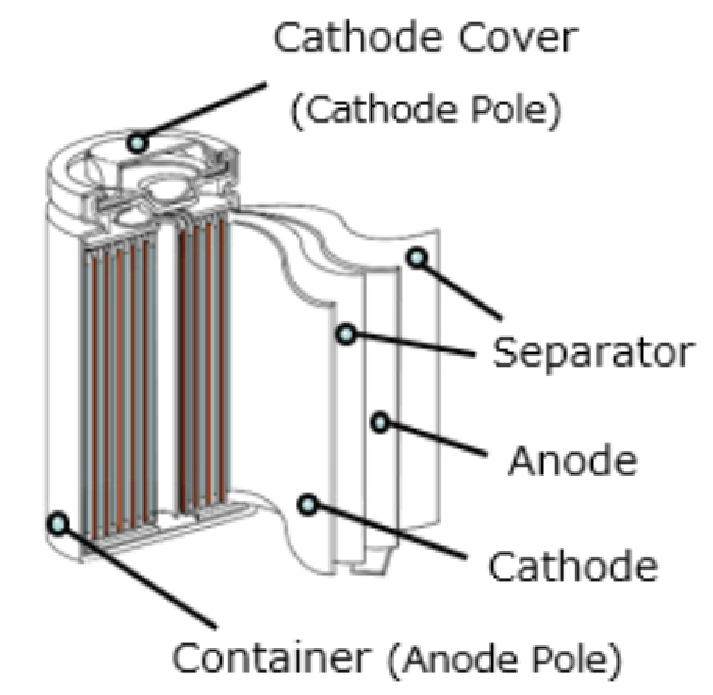
\includegraphics[width=0.4\linewidth]{Chapters/img/Cyrinder_battery.pdf}
		\centering
		\captionsetup{justification=centering,margin=2cm}
		\caption{โครงสร้างของเซลล์แบตเตอรี่ลิเธียมไอออนแบบทรงกระบอก}
		\label{fig:Li-ion Structure}
	\end{figure}
\end{center}
\begin{itemize}
 {\item 
 	อิเล็กโทรไลต์นั้นจะต้องสามารถส่งผ่านลิเธียมไอออนได้มากที่สุดเท่าที่สามารถส่งผ่านได้ภายใต้เงื่อนไขคือแบตเตอรี่นั้นจะต้องสามารถทำงานในสภาพแวดล้อมทั่วไปได้เช่นสามารถทำงานได้ในช่วงอุณหภูมิ -30$^\circ C$ 	 	     เพื่อที่ยานยนต์นั้นสามารถจอดได้ในกรณีที่จอดในช่วงเวลาที่อุณหภูมินั้นเย็นจัดจนถึงอุณหภูมิ +60$^\circ C$ ในกรณีที่อุณหภูมิของแบตเตอรี่นั้นสูงขึ้นเนื่องจากเป็นผลมาจากสภาพแวดล้อมภายนอกและเป็นผลมาจากการชาร์จ}
 {\item 
 	ในทำนองเดียวกันฉนวนที่กั้นระหว่างขั้วทั้งสองนั้นจะต้องสามารถส่งผ่านลิเธียมไอออนได้มากที่สุดเท่าที่จะสามารถทำได้ภายใต้เงื่อนไขเดียวกันกับอิเล็กโทรไลต์และจะต้องมีความสามารถทนความร้อนสูงแบบฉับพลัน
 }
 {\item 
 	ความเข้ากันได้ของวัสดุของขั้วของแบตเตอรี่นั้นจะต้องสามารถทำให้แบตเตอรี่มีความจุมากที่สุดเท่าที่จะสามารถเป็นไปได้โดยข้อสรุปของวัสดุต่างๆและปฏิกิริยาทางเคมีไฟฟ้านั้นเป็นไปดังรูปที่ 2 	       และแรงดันของเซลล์แบตเตอรี่นั้นขึ้นอยู่ความแตกต่างระหว่างคู่วัสดุที่ใช้นำมาทำเป็นขั้วของแบตเตอรี่ซึ่งแรงดันนั้นอาจจะถูกเปลี่ยนแปลงไปเนื่องจากการสูญเสียภายในเซลล์แบตเตอรี่อย่างเช่น การสูญเสีย IR losses เนื่องจากความสามารถในการส่งผ่านลิเธียมไอออนที่ไม่ดีในอิเล็กโทรไลท์ยกตัวอย่างเช่นถ้า LiFePO4 นั้นถูกใช้นำมาเป็นขั้วบวกและ Li4Ti5O12 เป็นขั้วลบของแบตเตอรี่จะทำให้ได้แรงดันเปิดวงจรปกตินั้นคือ$V_{oc}=V^+-V^-=1.95\ V$ โดย $V^+$ นั้นแทนศักย์ไฟฟ้าทางขั้วบวกของแบตเตอรี่ส่วน $V^-$ แทนศักย์ไฟฟ้าทางขั้วลบของแบตเตอรี่
 }
\end{itemize}

%===================================================================================================

\subsection{หลักการทำงานของแบตเตอรี่ลิเธียมไอออน}
\begin{center}
	\begin{figure}[!h]
		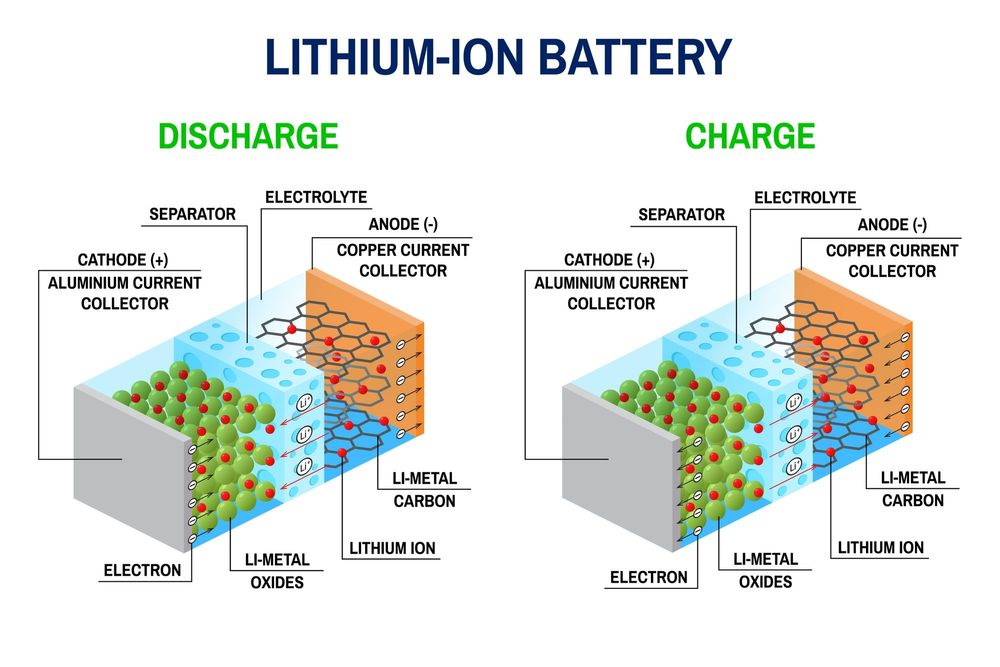
\includegraphics[width=0.6\linewidth]{Chapters/img/battery_structure.png}
			\centering
			\captionsetup{justification=centering,margin=2cm}
			\caption{ส่วนประกอบและการทำงานของเซลล์แบตเตอรี่ลิเธียมไอออน}
			\label{fig:Battery_Struc}
	\end{figure}
\end{center}

จากรูปที่\ref{fig:Battery_Struc} เป็นการทำงานของเซลล์แบตเตอรี่ลิเธียมไอออนในสภาวะการทำงานทั้งสองสภาวะดังนี้
\begin{itemize}
	{\item
		เมื่อเซลล์แบตเตอรี่อยู่ในสภาวะดิสชาร์จหรือทำงานเป็นแหล่งจ่ายพลังงาน อิเล็กตรอนจะเคลื่อนย้ายจากขั้วแอโนดผ่านตัวรับกระแสทั้งสองด้านและโหลดไปยังขั้วแคโทดในขณะเดียวกัน Li+ เคลื่อนย้ายจากขั้วแอโนดผ่านอิเล็กโทรไลต์และฉนวนไปยังขั้วแคโทด}
	{\item
		ในทางกลับกันเมื่อเซลล์แบตเตอรี่อยู่ในสภาวะการชาร์จ อิเล็กตรอนจะเคลื่อนย้ายจากขั้วแคโทดผ่านแหล่งจ่ายและตัวรับกระแสไปยังขั้วแอโนดในขณะเดียวกัน Li+ เคลื่อนย้ายจากขั้วแคโทดผ่านอิเล็กโทรไลต์และฉนวนไปยังขั้วแอโนด}
\end{itemize}
 ซึ่งเพื่อคงความเป็นกลางทางไฟฟ้าการเคลื่อนย้ายของอิเล็กตรอนและ Li+ นั้นจึงเกิดขึ้นพร้อมกันและเนื่องจากการเคลื่อนย้ายของอิเล็กตรอนก็มีผลทำให้เกิดกระแสไฟฟ้า
\newline ยกตัวอย่างเช่น พิจารณาแบตเตอรี่ลิเธียมแมงกานีสออกไซด์ (Lithium Manganese Oxide, LMO) เมื่อแบตเตอรี่อยู่ในสภาวะการชาร์จ Li+ เคลื่อนย้ายออกจาก LiMn2O4 ที่เป็นสารประกอบของขั้วแคโทดผ่านอิเล็กโทรไลต์และฉนวนไปสะสมอยู่ที่ชั้นคาร์บอนของกราไฟท์ที่เป็นขั้วแอโนดในทางตรงกันข้ามเมื่ออยู่ในสภาวะการดิสชาร์จ Li+ ที่สะสมอยู่ที่ชั้นคาร์บอนของกราไฟท์จากการชาร์จเคลื่อนย้ายผ่านอิเล็กโทรไลต์และฉนวนไปยัง LiMn2O4 ซึ่งปฏิกริยาที่เกิดขึ้นนี้เป็นดังนี้
 \newline ปฏิกิริยาทางขั้วแอโนด
\begin{equation}
LiMn_{2}O_{4} \Leftrightarrow Li_{1-x}Mn_{2}O_{4}+xLi^{+}+xe^{-} \label{eq:1}
\end{equation}
 \newline ปฏิกิริยาทางขั้วแคโทด
\begin{equation}
C+xLi^{+}+xe^{-} \Leftrightarrow Li_{x}C \label{eq:2}
\end{equation}
\newline ปฏิกิริยาทั้งระบบ
\begin{equation}
LiMn_{2}O_{4}+C \Leftrightarrow Li_{1-x}Mn_{2}O_{4}+Li_{x}C \label{eq:3}
\end{equation}
%===================================================================================================
\subsection{ลักษณะของแบตเตอรี่ลิเธียมไอออน}
เซลล์แบตเตอรี่ลิเธียมไอออนมีรูปลักษณ์ภายนอกที่นิยมในท้องตลาดอยู่ 3 ลักษณะดังนี้ ทรงกระบอก ทรงกล่อง และแบบแผ่น ซึ่งภายในจะมีลักษณะเป็นแบบพันรอบหรือแบบชั้นนั้นจะขึ้นอยู่กับลักษณะภายนอก
ตัวถังภายนอกของเซลล์แบตเตอรี่นั้นทำจากโลหะเช่น สแตนเลสหรืออลูมิเนียมสำหรับเซลล์แบบทรงกระบอกและทรงกล่อง อลูมิเนียมแผ่นสำหรับเซลล์แบบแผ่น ตัวถังของเซลล์แบตเตอรี่มีหน้าที่ที่สำคัญมากกว่าเป็นเพียงแค่ภาชนะบรรจุส่วนประกอบภายในซึ่งหน้าที่ที่สำคัญมากอย่างแรกนั่นคือป้องกันส่วนประกอบภายในจากความชื้นและแก็สออกซิเจนจากภายนอกซึ่งกัดกร่อนหรือทำให้ขั้วของเซลล์นั้นเป็นสนิม
และทำหน้าที่เป็นฉนวนระหว่างขั้วบวกและขั้วลบระหว่างเซลล์แบตเตอรี่หน้าที่ที่สำคัญอีกอย่างหนึ่งของตัวถังนั่นคือลดความดันจากภายในของเซลล์แบตเตอรี่ในขณะที่เซลล์ทำงานผิดปกติจนอาจทำให้ผิดรูปร่างทั้งนี้เพื่อให้ยังคงพื้นที่สำหรับเซลล์แบตเตอรี่
ในโมดูลแบตเตอรี่แต่สำหรับตัวถังแบบแผ่นนั้นไม่สามารถทำได้
\newline\hspace*{2cm} ดังตารางที่\ref{tab:compare_shape} เป็นการสรุปโดยสังเขปของเซลล์แบตเตอรี่ทั้ง 3 ลักษณะทั้งนี้เซลล์แบตเตอรี่แต่ละแบบนั้นมีข้อดีและข้อเสียแตกต่างกันแล้วแต่การนำไปประยุกต์ใช้
%Table 1
%\begin{center}
%	\begin{figure}[!h]
%		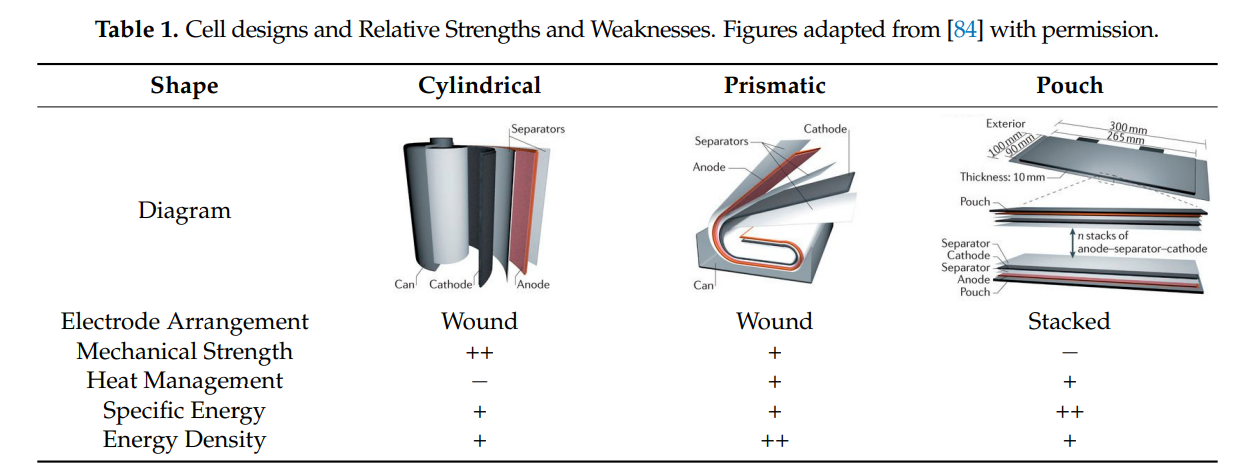
\includegraphics[width=0.6\linewidth]{Chapters/img/Compare_Cell.png}
%			\centering
%			\captionsetup{justification=centering,margin=2cm}
%			\caption{เป็นการสรุปโดยสังเขปของเซลล์แบตเตอรี่ทั้ง 3 ลักษณะทั้งนี้เซลล์แบตเตอรี่แต่ละแบบนั้นมีข้อดีและข้อเสียแตกต่างกันแล้วแต่การนำไปประยุกต์ใช้}
%	\end{figure}
%\end{center}
\begin{table}[H]
\caption{ตารางเปรียบเทียบรูปร่างเซลล์แบตเตอรี่อย่างง่าย}
\centering
\begin{tblr}{
  cells={valign=m,halign=c},
  row{1}={font=\bfseries,rowsep=8pt},
  column{1} = {5cm}
}
%\begin{tabular}{ | c c c c | }
%	\hline \\
      รูปร่าง & แบบทรงกระบอก & แบบทรงสี่เหลี่ยม & แบบซอง \\ \hline
 	&
 	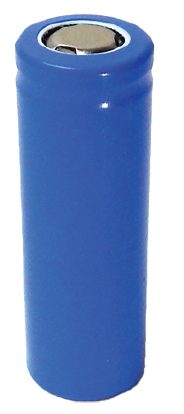
\includegraphics[scale=0.5,valign=c]{Chapters/img/Cyrinder_battery_table.png}
 	&
 	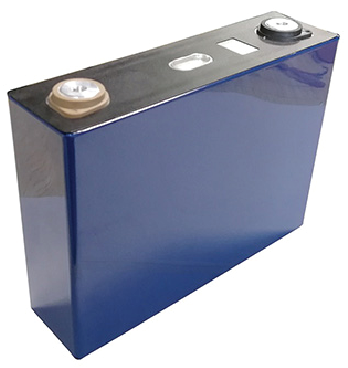
\includegraphics[scale=0.5,valign=c]{Chapters/img/Prismatic_battery.png}
 	&
	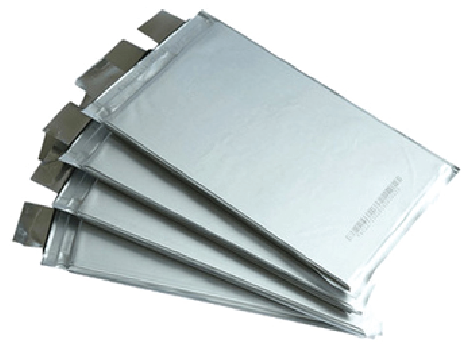
\includegraphics[scale=0.5,valign=c]{Chapters/img/Pounch_battery.png} \\
	การจัดวางขั้วของแบตเตอรี่ & พันรอบ & พันรอบ & วางซ้อน\\
	ความแข็งแรงทางกล & ++ & + & -\\
	การระบายความร้อน & - & + & +\\
	พลังงานจำเพาะ & + & + & ++\\
	ความหนาแน่นพลังงาน & + & ++ & + \\ \hline
%\end{tabular}
\end{tblr}
\label{tab:compare_shape}
\end{table}
%================================================================================================
\subsection{คุณลักษณะของแบตเตอรี่ลิเธียมไอออน}
ในหัวข้อนี้จะสรุปคำศัพท์หรือคุณลักษณะต่างๆที่ใช้ในการระบุ เปรียบเทียบ และจำแนกแบตเตอรี่ลิเธียมไอออนซึ่งเป็นพื้นฐานสำคัญดังนี้
\begin{itemize}
	{\item
		C rate และ E rate กระแสดิสชาร์จบ่อยครั้งจะแสดงอยู่ใน C-rate ซึ่ง C-rate คืออัตราการดิส-ชาร์จต่อความจุสูงสุดของแบตเตอรี่เช่น 1C      	  หมายถึงกระแสดิสชาร์จนี้จะดิสชาร์จแบตเตอรี่หมดภายใน 1 ชั่วโมงสำหรับแบตเตอรี่ 100Ah กระแสดิสชาร์จจะเท่ากับ 100A ที่ 5C นั้นกระแสดิสชาร์จจะอยู่ที่ 500A และที่ C/2 
		กระแสดิสชาร์จจะอยู่ที่ 50A ในทำนองเดียวกัน E-rate คืออัตราพลังงานไฟฟ้าดิสชาร์จ 1E หมายถึงพลังงานไฟฟ้าที่ใช้ในการดิสชาร์จหมดภายใน 1 ชั่วโมง}
	{\item
		State of Charge (SOC) หมายถึงการแสดงสถานะความจุของแบตเตอรี่เทียบกับความจุสูงสุดของแบตเตอรี่เป็นเปอร์เซ็นต์}
	{\item
		Depth of Discharge (DOD) หมายถึงเปอร์เซ็นต์ความจุของแบตเตอรี่ที่ถูกดิสชาร์จไปเทียบกับความจุสูงสุดของแบตเตอรี่}
	{\item
		แรงดันที่ขั้ว (Terminal Voltage) หมายถึงแรงดันระหว่างขั้วของแบตเตอรี่ในขณะต่อโหลดซึ่งแรงดันนั้นขึ้นอยู่กับ SOC และกระแสชาร์จหรือดิสชาร์จ}
	{\item
		แรงดันเปิดวงจร (Open-circuit Voltage, OCV) หมายถึงแรงดันระหว่างขั้วของแบตเตอรี่ในขณะที่ไม่มีโหลดซึ่งขึ้นอยู่กับ SOC เช่นกัน}
	{\item
		แรงดันปกติ (Nominal Voltage) หมายถึงการรายงานแรงดันของแบตเตอรี่หรือแรงดันอ้างอิงของแบตเตอรี่}
	{\item
		แรงดันตัด (Cut-off Voltage) หมายถึงแรงดันต่ำที่สุดที่แบตเตอรี่สามารถจ่ายได้หรือหมายถึงแรงดันที่แสดงถึงสถานะของแบตเตอรี่ที่หมดแล้ว}
	{\item
		ความจุหรือความจุปกติ (Capacity or Nominal Capacity, Ah) หมายถึงความจุคูลอมบิกเมตริกหรือก็คือแอมแปร์ชั่วโมงทั้งหมดที่แบตเตอรี่สามารถดิสชาร์จได้จาก 100\%SOC จนถึงแรงดันตัด}
	{\item
		พลังงานหรือพลังงานปกติ (Energy or Nominal Energy, Wh) หมายถึงความจุพลังงานของแบตเตอรี่หรือก็คือวัตต์ทั้งหมดที่แบตเตอรี่สามารถดิสชาร์จได้จาก 100\%SOC จนถึงแรงดันตัด}
	{\item
		ไลฟ์ไซเคิล (Cycle Life) หมายถึงจำนวนรอบในการดิสชาร์จของแบตเตอรี่ที่สามารถดิสชาร์จได้ก่อนที่จะเสื่อมสภาพตามเกณฑ์อย่างไรก็ตามสภาพการทำงานของแบตเตอรี่นั้นมีปัจจัยหลายอย่างนอกจากจำนวนรอบการดิสชาร์จเช่น ความชื้นและอุณหภูมิ}
	{\item
		พลังงานจำเพาะ (Specific Energy, Wh/kg) หมายถึงพลังงานปกติต่อมวลของแบตเตอรี่บางครั้งอาจจะหมายถึงความหนาแน่นพลังงานโดยน้ำหนักของแบตเตอรี่}
	{\item
		กำลังไฟฟ้าจำเพาะ (Specific Power, W/kg) หมายถึงกำลังไฟฟ้าสูงสุดต่อมวลของแบตเตอรี่}
	{\item
		ความหนาแน่นพลังงาน (Energy Density, Wh/L) หมายถึงพลังงานปกติต่อหนึ่งหน่วยปริมาตรบางครั้งอาจจะหมายถึงความหนาแน่นพลังงานโดยปริมาตร}
	{\item
		ความหนาแน่นกำลังไฟฟ้า (Power Density, W/L) หมายถึงกำลังไฟฟ้าสูงสุดต่อหนึ่งหน่วยปริมาตรของแบตเตอรี่}
	{\item
		กระแสดิสชาร์จต่อเนื่องสูงสุด (Maximum Continuous Discharge Current) หมายถึงกระ-แสดิสชาร์จสูงสุดที่แบตเตอรี่สามารถดิสชาร์จได้อย่างต่อเนื่องข้อจำกัดนี้จะถูกกำหนดโดยโรงงานแบตเตอรี่เพื่อป้องกันอัตราการดิสชาร์จที่มากเกินไปซึ่งอาจจะทำให้แบตเตอรี่เสียหายหรือลดความจุลงได้}
	{\item
		กระแสพัลส์สูงสุดใน 30 วินาที (Maximum 30-sec Discharge Pulse Current) หมายถึงกระแสดิสชาร์จสูงสุดฉับพลันโดยดิสชาร์จเป็นเวลา 30 วินาที}
	{\item
		แรงดันชาร์จ (Charge Voltage) หมายถึงแรงดันของแบตเตอรี่เมื่อแบตเตอรี่ชาร์จเต็มแล้ว}
	{\item
		แรงดันลอยตัว (Float Voltage) หมายถึงแรงดันคงที่ที่แบตเตอรี่ชาร์จจนเต็มแล้วก่อนที่จะเกิดการดิสชาร์จเองภายใน}
\end{itemize}
%====================================================================================================
\subsection{แบตเตอรี่ลิเธียมไอออนชนิดต่างๆ}
	ในหัวข้อนี้จะกล่าวถึง สรุปข้อแตกต่าง ของแบตเตอรี่ลิเธียมไอออนแต่ละชนิดแบตเตอรี่ลิเธียมไอออนในปัจจุบันนั้นเป็นที่นิยมกันอยู่ในตลาดทั้งสิ้น 6 ชนิดซึ่งแต่ละชนิดนั้นโดยทั่วไปแล้วจะจำแนกตวามวัสดุที่นำมาใช้เป็นขั้วบวกของแบตเตอรี่ยกเว้นแบตเตอรี่ลิเธียมไอออนชนิดิเธียมไท-ทาเนต(Lithium Titanate, LTO) ที่ใช้วัสดุที่ใช้นำมาเป็นขั้วลบคือ Li4Ti5O12 มาทำการจำแนก ซึ่งแบตเตอรี่ลิเธียมไอออนทั้ง 6 ชนิดที่ได้อ้างถึงมีด้วยกันดังนี้ 
\subsubsection*{แบตเตอรี่ลิเธียมโคบอลต์ออกไซด์\\ (Lithium Cobalt Oxide Battery)}
	แบตเตอรี่ลิเธียมโคบอลต์ออกไซด์ถูกพัฒนาขึ้นครั้งแรกโดยบริษัท Sony ในปี 1991 แบตเตอรี่ลิเธียมโคบอลต์ออกไซด์ถูกใช้กับอุปกรณ์อิเล็กทรอนิกส์ส่วนตัวเป็นส่วนใหญ่เช่น แล็ปท็อป กล้องถ่ายรูป ฯลฯ เป็นต้นเนื่องจากมีความหนาแน่นของพลังงานสูง อายุการใช้งานนาน และผลิตง่าย แต่แบตเตอรี่ลิเธียมโคบอลต์ออกไซด์นั้นมีปฏิกิริยาสูงดังนั้นจึงทำให้ไม่เสถียรทางความร้อนและต้องการการวัด ตรวจจับ แสดงผลตลอดช่วงเวลาทำงานเพื่อความปลอดภัยและเนื่องจากโคบอลต์นั้นเป็นวัสดุที่หาได้ยากทำให้แบตเตอรี่ลิเธียมโคบอลต์ออกไซด์มีราคาแพงและด้วยปัญหาด้านความร้อนแบตเตอรี่ลิเธียมโคบอลต์ออกไซด์จึงไม่ค่อยเหมาะกับการนำไป
ใช้ในยานยนต์ไฟฟ้า
\newline\hspace*{2cm}
อย่างไรก็ตามแบตเตอรี่ลิเธียมโคบอลต์ออกไซด์นั้นได้ถูกนำไปใช้กับยานยนต์ไฟฟ้าอย่าง Tesla Roadster และ Smart Fortwo Electric drive(ED)
\subsubsection*{แบตเตอรี่ลิเธียมแมงกานีสออกไซด์\\ (Lithium Manganese Oxide Battery, LMO)}
	แบตเตอรี่ลิเธียมแมงกานีสออกไซด์ได้ถูกนำเสนอขึ้นเป็นครั้งแรกในช่วงต้นทศวรรษ 1980 และใช้เวลากว่า 15 ปีกว่าจะนำมาจำหน่ายในท้องตลาด ด้วยสถาปัตยกรรมโครงสร้างทางด้านเคมีช่วยเพิ่มการเคลื่อนย้ายของไอออน(Li+)ในอิเล็กโทรดเป็นผลทำให้ลดความต้านทานภายในของแบตเตอรี่และช่วยให้ทนกระแสไฟฟ้าได้มากขึ้นนั่นหมายความว่าสามารถเพิ่มความเร็วในการชาร์จหรือเพิ่มกระแสไฟฟ้าในการชาร์จและสามารถใช้กระแสดิสชาร์จที่สูงได้ ซึ่งข้อดีทางเคมีนี้ทำให้แบตเตอรี่ลิเธี-ยมแมงกานีสออกไซด์นั้นมีเสถียรภาพทาทงด้านความร้อนมากกว่าแบตเตอรี่ลิเธียมโคบอลต์ออกไซด์แต่มีข้อเสียนั่นคือมีความจุน้อยและอายุการใช้งานสั้นกว่าโดยประมาณ 33\% 
\newline\hspace*{2cm}ส่วนมากแบตเตอรี่ลิเธียมแมงกานีสออกไซด์นั้นถูกผสมเข้ากับแบตเตอรี่ลิเธียมแมงกานีสโคบอลต์ออกไซด์เพื่อเพิ่มพลังงานจำเพาะและอายุการใช้งานซึ่งแบตเตอรี่โดยการผสมนี้ในอดีตเคยถูกใช้ในยานยนต์ไฟฟ้าหลายรุ่นเช่น Nissan Leaf, Chevy volt, BMW i3
\subsubsection*{แบตเตอรี่ลิเธียมฟอสเฟต\\ (Lithium Iron Phosphate, LFP)}
	ในปี 1996 กลุ่มนักวิจัยในมหาวิทยาลัยเทกซัสออสติน(The University of Texas at Austin) ค้นพบว่าฟอสเฟตนั้นสามารถนำมาใช้เป็นอิเล็กโทรดของแบตเตอรี่ลิเธียมไอออนได้ ฟอสเฟตนั้นช่วยให้มีความสเถียรต่อการชาร์จเกิน(Over charge)และช่วยเพิ่มความทนทานต่อความร้อน แบตเตอรี่ลิเธียมฟอสเฟตมีความสามารถทางเคมีไฟฟ้าที่ดีเช่น มีความต้านทานต่ำ เป็นต้น มีช่วงอุณหภูมิการทำงานที่กว้างคือ +60$^{\circ}C$ ถึง -30$^{\circ}C$ และเกิดปฏิกิริยาคายความร้อนสูง(Thermal runaway)ได้ยากแต่มีการดิสชาร์จเองสูงมากกว่าแบตเตอรี่ลิเธียมไอออนชนิดอื่นๆทำให้มีปัญหาทางด้านสมดุลของอายุแบตเตอรี่ซึ่งสามารถใช้อุปกรณ์อิเล็กทรอนิกส์มาช่วยควบคุมปัญหานี้ได้เช่น BMS แต่ก็ทำให้ราคาของแบตเตอรี่นั้นสูงขึ้น
\newline\hspace*{2cm}
ด้วยประสิทธิภาพอัตราส่วนกำลังไฟฟ้าต่อน้ำหนักและความปลอดภัยสูงนั่นทำให้แบตเตอรี่ลิเธียมฟอสเฟตนิยมใช้มากในรถบ้าน มีการร่วมมือกันระหว่างบริษัทในประเทศเยอรมันได้แก่ ElektroFahrzeuge Stuttgart และ WOF ได้ทำรถบ้านที่ใช้ระบบไฟฟ้าทั้งหมดเจ้าแรกส่งออกสู่ตลาดซึ่งในระบบไฟฟ้านี้ก็นำแบตเตอรี่ลิเธียมมาใช้ด้วยเช่นกัน
\subsubsection*{เเบตเตอรี่ลิเธียมนิกเกิลแมงกานีสโคบอลต์ออกไซด์\\ (Lithium Nickel Manganese Cobalt Oxide Battery, NMC)}
	แบตเตอรี่นิกเกิลแมงกานีสโคบอลต์ออกไซด์สามรถออกแบบให้มีพลังงานจำเพาะสูงหรือกำลังไฟฟ้าได้ซึ่งเป็นผลดีมาจากการผสมกันระหว่างโลหะ 2 ชนิดคือนิกเกิลและแมงกานีส นิกเกิลนั้นทำให้พลังงานจำเพาะสูงแต่มีความเสถียรต่ำส่วนแมงกานีสนั้นทำให้ความต้านทานภายในต่ำแต่มี
	\\ข้อเสียคือทำให้พลังงานจำเพาะต่ำซึ่งอัตราส่วนของผสมโลหะต่างๆของแบตเตอรี่ลิเธียมนิกเกิลแมงกานีสโคบอลต์ออกไซด์นั้นขึ้นอยู่กับแต่ละโรงงานผลิตซึ่งมีดังนี้ NMC111(ความจุ 154 $Ah\cdot kg^{-1}$ ที่ 0.1C) NMC442 NMC622 และในปัจจุบัน NMC811(ความจุ > 185 $Ah\cdot kg^{-1}$ ที่ 0.1C)	
\newline\hspace*{2cm}การผสมกันระหว่างแมงกานีสและนิกเกิลช่วยเสริมข้อดีของกันและกันทำให้แบตเตอรี่ลิเธียมนิเกิลแมงกานีสโคบอลต์ออกไซด์เป็นแบตเตอรี่ลิเธียมไอออนที่ประสบความสำเร็จมากที่สุดและเหมาะสำหรับการนำไป
	ใช้กับยานยนต์ไฟฟ้าซึ่งปัจจุบันแบตเตอรี่ชนิดนี้เป็นที่ต้องการอย่างมากเนื่องจากพลังงานจำเพาะสูงและคุณลักษณะทางความร้อนที่ดีจากที่กล่าวมาแบตเตอรี่ลิเธียมนิกเกิลแมงกานีสโคบอลต์ออกไซด์
	ถูกนำไปใช้กับยานยนต์ไฟฟ้าหลายรุ่นด้วยกันเช่น Nissan Leaf, Chevy Volt, BMW i3
\subsubsection*{แบตเตอรี่นิกเกิลโคบอลต์อลูมินัมออกไซด์์\\ (Nickel Cobalt Aluminum Oxide Battery, NCA)}
แบตเตอรี่นิกเกิลโคบอลต์อลูมินัมออกไซด์เกิดขึ้นช่วงปี 1999 แบตเตอรี่ลิเธียมโคบอล-ต์อลูมินัมออกไซด์ มีความคล้ายคลึงกับแบตเตอรี่นิกเกิลแมงกานีสโคบอลต์ออกไซด์โดยให้พลังงานจำเพาะและกำลังไฟฟ้าจำเพาะที่สูงและมีอายุการใช้งานที่ยาวนานแต่ไม่ค่อยมี
ความปลอดภัยเท่ากับแบตเตอรี่ลิเธียมไอออนชนิดอื่นๆ สำหรับการประยุกต์ใช้ในยานยนต์ไฟฟ้านั้นต้องการการตรวจจับและแสดงผลอยู่ตลอดเพื่อความปลอดภัย มีต้นทุนการผลิตสูงและไม่เหมาะกับการไปใช้กับงานประเภทอื่นๆ
\newline\hspace*{2cm} 
อย่างไรก็ตาม Tesla เป็นบริษัทเดียวที่ใช้แบตเตอรี่ชนิดนี้และอ้างว่าแบตเตอรี่นิกเกิล\\โคบอลต์อลูมินัมออกไซด์ของ Tesla นั้นใช้โคบอลต์ในการผลิตน้อยกว่า NMC811 ซึ่งใช้โคบอลต์เพียง 15\% ซึ่งแบตเตอรี่นิกเกิลโคบอลต์อลูมินัมออกไซด์ถูกนำไปใช้ใน Tesla Model 3 และ Model S ช่วงแรกๆในปี 2012
\subsubsection*{แบตเตอรี่ลิเธียมไททาเนต\\ (Lithium Titanate, LTO)}
	การใช้ลิเธียมไททาเนตในแบตเตอรี่นั้นเกิดขึ้นในปี 1980 ลิเธียมไททาเนตถูกแทนที่กรา-ไฟท์ในการนำมาใช้เป็นอิเล็กโทรดของแบตเตอรี่ลิเธียมไอออนและทำให้อยู่ในโครงสร้างเฉพาะทางเคมีโดยอิเล็กโทรดขั้วตรงข้ามอาจจะใช้ลิเธียมแมงกานีสออกไซด์ก็ได้ ลิเธียมไททาเนตที่ถูกทำให้อยู่ในโครงสร้างเฉพาะทางเคมีนี้ได้รับการยอมรับว่าเป็นวัสดุที่มีประโยชน์มากเนื่องจากระหว่างการเกิดปฏิกิริยาลิเธียชั่น(Lithiation)หรือการส่งผ่านไอออน Li+ ลิเธียมไททาเนตนั้นจะไม่มีการเปลี่ยนแปลงปริมาตรเป็นผลทำให้มีอายุการใช้งานที่นานขึ้นมากคู่กับความปลอดภัยจากการดิสชาร์จและชาร์จที่\\สเถียรมากราวๆ 1.55V vs Li/Li+ ลิเธียมไททาเนตนั้นนำไฟฟ้าได้ไม่ค่อยดีและค่าสัมประสิทธิ์การแพร่ของไอออน Li+ น้อยทำให้ไม่เหมาะกับการใช้งานที่กำลังไฟฟ้าสูงแต่อย่างไรก็ตามปัญหานี้สามารถช่วยได้โดยลดระยะทางการเคลื่อนย้ายของไอออน Li+ ในโครงสร้างของแบตเตอรี่เพื่อส่งผ่านไอออนได้ดีขึ้นเพิ่มการนำไฟฟ้าได้โดยการโดป(Doping) เคลือบผิว(Surface Coating) ผสม(Forming)กับวัสดุที่นำไฟฟ้าได้ดีอย่างคาร์บอน
\newline\hspace*{2cm}
แบตเตอรี่ลิเธียมไททาเนตถูกใช้กับยานยนต์ไฟฟ้าเฉพาะในประเทศญี่ปุ่นอย่าง Mitsubishi i-MiEV, Honda และระบบรถบัสไฟฟ้าสาธารณะ(Tosa) และเนื่องจากมีความปลอดภัยสูงแบตเตอรี่ลิเธียมไททาเนตจึงถูกนำไปใช้ในอุปกรณ์การแพทย์ด้วย
\begin{center}
	\begin{figure}[H]
		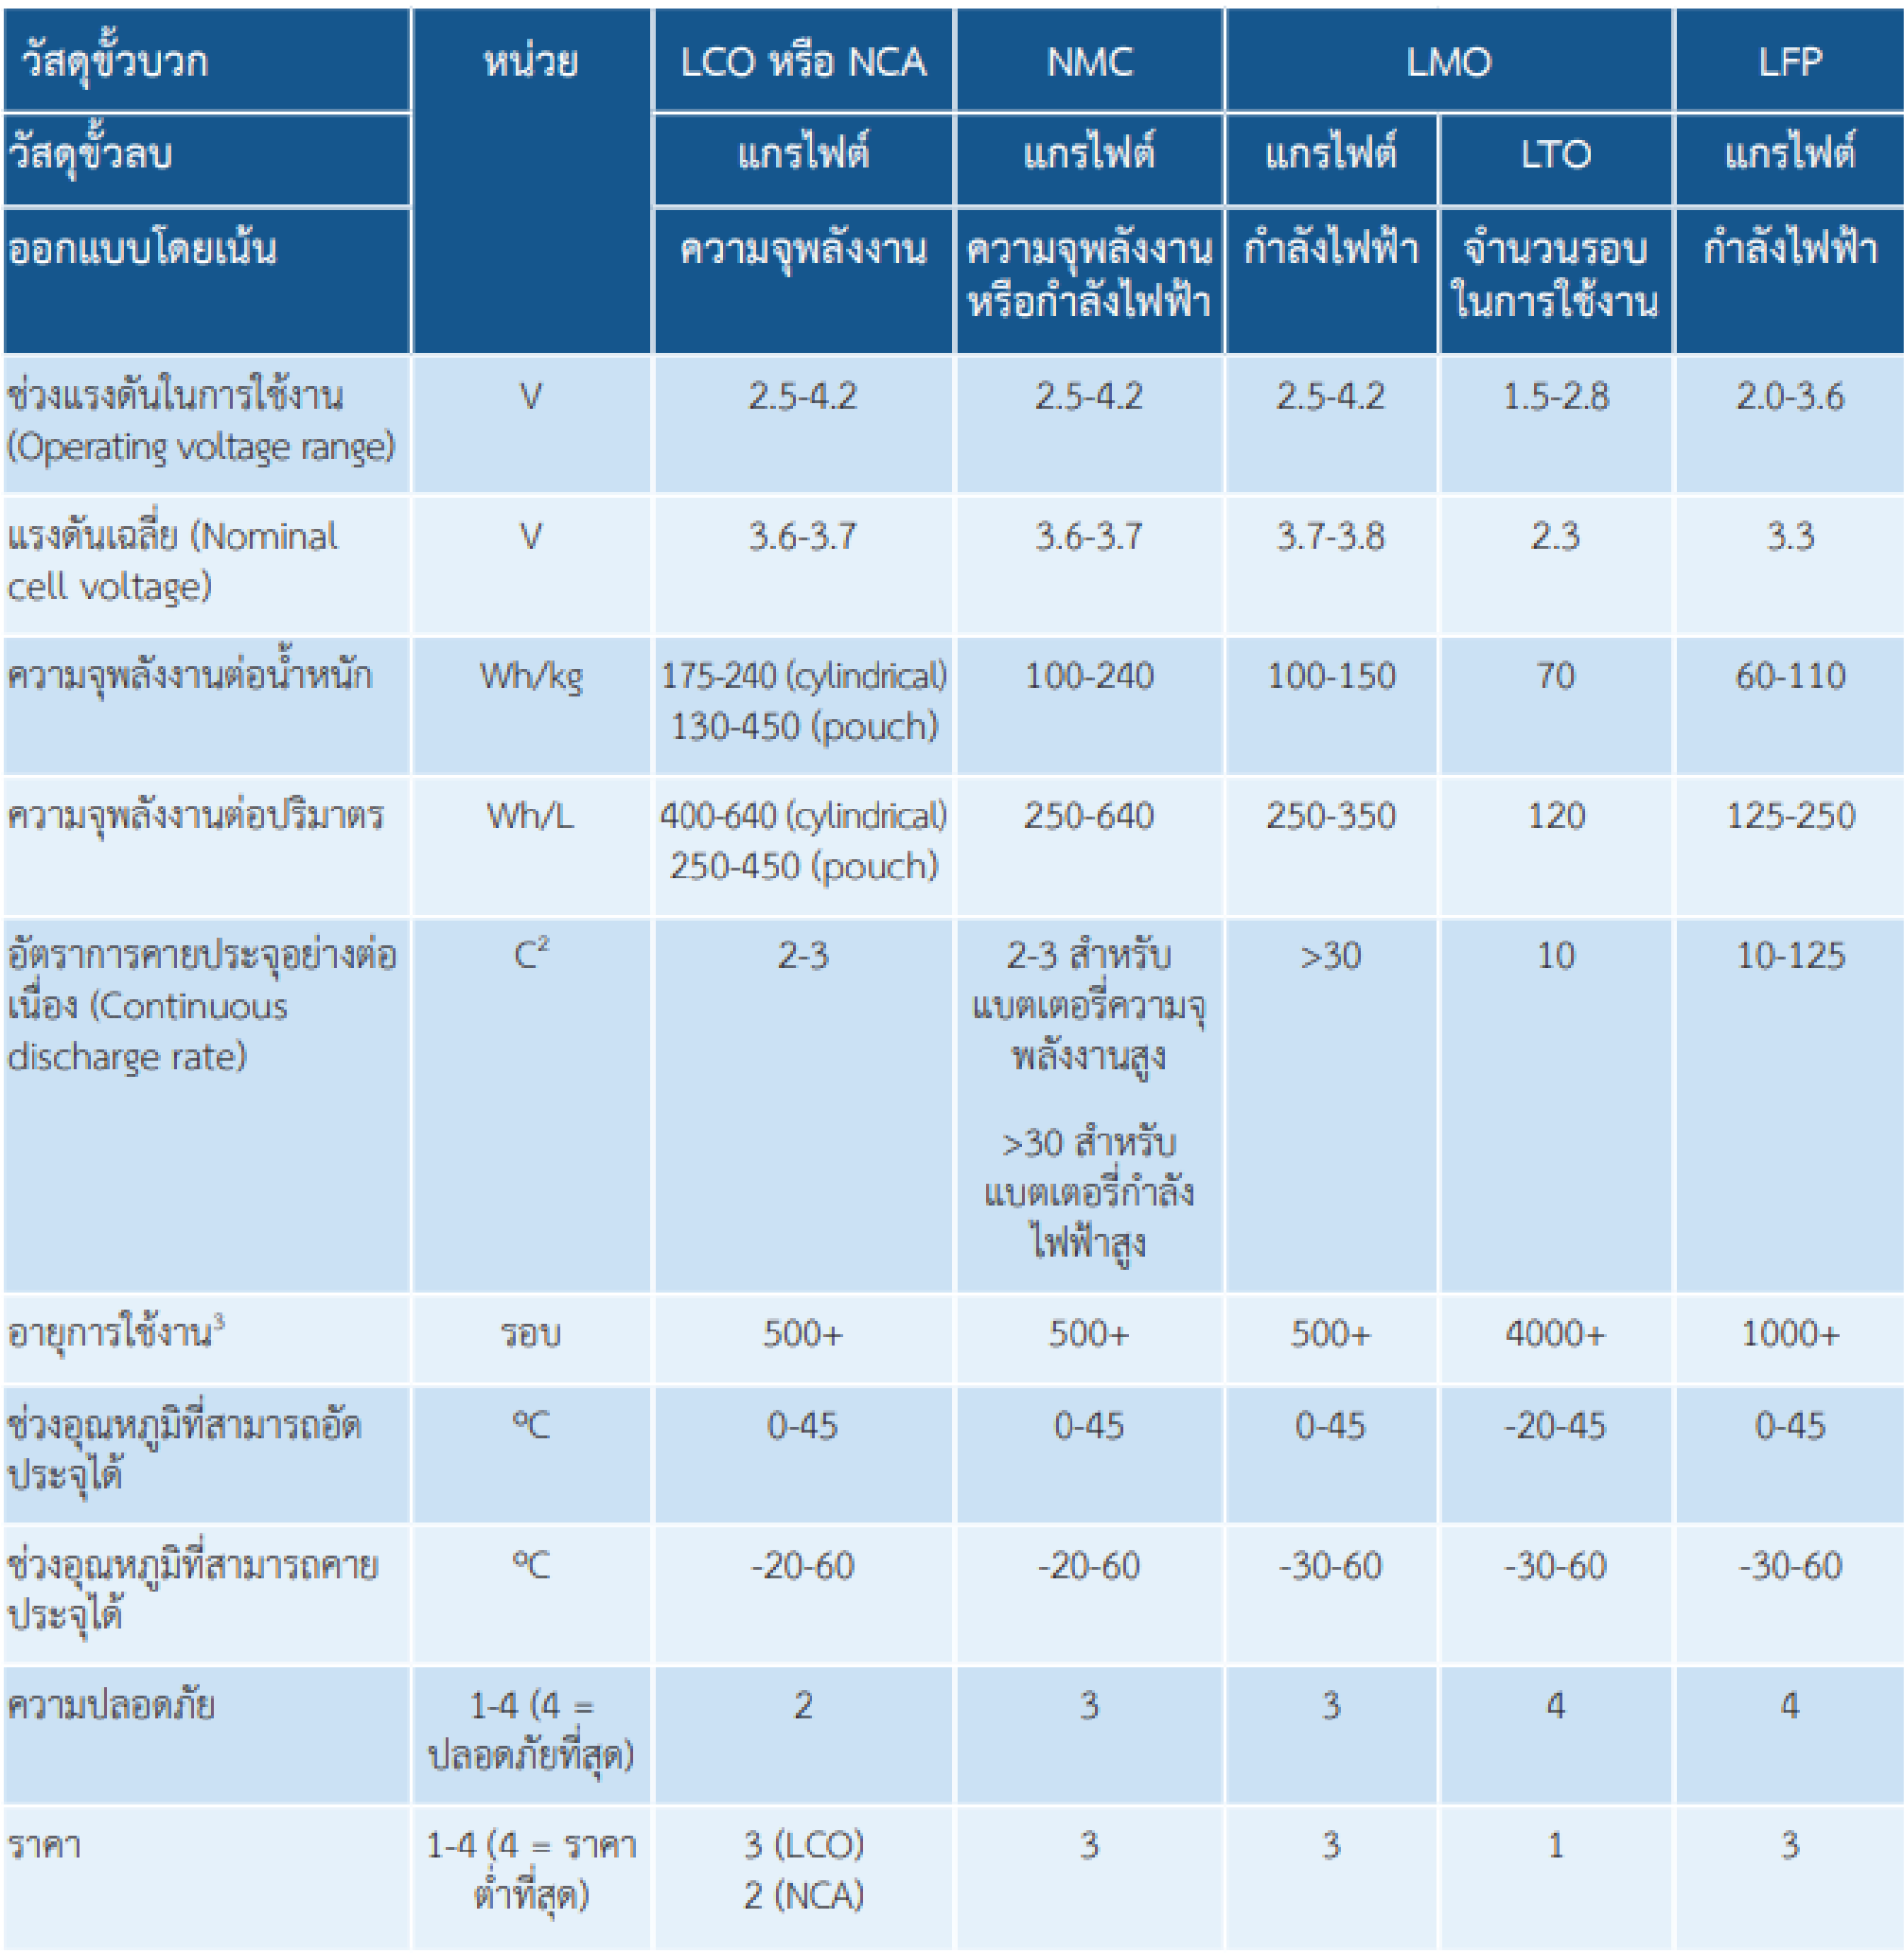
\includegraphics[width=1\linewidth]{Chapters/img/Compare_Spec_Batteries.png}
			\centering
			\captionsetup{justification=centering,margin=2cm}
			\caption{เปรียบเทียบคุณสมบัติต่างๆของแบตเตอรี่ลิเธียมไอออน}
	\end{figure}
\end{center}
%========================================================================================
\begin{center}
	\begin{figure}[H]
		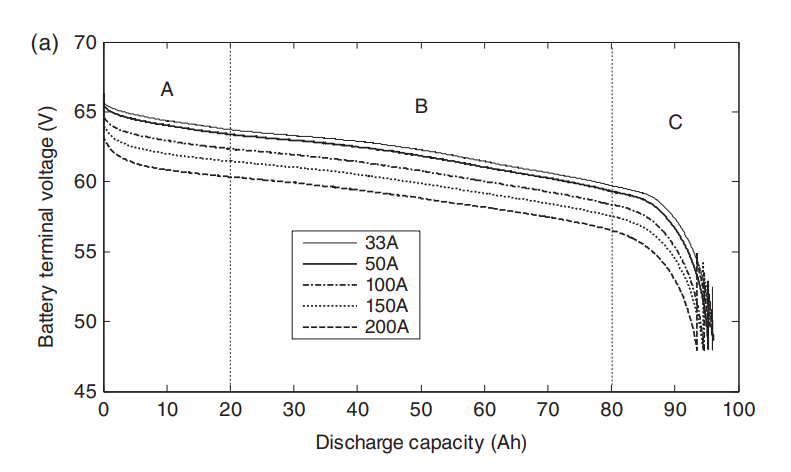
\includegraphics[width=0.6\linewidth]{Chapters/img/IV_a.png}
			\centering
			\captionsetup{justification=centering,margin=2cm}
			\caption{กราฟการทดสอบการดิสชาร์จ(ก)}
	\end{figure}
\end{center}
\section{ประสิทธิภาพอัตราการดิสชาร์จของแบตเตอรี่ลิเธียมไอออน}
ในหัวข้อนี้และหัวข้อถัดไป 2.3 จะใช้โมดูลแบตเตอรี่ความจุ 100Ah ที่ประกอบไปด้วยเซลล์แบตเตอรี่ลิเธียมแมงกานีสออกไซด์ 16 เซลล์ในการทดสอบซึ่งความสัมพันธ์ระหว่างแรงดันกับความจุของโมดูลแบตเตอรี่ภายใต้กระแสดิสชาร์จที่ต่างกัน ณ อุณหภูมิห้องดังรูปที่ 3 ส่วนรูปที่ 4 คือรูปขยายบางส่วนของรูปที่ 3 ที่จุด M1, M2, M3, M4 และ M5 โมดูลแบตเตอรี่มีความจุที่ 93.43Ah, 94.43Ah, 94.55Ah, 95.24Ah และ 95.96 Ah ตามลำดับซึ่งดิสชาร์จด้วยกระแสไฟฟ้าขนาด 200A(2C), 150A(1.5C), 100A(1C), 50A(0.5C) และ 33A(1/3C) ตามลำดับและแรงดันเปิดวงจรหลังจากที่ทำพักโมดูลแบตเตอรี่ทิ้งไว้เป็นเวลา 1 ชั่วโมงคือ 54.85V, 54.15V, 53.44V, 52.83V และ 52.48V ตามลำดับ
\begin{center}
	\begin{figure}[H]
		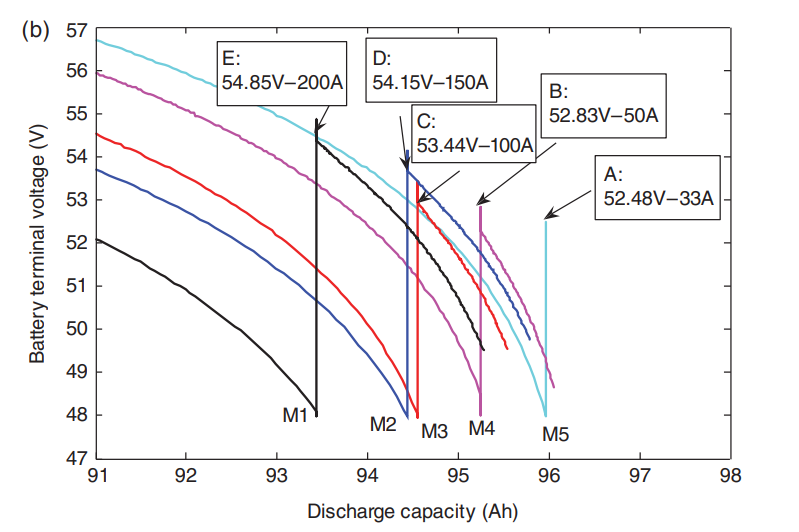
\includegraphics[width=0.6\linewidth]{Chapters/img/IV_b.png}
			\centering
			\captionsetup{justification=centering,margin=2cm}
			\caption{กราฟการทดสอบการดิสชาร์จ(ข)}
	\end{figure}
\end{center}
ซึ่งจะเห็นได้ว่าแรงดันเปิดวงจรของโมดูลแบตเตอรี่เพิ่มขึ้นเมื่อกระแสดิสชาร์จเพิ่มขึ้นและการดิสชาร์จด้วยกระแส 200A ทำให้ความจุของโมดูลแบตเตอรี่นั้นลดลงเพียง 2.6\% เมื่อเทียบกับการดิสชาร์จด้วยกระแส 33A โดยการทดลองนี้แสดงให้เห็นถึงความสามารถในอัตราการดิสชาร์จที่ดีของโมดูลแบตเตอรี่ลิเธียมแมงกานีสออกไซด์เนื่องจากสามารถดิสชาร์จที่กระแสขนาดใหญ่ได้ในขณะที่ความจุเเละแรงดันเพิ่มขึ้นแต่ในทางตรงกันข้ามอุณภูมิของโมดูลแบตเตอรี่
เพิ่มขึ้นอย่างรวดเร็วเมื่อดิสชาร์จด้วยกระแสขนาดใหญ่จากรูปที่ 3 จะเห็นได้ว่าแรงดันของโมดูลแบตเตอรี่จะคงที่มากที่สุดเมื่อ SOC อยู่ที่ช่วง 20\%-80\%(บริเวณ B) เนื่องจากปฏิกริยาไฟฟ้าเคมีในเซลล์แบตเตอรี่นั้นทำงานได้อย่างมีประสิทธิภาพมากที่สุดและเนื่องจากความต้านทานภายในและความต้านทานที่ขั้วของเซลล์แบตเตอรี่เพิ่มขึ้นทำให้ประสิทธิภาพการดิสชาร์จนั้นลดลงมากในช่วง SOC 0\% - 20\%
(บริเวณ A) และช่วง 80\% - 100\%(บริเวณ C) และแรงดันของโมดูลแบตเตอรี่ลดลงอย่างมากเมื่อทำการดิสชาร์จจนหมดดังนั้นการ\\ดิสชาร์จแบตเตอรี่จนหมดหรือใกล้หมดนั้นทำให้ประสิทธิภาพการดิสชาร์จลดลงและส่งผลเสียต่ออายุการใช้งานของแบตเตอรี่ด้วยและเพื่อประสิทธิภาพในการใช้งานสูงสุดและเพื่อเพิ่ม
อายุการใช้งานของแบตเตอรี่จึงควรจะใช้งานแบตเตอรี่ช่วงที่มีประสิทธิภาพการดิสชาร์จมากที่สุด
\begin{center}
	\begin{figure}[H]
		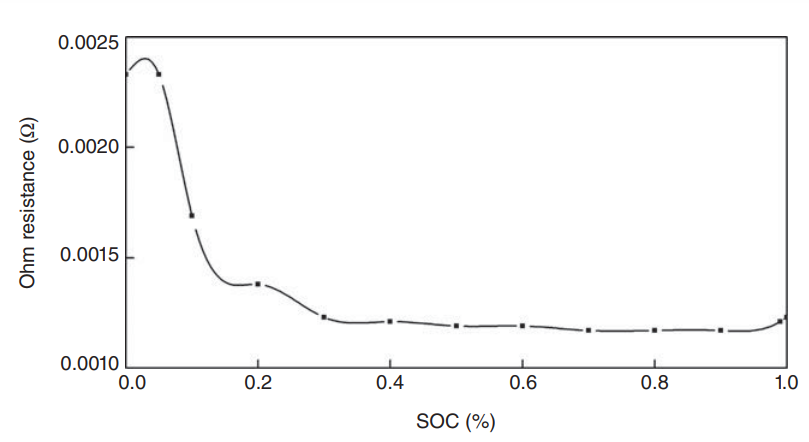
\includegraphics[width=0.6\linewidth]{Chapters/img/Resistance_vs_SOC.png}
			\centering
			\captionsetup{justification=centering,margin=2cm}
			\caption{กราฟแสดงความสัมพันธ์ระหว่างความต้านทานกับSOC}
	\end{figure}
\end{center}
%=============================================================================================
\subsection{ผลกระทบของอุณหภูมิต่อความจุของแบตเตอรี่}
โมลดูลแบตเตอรี่ลิเธียมแมงกานีสออกไซด์ถูกใช้ทดสอบที่กระแสดิสชาร์จคงที่ 1/3C ณ อุณหภูมิตั้งแต่ -30$^{\circ}C$ ถึง 50$^{\circ}C$ โดยเพิ่มขึ้นทีละ 10$^{\circ}C$  กราฟความสัมพันธ์ระหว่างอุณหภูมิกับความ-จุแสดงดังรูปที่\ref{fig:Ah Vs Temp} ซึ่งจะเห็นได้ว่าความจุของโมดูลแบตเตอรี่ลดลง 20\% ณ อุณหภูมิ -30$^{\circ}C$ เมื่อเทียบกับอุณหภูมิทำงานปกติเนื่องจากอุณหภูมิต่ำส่งผลต่อขั้วของเซลล์แบตเตอรี่และลดอัตราการทำ\\
ปฏิกิริยาภายในเซลล์แบตเตอรี่และจะเห็นได้ว่าความจุของโมดูลแบตเตอรี่ค่อยๆเพิ่มขึ้นเมื่ออุณหภูมิเพิ่มขึ้นเนื่องจากเป็นการเร่งปฏิกิริยาไฟฟ้าเคมีภายในเซลล์แบตเตอรี่ซึ่งถ้าหาก
%Table 5
\begin{center}
	\begin{figure}[H]
		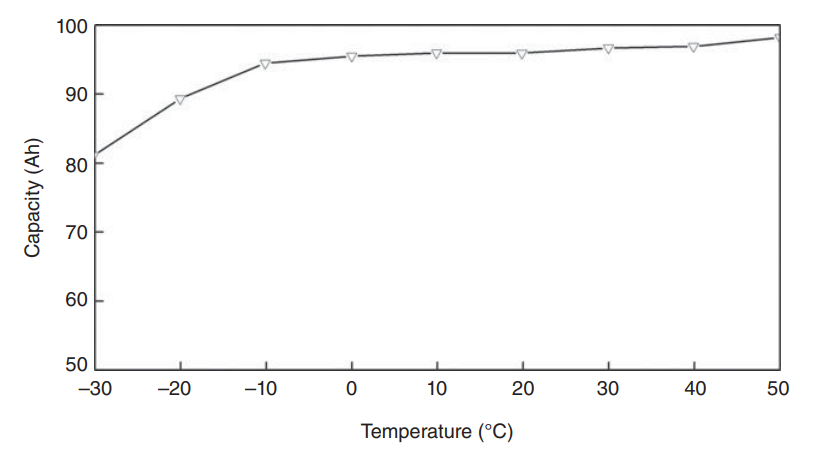
\includegraphics[width=0.6\linewidth]{Chapters/img/Current_vs_Temp.png}
			\centering
			\captionsetup{justification=centering,margin=2cm}
			\caption{กราฟแสดงความสัมพันธ์ระหว่างความจุกับอุณหภูมิ}
			\label{fig:Ah Vs Temp}
	\end{figure}
\end{center}
อุณหภูมิสูงมากจนเกินไปก็จะส่งผลเสียทำให้อายุการใช้งานของแบตเตอรี่นั้นสั้นลงและจะเห็นได้ว่าความสัมพันธ์ระหว่างอุณหภูมิกับความจุนั้นไม่เป็นเชิงเส้นดังนั้นเพื่อที่จะเพิ่มความแม่นยำในการประมาณค่า SOC มีความสำคัญอย่างมากที่จะต้องนำผลกระทบจากอุณภูมิมาทำการพิจารณาด้วย
%Table 6
\begin{center}
	\begin{figure}[H]
		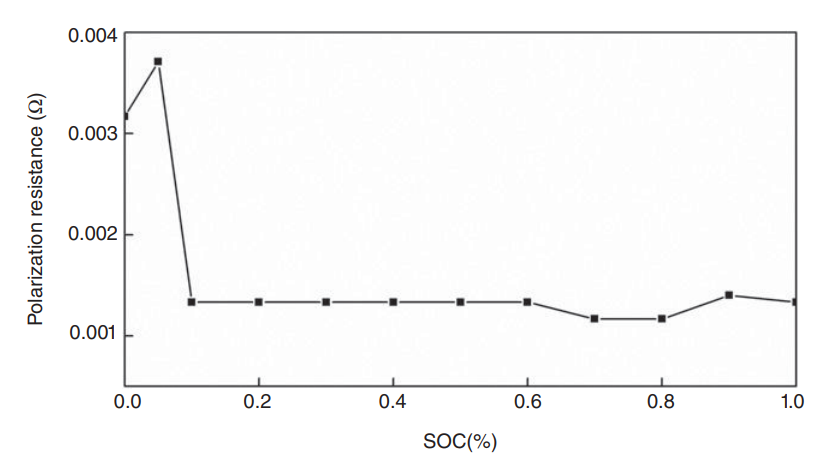
\includegraphics[width=0.6\linewidth]{Chapters/img/Pol_Resistance_vs_SOC.png}
			\centering
			\captionsetup{justification=centering,margin=2cm}
			\caption{กราฟแสดงความสัมพันธ์ระหว่างความต้านทานขั้วกับSOC}
	\end{figure}
\end{center}
%============================================================================================
\section{วงจรสมมูลของแบตเตอรี่}
	วงจรสมมูลสามารถใช้ในการจำลองคุณลักษณะต่างๆของแบตเตอรี่ระหว่างเงื่อนไขการทำงานต่างๆได้ซึ่งวงจรสมมูลของแบตเตอรี่ประกอบไปด้วยอุปกรณ์ทางไฟฟ้าต่างๆเช่น ตัวต้านทาน ตัวเก็บประจุ แหล่งจ่ายแรงดันไฟฟ้ากระแสตรง และอื่นๆ วงจรสมมูลนี้ถูกนำไปใช้ทั่วไปในการจำลองต้นแบบยานยนต์ไฟฟ้าและระบบการจัดการแบตเตอรี่ซึ่งในหัวข้อนี้จะยกตัวอย่างรูปแบบวงจรสมมูลที่เคยมีการใช้งานจริงอยู่ 4 วงจรคือ วงจรสมมูล Rint(Rint Model) วงจรสมมูลเทวินิน(Thevenin model) วงจรสมมูลRC(RC model) และวงจรสมมูลPNGV(PNGV model)ซึ่งแต่ละวงจรสมมูลมีความแตกต่างกันคือวงจรสมมูลเทวินินนั้นก็คือวงจรสมมูลRint ที่มีวงจรตัวต้านทานและตัวเก็บประจุขนานกันต่ออนุกรมเพิ่มเข้าไปเพื่อแทนคุณลักษณะที่เปลี่ยนแปลงของแบตเตอรี่ วงจรสมมูลPNGVนั้นก็คือวงจรสมมูลเทวินินที่เพิ่มตัวเก็บประจุ Cpb อนุกรมเข้าไปแทนแรงดันเปิดวงจรเทียบกับกระแสโหลด และสุดท้ายวงจรสมมูลRC นั้นมีความแตกต่างมากที่สุดเนื่องจากไม่มีแหล่งจ่ายแรงดันกระแสตรงอยู่ในวงจรเลย
\subsubsection*{วงจรสมมูลRint (Rint model)}
วงจรสมมูล Rint ถูกออกแบบโดยห้องปฏิบัติการแห่งชาติไอดาโฮ(The Idaho National Laboratory) ซึ่งประกอบไปด้วย
\begin{itemize}
{\item แหล่งจ่ายแรงดันไฟฟ้ากระแสตรงอุดมคติ Uocv แทนแรงดันเปิดวงจรของแบตเตอรี่}
{\item ตัวต้านทาน R แทนความต้านทานภายในของแบตเตอรี่}
\end{itemize}
\begin{center}
	\begin{figure}[H]
		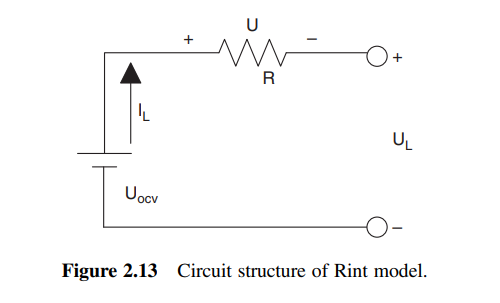
\includegraphics[width=0.6\linewidth]{Chapters/img/Rint_model.png}
			\centering
			\captionsetup{justification=centering,margin=2cm}
			\caption{วงจรสมมูลRint (Rint Model)}
	\end{figure}
\end{center}
ซึ่งแรงดันเปิดวงจรนั้นเป็นฟังก์ชั่นของ SOC และอุณหภูมิและค่าความต้านทานภายในนั้นเปลี่ยนแปลงเมื่อทำการชาร์จภายใต้ SOC ที่เท่ากัน
\subsubsection*{วงจรสมมูลเทวินิน (Thevenin model)}
วงจรสมมูลเทวินินเป็นวงจรสมมูลที่นิยมใช้กันมากที่สุดประกอบไปด้วย
\begin{itemize}
{\item 	แหล่งจ่ายแรงดันไฟฟ้ากระแสตรงอุดมคติ Uocv แทนแรงดันเปิดวงจรของแบตเตอรี่}
{\item 	ความต้านทาน Rohm แทนความต้านทานภายในของแบตเตอรี่}
{\item 	Rp และ Cp ที่ขนานกันแทนOverpotentialของแบตเตอรี่}
\end{itemize}
\begin{center}
	\begin{figure}[H]
		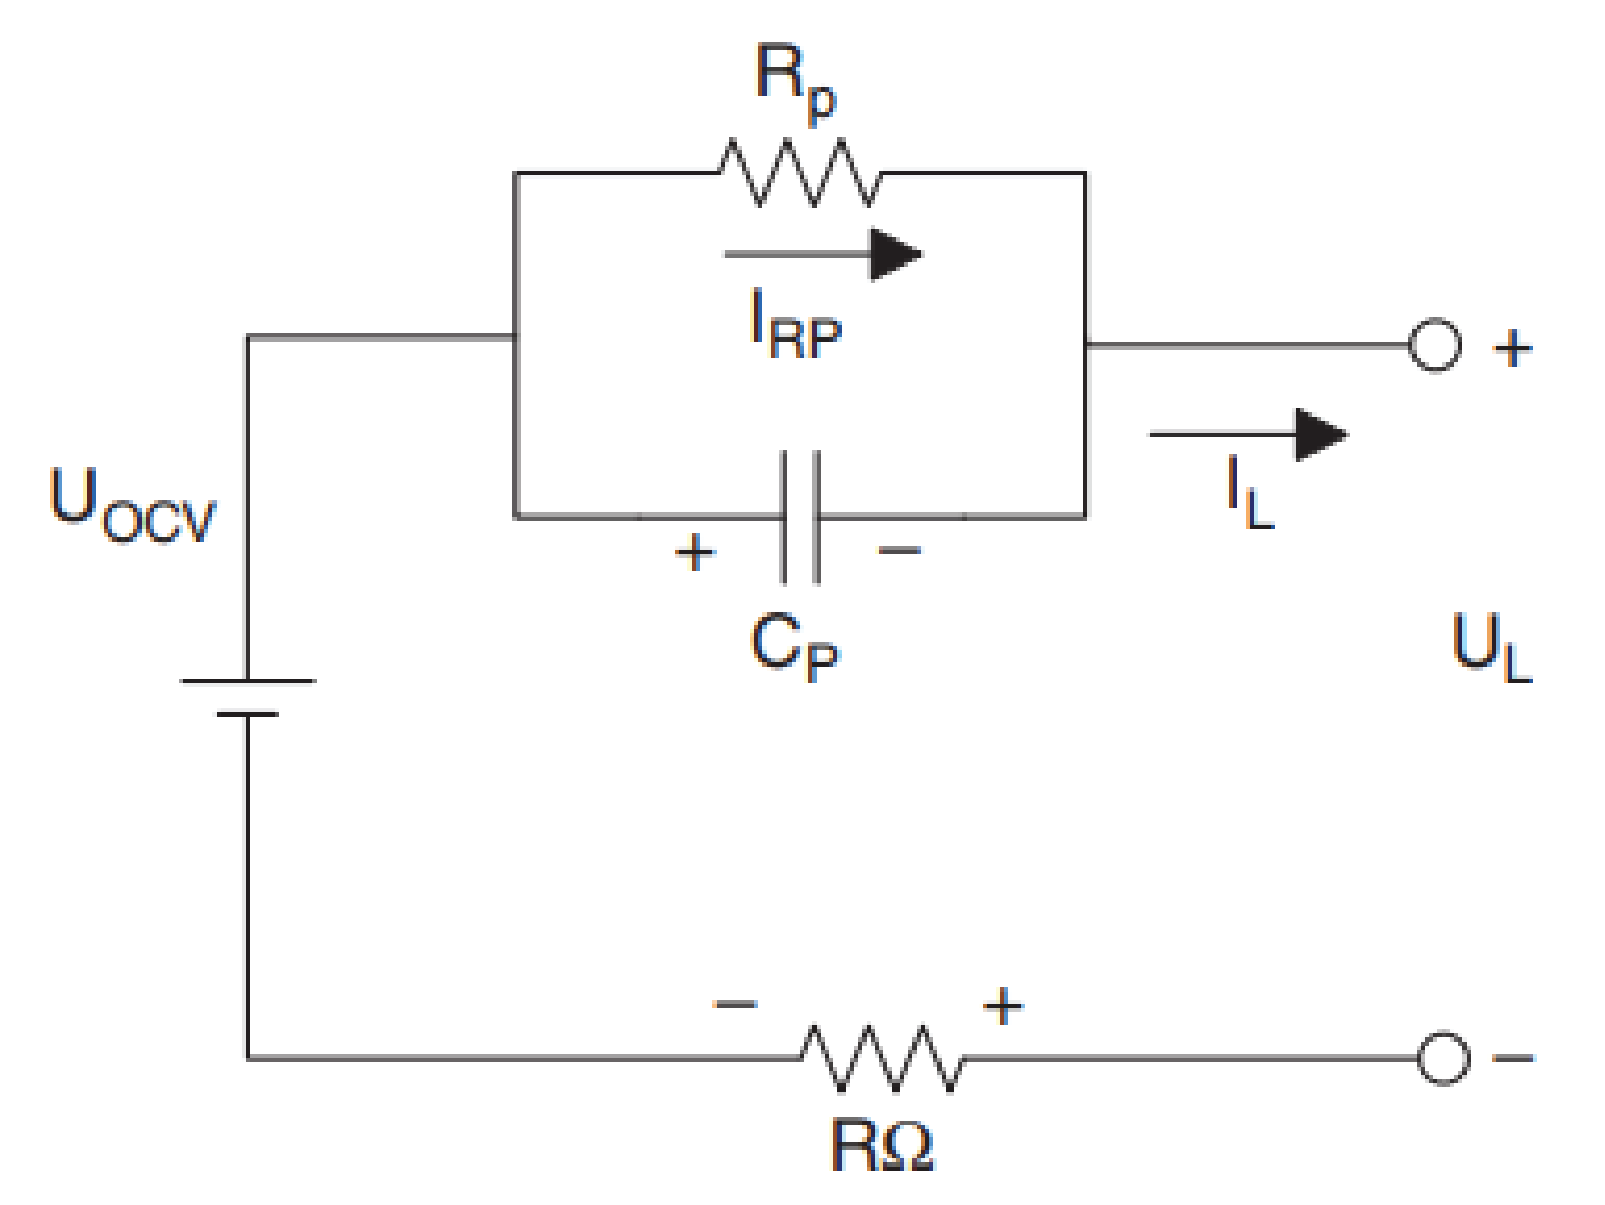
\includegraphics[width=0.6\linewidth]{Chapters/img/Thevenin_model.png}
			\centering
			\captionsetup{justification=centering,margin=2cm}
			\caption{วงจรสมมูลเทวินิน (Thevenin model)}
	\end{figure}
\end{center}
\subsubsection*{วงจรสมมูล RC (RC model)}
วงจรสมมูล RC มีตัวเก็บประจุ 2 ตัวและตัวต้านทาน 3 ตัวซึ่งถูกออกแบบโดยบริษัทผลิตแบตเตอรี่ SAFT ประกอบไปด้วย
\begin{itemize}
	{\item 	ตัวเก็บประจุ Cb แทนความจุในการเก็บพลังงาน(มีค่าขนาดใหญ่)}
	{\item 	ตัวเก็บประจุ Cc แทนผลกระทบจากพื้นผิวของอิเล็กโทรด}
	{\item 	ตัวต้านทาน Re แทนความต้านทานคัทออฟ(Cut-off resistance)}
	{\item 	ตัวต้านทาน Rc แทนความต้านทานของตัวเก็บประจุ(Capacitive resistance)}
\end{itemize}
โดยวงจรสมมูลนี้ขั้วแคโทดของแบตเตอรี่มีศักย์ไฟฟ้าเป็นศูนย์
\begin{center}
	\begin{figure}[H]
		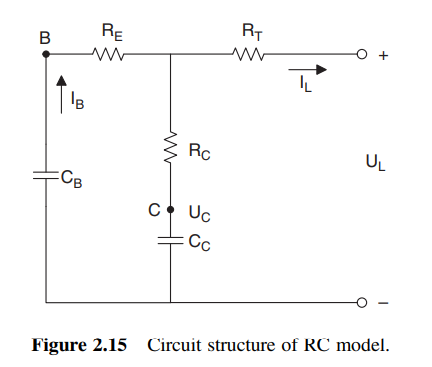
\includegraphics[width=0.6\linewidth]{Chapters/img/RC_model.png}
			\centering
			\captionsetup{justification=centering,margin=2cm}
			\caption{วงจรสมมูลRC (RC model)}
	\end{figure}
\end{center}
\subsubsection*{วงจรสมมูลPNGV (PNGV model)}
วงจรสมมูล PNGV เป็นวงจรสมมูลมาตรฐานที่ใช้ใน PNGV Battery Test Manual ในปี 2001 และใช้ใน Freedom CAR Battery Test Manual
 ในปี 2003 วงจรสมมูลนี้ประกอบไปด้วย
\begin{itemize}
	{\item 	แหล่งจ่ายแรงดันไฟฟ้ากระแสตรงอุดมคติ แทนแรงดันเปิดวงจรของแบตเตอรี่}
	{\item 	ตัวต้านทาน Rpo แทนความต้านทานภายในของแบตเตอรี่}
	{\item 	ตัวต้านทาน Rpp แทนความต้านทานที่ขั้วของแบตเตอรี่}
	{\item 	ตัวเก็บประจุ Cpp แทนความจุของขั้วแบตเตอรี่}
	{\item 	ตัวเก็บประจุ Cpb แทนแรงดันเปลี่ยนแปลงสะสมเทียบกับเวลาขณะต่อโหลด}
\end{itemize}
\begin{center}
	\begin{figure}[H]
		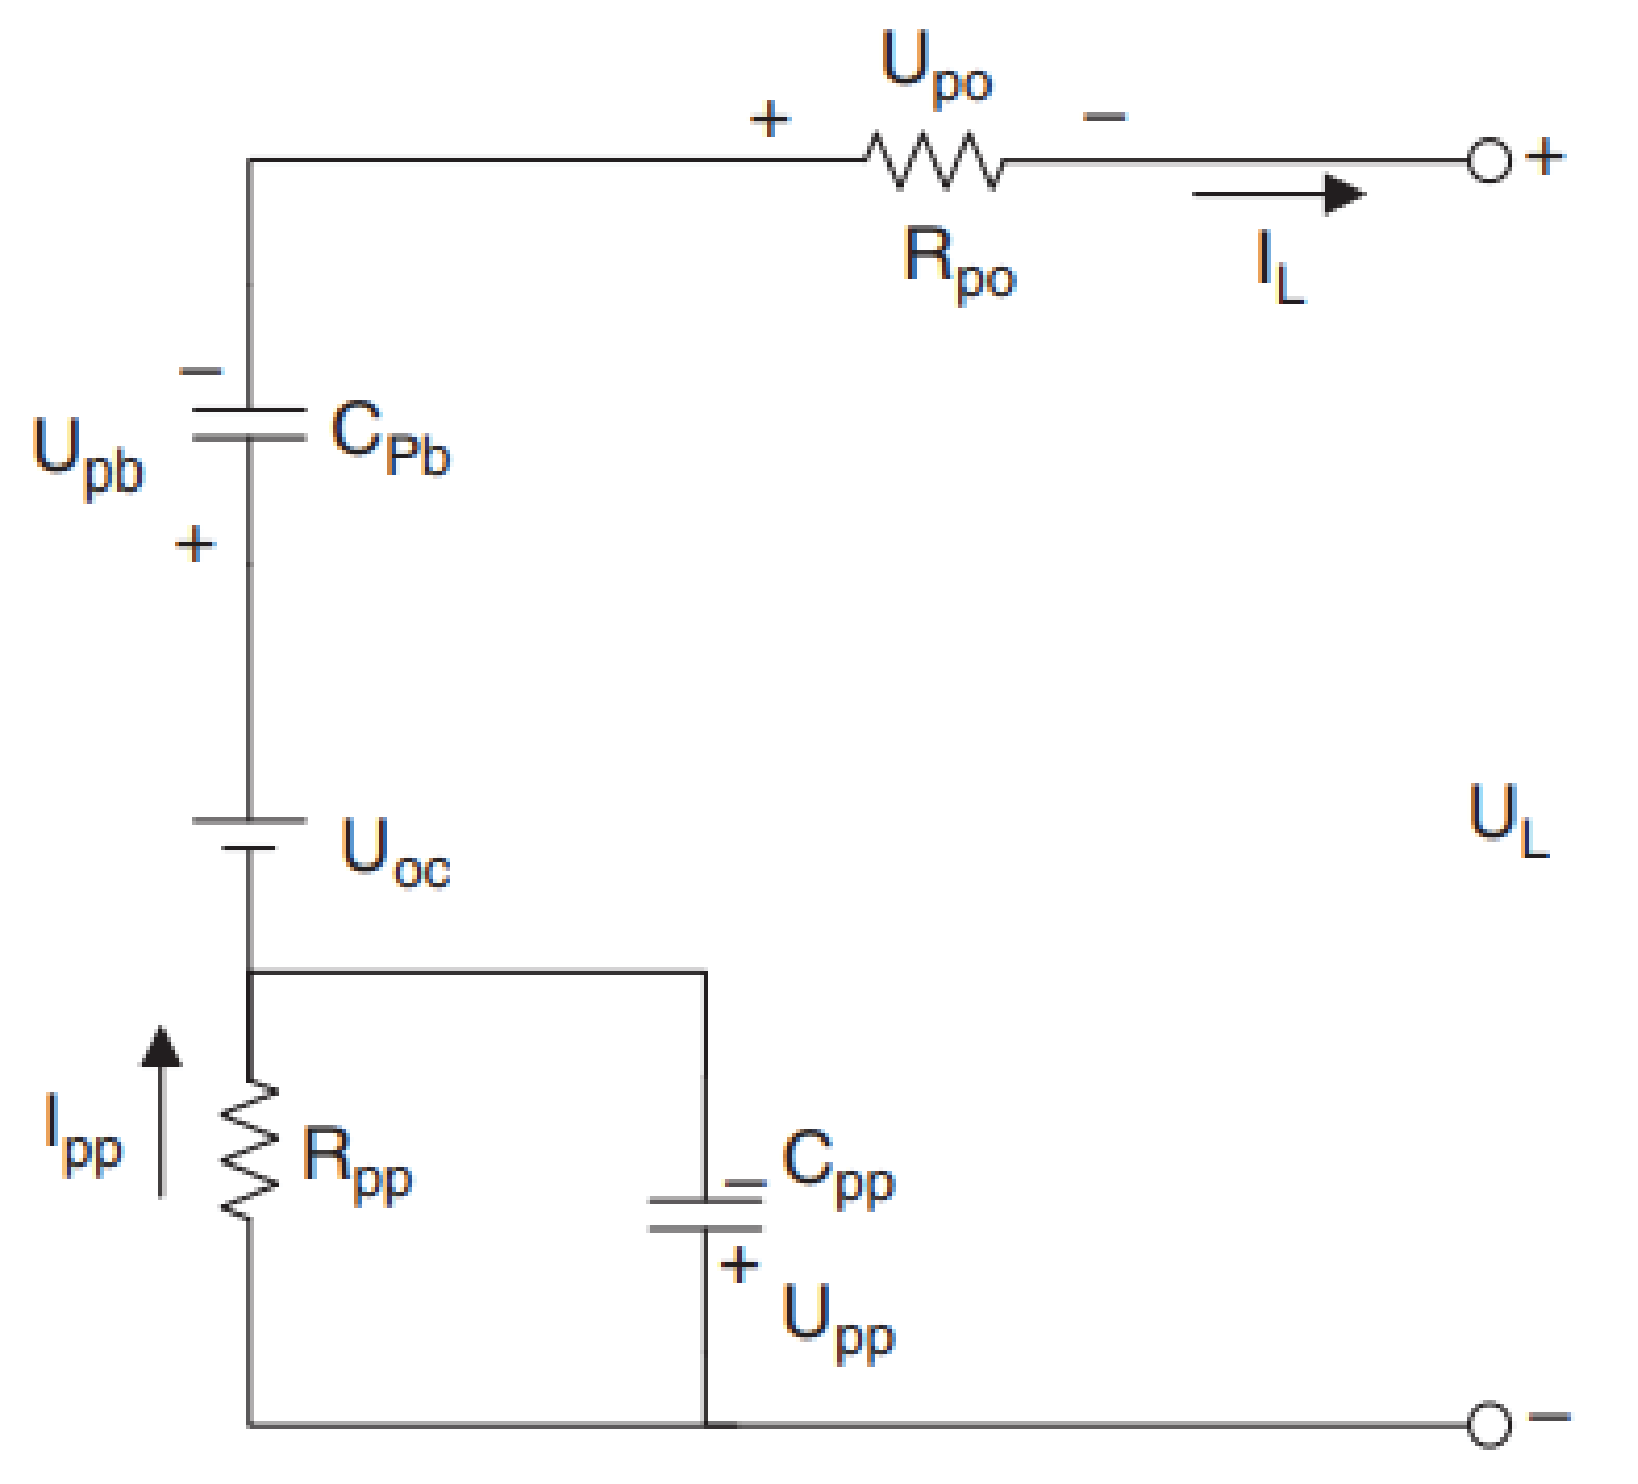
\includegraphics[width=0.6\linewidth]{Chapters/img/PNGV_model.png}
			\centering
			\captionsetup{justification=centering,margin=2cm}
			\caption{วงจรสมมูลPNGV (PNGV model)}
	\end{figure}
\end{center}
%===============================================================================
\section{ระบบการจัดการแบตเตอรี่(BMS)}
ระบบการจัดการแบตเตอรี่คือระบบอิเล็กทรอนิกส์ที่ใช้ในการจัดการแบตเตอรี่ปฐมภูมิ เช่น ปกป้องแบตเตอรี่จากปัจจัยต่างๆที่ทำให้แบตเตอรี่ทำงานในช่วงการทำงานที่ไม่ปลอดภัยหรือการทำงานที่อาจจะเกิดความเสียหายต่อแบตเตอรี่ 
วัดและควบคุมสภาพของแบตเตอรี่ คำนวณข้อมูลทุติย-ภูมิรายงานข้อมูลนั้นเป็นต้น
สำหรับยานยนต์ไฟฟ้าระบบการจัดการแบตเตอรี่มีความสำคัญอย่างมากกับความปลอดภัย เพิ่มประสิทธิภาพระบบของยานยนต์ไฟฟ้า และลดค่าใช้จ่ายในการซ่อมแซมซึ่งระบบการจัดการแบตเตอรี่นั้นต้องสามารถตรวจจับสภาพของแบตเตอรี่และค้นหาสาเหตุของความบกพร่องได้อย่างทันทีและส่งข้อไปยังหน่วยควบคุมยานยนต์(Vehicle Control Unit, VCU)หรือส่งข้อมูลไปยังอุปกรณ์ควบคุมการชาร์จ(Charger)เพื่อให้หน่วยควบคุมยานยนต์หรืออุปกรณ์ควบคุมการชาร์จจะสามารถเลือกวิธีที่จะต้องตอบสนองและประยุกต์ใช้งานแบตเตอรี่ได้อย่างปลอดภัยและมีประสิทธิภาพมากที่สุด
\subsection{การทำงานของระบบการจัดการแบตเตอรี่}
การทำงานของระบบการจัดการแบตเตอรี่นั้นสารมารถทำได้หลายอย่างมากโดยระบบการจัดการแบตเตอรี่นั้นขึ้นอยู่กับการออกแบบให้สามารถทำงานได้ตามที่ต้องการดังนั้นระบบการจัดการแบตเตอรี่แต่ละระบบจึงมีการทำงานที่แตกต่างกันไปขึ้น
อยู่กับการนำไปประยุกต์ใช้ในงานต่างๆ ขนาด ต้นทุนในการผลิตและอื่นๆ โดยในหัวข้อนี้จะกล่าวถึงการทำงานที่ระบบการจัดการแบตเตอรี่ส่วนมากสามารถทำได้ดังนี้
\subsubsection*{การตรวจจับหรือการวัดของระบบการจัดการแบตเตอรี่}
ระบบการจัดการแบตเตอรี่จะตรวจจับหรือทำการวัดค่าต่างๆดังเช่น
\begin{itemize}
	{\item 	แรงดัน เช่น แรงดันรวมของแบตเตอรี่ แรงดันในแต่ละเซลล์ของแบตเตอรี่}
	{\item 	อุณหภูมิ เช่น อุณหภูมิเฉลี่ย อุณหภูมิก่อนระบายความร้อน อุณหภูมิหลังระบายความร้อน อุณหภูมิของแต่ละเซลล์แบตเตอรี่}
	{\item 	กระแสไฟฟ้า เช่น กระแสไฟฟ้าที่ไหลเข้าและออกจากแบตเตอรี่}
\end{itemize}
\subsubsection*{การป้องกันของระบบการจัดการแบตเตอรี่}
ระบบการจัดการแบตเตอรี่สามารถหลีกเลี่ยงหรือป้องกันปัจจัยต่างๆที่ทำให้ส่งผลเสียต่อแบตเตอรี่ได้ดังเช่น
\begin{itemize}
	{\item 	กระแสไฟฟ้าเกินจากการชาร์จและดิสชาร์จ}
	{\item 	แรงดันไฟฟ้าเกินระหว่างการชาร์จและดิสชาร์จ}
	{\item 	อุณหภูมิที่สูงเกินไปและต่ำเกินไป}
	{\item 	กระแสไฟฟ้ารั่วไหล}
	{\item 	การสลับขั้วกรณีที่มีการต่อวงจรผิดและการลัดวงจร}
	{\item 	การปรับสมดุลแบตเตอรี่ของระบบการจัดการแบตเตอรี่}
\end{itemize}
\subsubsection*{การคำนวณต่างๆของระบบการจัดการแบตเตอรี่}
ระบบการจัดการแบตเตอรี่สามารถคำนวณค่าต่างๆได้ดังเช่น
\begin{itemize}
	{\item 	แรงดัน เช่น แรงดันต่ำสุดและสูงสุดของเซลล์แบตเตอรี่}
	{\item 	State of charge(SOC)}
	{\item 	Depth of discharge(DOD)}
	{\item 	State of health(SOH)}
	{\item 	State of power(SOP)}
	{\item 	อิมพีแดนซ์ภายในเซลล์แบตเตอรี่}
	{\item 	จำนวนครั้งการชารา์จและดิสชาร์จ}
\end{itemize}
\subsubsection*{การติดต่อสื่อสารของระบบการจัดการแบตเตอรี่}
ระบบการจัดการแบตเตอรี่ขนาดเล็กอาจจะไม่มีการติดต่อส่งข้อมูลให้กับอุปกรณ์ภายนอกหรืออุปกรณ์ภายในระบบแต่ระบบการจัดการแบตเตอรี่หลายระบบที่มีขนาดใหญ่และมีความซับซ้อนมากขึ้นเช่น
ระบบการจัดการแบตเตอรี่ของยานยนต์ไฟฟ้านั้นหน่วยประมวลผลของระบบการจัดการแบตเตอรี่สามารถติดต่อส่งข้อมูลให้กับอุปกรณ์ภายนอกหรือสามามารถส่งข้อมูลภายในระบบหรืออาจจะติดต่อส่งข้อมูล
ได้ทั้งอุปกณ์ภายในและภายนอกระบบ\newline\hspace*{2cm}
สำหรับการส่งข้อมูลให้กับอุปกรณ์ภายนอกระบบดังเช่น
\begin{itemize}
	{\item 	การสื่อสารแบบอนุกรม(Serial communications)}
	{\item 	CAN bus communications โดยส่วนมากการส่งข้อมูลด้วยวิธีนี้ใช้กับยานยนต์}
	{\item 	การสื่อสารแบบไร้สาย(Wireless communications)}
\end{itemize}
สำหรับการส่งข้อมูลกันภายในระบบดังเช่น
\begin{itemize}
	{\item 	Isolated serial communications}
	{\item 	Wireless serial communications}
\end{itemize}

































\chapter{ขั้นตอนวิธีการทดสอบแบตเตอรี่ตามมาตรฐาน}
แบตเตอรี่เป็นส่วนประกอบที่มีความสำคัญมากสำหรับยานยนต์ไฟฟ้าเนื่องจากเป็นอุปกรณ์ที่กักเก็บและให้พลังงานไฟฟ้ากับยานยนต์ไฟฟ้าเพื่อความปลอดภัยของผู้ที่ใช้งานยานยนต์ไฟฟ้ามาต-รฐานต่างๆจึงถูกกำหนดขึ้นเพื่อ
ใช้กับทุกส่วนประกอบของยานยนต์ไฟฟ้ารวมถึงแบตเตอรี่ด้วยเช่นกันซึ่งการทดสอบแบตเตอรี่ที่ทางคณะผู้จัดทำได้ทำการทดสอบนั้นจะทดสอบตามมาตรฐาน UN ECE Regulation 136 ทั้งหมด 2 หัวข้อดังนี้
%\subsection{การทดสอบการป้องกันการลัดวงจรภายนอกของแบตเตอรี่}
%ในหัวข้อนี้จะเป็นการทดสอบการป้องกันการลัดวงจรภายนอกแบตเตอรี่ของแบตเตอรี่โดยจุดประสงค์ของการทดสอบนี้เพื่อทดสอบความสามารถการป้องกันการลัดวงจรของแบตเตอรี่โดยถ้าแบตเตอรี่มีอุปกรณ์ป้องกันการลัดวงจรอยู่ภาย
%ในดังนั้นอุปกรณ์ป้องกันการลัดวงจรนี้ต้องขัดจังหวะหรือจำกัดกระแสลัดวงจรเพื่อป้องกันความเสียหายที่จะเกิดขึ้นจากการลัดวงจรของแบตเตอรี่
%\newline
%\newline
%\textbf{เงื่อนไขทั่วไปในขั้นตอนการทดสอบ}
%\begin{itemize}
%{\item ระหว่างการทดสอบแบตเตอรี่ต้องทำงานอยู่ในอุณหภูมิ 20$\pm$10$^{\circ}C$ หรือสูงกว่า}
%{\item ก่อนการทดสอบแบตเตอรี่ต้องมีระดับ SOC มากกว่า 50\% ของช่วง SOC ที่แบตเตอรี่อยู่ในสภาวะการทำงานปกติ}
%{\item เมื่อเริ่มทำการทดสอบอุปกรณ์ป้องกันทุกอย่างที่ส่งผลต่อการทำงานของแบตเตอรี่ซึ่งให้ผลลัพธ์ตามจุดประสงค์ของการทดสอบจะต้องทำงาน}
%\end{itemize}
%\textbf{ขั้นตอนการทดสอบการลัดวงจร}
%\begin{itemize}
%{\item ขั้นแรกสวิตซ์ตัวนำต่างๆที่ใช้สำหรับการชาร์จและดิสชาร์จต้องปิดวงจรเพื่อจำลองถึงการใช้งานแบตเตอรี่ขณะขับขี่ยานยนต์ไฟฟ้าและการชาร์จแบตเตอรี่ภายนอกยานยนต์ไฟฟ้าถ้าหากขั้นตอนนี้ไม่สำเร็จให้ทำขั้นตอนนี้อีกครั้งจนกว่าจะสำเร็จ}
%{\item ขั้วบวกและขั้วลบของแบตเตอรี่จะต้องทำการเชื่อมต่อถึงกันและกันเพื่อให้เกิดการลัดวงจรโดยอุปกรณ์การเชื่อมต่อนี้จะต้องมีความต้านทานไม่เกิน 5 มิลลิโอห์ม}
%{\item การลัดวงจรจะถูกดำเนินไปอย่างต่อเนื่องจนกว่าจะถูกขัดจังหวะจากการทำงานของแบตเตอรี่หรือมีการจำกัดกระแสลัดวงจร หรือต้องมีการวัดอุณหภูมิที่ตัวแบตเตอรี่เป็นเวลาอย่างน้อย 1 ชั่วโมงโดยตลอดระยะเวลาที่ทำการวัดอุณหภูมิต้องมีการเปลี่นแปลงไม่เกิน 4$^{\circ}C$}
%{\item การทดสอบจะยุติลงหลังจากการสังเกตการแบตเตอรี่ที่อุณหภูมิตามเงื่อนไขข้างต้นตามสภาพแวดล้อมที่ใช้ในการทดสอบ}
%\end{itemize}
%=======================================================================================================
\subsection{การทดสอบการป้องกันการชาร์จเกินของแบตเตอรี่}
สำหรับหัวข้อการทดสอบนี้จะเป็นการทดสอบการป้องกันการชาร์จไฟฟ้าเกินขีดจำกัดของแบตเตอรี่เพื่อเป็นการทดสอบประสิทธิภาพการป้องกันการชาร์จเกินขีดจำกัดของแบตเตอรี่
\newline
\newline
\textbf{เงื่อนไขทั่วไปในขั้นตอนการทดสอบ}
\begin{itemize}
{\item ระหว่างการทดสอบแบตเตอรี่ต้องทำงานอยู่ในอุณหภูมิ 20$\pm$10$^{\circ}C$ หรือสูงกว่า}
{\item เมื่อเริ่มทำการทดสอบอุปกรณ์ป้องกันทุกอย่างที่ส่งผลต่อการทำงานของแบตเตอรี่ซึ่งให้ผลลัพธ์ตามจุดประสงค์ของการทดสอบจะต้องทำงาน}
\end{itemize}
\textbf{ขั้นตอนการทดสอบการชาร์จ}
\begin{itemize}
{\item ขั้นแรกสวิตซ์ตัวนำต่างๆที่ใช้สำหรับการชาร์จต้องปิดวงจร}
{\item อุปกรณ์ควบคุมจำกัดการชาร์จของอุปกรณ์วัดหรืออุปกรณ์ทดสอบแบตเตอรี่ต้องถูกปิดการใช้งาน}
{\item แบตเตอรี่ต้องถูกชาร์จด้วยอัตรากระแสอย่างน้อย 1/3 C แต่ต้องไม่เกินกระแสสูงสุดในช่วงการทำงานปกติตามที่ผู้ผลิตแบตเตอรี่ได้กำหนดไว้}
{\item การชาร์จจะถูกดำเนินไปอย่างต่อเนื่องจนกว่าการชาร์จจะถูกขัดจังหวะจากการทำงานของแบตเตอรี่หรือการชาร์จถึงขีดจำกัด เมื่อการขัดจังหวะโดยการทำงานของแบตเตอรี่นั้นไม่ทำงานหรือตัวแบตเตอรี่ไม่มีการทำงานในส่วนของการขัดจังหวะนี้การชาร์จจะถูกดำเนินต่อไปเรื่อยๆจนกว่าจะชาร์จถึง 2 เท่าของความจุพิกัด}
{\item การทดสอบจะยุติลงหลังจากการสังเกตการแบตเตอรี่ที่อุณหภูมิตามเงื่อนไขข้างต้นตามสภาพแวดล้อมที่ใช้ในการทดสอบ}
\end{itemize}
%=======================================================================================================
\subsection{การทดสอบการป้องกันการดิสชาร์จเกินของแบตเตอรี่}
ในการทดสอบการป้องกันการดิสชาร์จเกินโดยวัตถุประสงค์ของการทดสอบนี้เพื่อทดสอบความสามารถในการป้องกันการดิสชาร์จเกินของแบตเตอรี่โดยถ้าแบตเตอรี่มีอุปกรณ์ป้องกันการชาร์จเกินอยู่ภายในดังนั้นอุปกรณ์ป้องกันการชาร์จเกิน
นี้ต้องขัดจังหวะหรือจำกัดกระแสการดิสชาร์จเพื่อป้องกันความเสียหายต่างๆเนื่องจากค่า SOC ที่ต่ำเกินกว่าที่ผู้ผลิตแบตเตอรี่ได้กำหนดเอาไว้
\newline
\newline
\textbf{เงื่อนไขทั่วไปในขั้นตอนการทดสอบ}
\begin{itemize}
{\item ระหว่างการทดสอบแบตเตอรี่ต้องทำงานอยู่ในอุณหภูมิ 20$\pm$10$^{\circ}C$ หรือสูงกว่า}
{\item เมื่อเริ่มทำการทดสอบอุปกรณ์ป้องกันทุกอย่างที่ส่งผลต่อการทำงานของแบตเตอรี่ซึ่งให้ผลลัพธ์ตามจุดประสงค์ของการทดสอบจะต้องทำงาน}
\end{itemize}
\textbf{ขั้นตอนการทดสอบการดิสชาร์จ}
\begin{itemize}
{\item ขั้นแรกสวิตซ์ตัวนำต่างๆที่ใช้สำหรับการดิสชาร์จต้องปิดวงจร}
{\item อุปกรณ์ควบคุมจำกัดการชาร์จของอุปกรณ์วัดหรืออุปกรณ์ทดสอบแบตเตอรี่ต้องถูกปิดการใช้งาน}
{\item แบตเตอรี่ต้องถูกดิสชาร์จด้วยอัตรากระแสอย่างน้อย 1/3 C แต่ต้องไม่เกินกระแสสูงสุดในช่วงการทำงานปกติตามที่ผู้ผลิตแบตเตอรี่ได้กำหนดไว้}
{\item การดิสชาร์จจะถูกดำเนินไปอย่างต่อเนื่องจนกว่าการดิสชาร์จจะถูกขัดจังหวะจากการทำงานของแบตเตอรี่หรือการดิสชาร์จถึงขีดจำกัด เมื่อการขัดจังหวะโดยการทำงานของแบตเตอรี่นั้นไม่ทำงานหรือตัวแบตเตอรี่ไม่มีการทำงานในส่วนของการขัดจังหวะนี้การดิสชาร์จจะถูกดำเนินต่อไปเรื่อยๆจนกว่าแบตเตอรี่จะถูกดิสชาร์จจนถึง 25\% ของระดับแรงดันปกติ}
{\item หลังหยุดการดิสชาร์จแล้วแบตเตอรี่จะต้องนำไปชาร์จใหม่ด้วยอัตรากระแสปกติตามที่ผู้ผลิตได้กำหนดไว้ถ้าหากไม่ได้มีการกำหนดจะต้องทำการชาร์จด้วยอัตรากระแส 1/3 C}
{\item การทดสอบจะยุติลงหลังจากการสังเกตการแบตเตอรี่ที่อุณหภูมิตามเงื่อนไขข้างต้นตามสภาพแวดล้อมที่ใช้ในการทดสอบ}
\end{itemize}
%========================================================================================================
โดยทั้ง 2 หัวข้อของการทดสอบตามมาตรฐาน UN ECE Regulation 136 นั้นเงื่อนไขที่จะผ่านการทดสอบแบตเตอรี่มีดังนี้
\begin{enumerate}
{\item ในระหว่างการทดสอบแบตเตอรี่จะต้องไม่มีอิเล็กโทรไลต์รั่วไหลออกจากแบตเตอรี่ โดยการสังเกตการรั่วไหลของอิเล็กโทรไลต์ให้สังเกตโดยรอบของแบตเตอรี่เพียงเท่านั้นโดยไม่ต้องแยกชิ้นส่วนใดๆของแบตเตอรี่ออก}
{\item ในระหว่างการทดสอบแบตเตอรี่จะต้องไม่เกิดการแตกหักหรือฉีกขาด}
{\item ในระหว่างการทดสอบแบตเตอรี่จะต้องไม่เกิดเพลิงไหม้}
{\item ในระหว่างการทดสอบแบตเตอรี่จะต้องไม่เกิดการระเบิด}
\end{enumerate}
%========================================================================================================
\section{ขั้นตอนการทดสอบอื่นๆ}
สำหรับการทดสอบอื่นที่นอกเหนือจากทดสอบตามาตรฐานนี้จะทดสอบด้วยกันทั้งหมด 3 หัวข้อคือ
\begin{itemize}
{\item การทดสอบระยะเวลาในการพัก}
{\item การทดสอบอัตรากระแส}
{\item การทดสอบการวัดค่าความต้านทานภายในของโมดูลแบตเตอรี่}
\end{itemize}
\subsection{การทดสอบระยะเวลาในการพักของแบตเตอรี่}
สำหรับการทดสอบนี้จะทดสอบเพื่อหาระยะเวลาในการพักแบตเตอรี่ที่เหมาะสมที่สุดที่แบตเตอรี่จะไม่เกิดการเปลี่ยนแปลงโดยขั้นตอนการทดสอบมีดังนี้
\begin{enumerate}
{\item ทำการชาร์จแบตเตอรี่ด้วยวิธีกระแสงที่แรงดันคงที่(CC-CV) จนกระทั้งแรงดันถึง 80\%SOC}
{\item เมื่อชาร์จแบตเตอรี่แล้วทำการพักเพื่อสังเกต 3 ชั่วโมง}
{\item ทำการดิสชาร์จด้วยวิธีกระแสคงที่(CC) จนกระทั่งแรงดันถึง 20\%SOC}
{\item เมื่อดิสชาร์จแบตเตอรี่แล้วทำการพักเพื่อสังเกต 3 ชั่วโมง}
\end{enumerate}
\subsection{การทดสอบอัตรากระแส}
สำหรับการทดสอบนี้จะทดสอบเพื่อศึกษาอัตรากระแสนั้นมีผลต่อแรงดันและความจุอย่างไร
\begin{enumerate}
{\item ทำการชาร์จแบตเตอรี่ด้วยวิธีกระแสงที่แรงดันคงที่(CC-CV) จนกระทั้งแรงดันถึง 80\%SOC}
{\item เมื่อชาร์จแบตเตอรี่แล้วทำการพัก 30 นาที}
{\item ทำการดิสชาร์จด้วยวิธีกระแสคงที่(CC) จนกระทั่งแรงดันถึง 20\%SOC}
{\item เมื่อดิสชาร์จแบตเตอรี่แล้วทำการพักเพื่อสังเกต 30 นาที}
{\item ทำซ้ำตั้งแต่ขั้นตอนแรก}
\end{enumerate}
โดยจะทดสอบทั้งหมดตามขั้นตอนนี้ 3 ครั้งโดยแต่ละครั้งจะเปลี่ยนอัตรากระแสการดิสชาร์จคือ 0.2C 0.3C และ 0.5C
\subsection{การทดสอบวัดค่าความต้านทานภายในของแบตเตอรี่}
การทดสอบนี้จะเป็นการทดสอบการวัดค่าความต้านทานภายในของแบตเตอรี่ด้วยไฟฟ้ากระแสตรง(Direct Current Internal Resistance,DCIR)
จากมาตรฐาน IEC61960 ขั้นตอนการทดสอบคือ
\begin{enumerate}
{\item ดิสชาร์จด้วยกระแสคงที่ 0.2C เป็นระยะเวลา 10 วินาที}
{\item ดิสชาร์จด้วยกระแสคงที่ 1C เป็นระยะเวลา 1 วินาที}
\end{enumerate}
จากนั้นสังเกตและบันทึกค่าแรงดันที่เปลี่ยนแปลงต่ออัตรากระแสที่เปลี่ยนแปลงจากนั้นนำมาวิเคราะห์ดังสมการ
$ DCIR = \frac{V_2-V_1}{I_1-I_2} $
%========================================================================================================
\section{อุปกรณ์สำหรับทดสอบแบตเตอรี่}
ในการทดสอบแบตเตอรี่สำหรับโครงงานนี้อุปกรณ์หลักที่จะใช้ในการทดสอบในหัวข้อต่างๆคือเครื่องทดสอบแบตเตอรี่ Chroma Model 17020 โดยอุปกรณ์ที่ใช้ในระบบของเครื่องนี้ประกอบด้วย
\begin{enumerate}
{\item 69200-1 Charge/Discharge Controller \newline
ทำหน้าที่เก็บข้อมูลการทดสอบแบตเตอรี่ทุกๆ 1 วินาทีและสามารถควบคุมการทำงานผ่านระบบอีเทอร์เน็ต(Ethernet)ได้}
{\item A691101 DC/AC Bi-Direction Converter\newline
ทำหน้าที่แปลงกระแสไฟฟ้าเป็นไฟฟ้ากระแสตรงให้กับเครื่องทดสอบและสามารถแปลงกระแสไฟฟ้ากระแสตรงจากแบตเตอรี่ให้เป็นกระแสสลับเพื่อนำกลับมาใช้ใหม่}
{\item 69225-100-4 Regenerative Charge/Discharge Tester\newline
ทำหน้าที่จ่ายพลังงานไฟฟ้าให้กับแบตเตอรี่หรือรับพลังงานไฟฟ้าจากแบตเตอรี่}
{\item ON/OFF Controller\newline
ทำหน้าที่ควบคุมการจ่ายพลังงานไฟฟ้าให้กับระบบของเครื่องทดสอบแบตเตอรี่}
\end{enumerate}
\begin{center}
	\begin{figure}[H]
		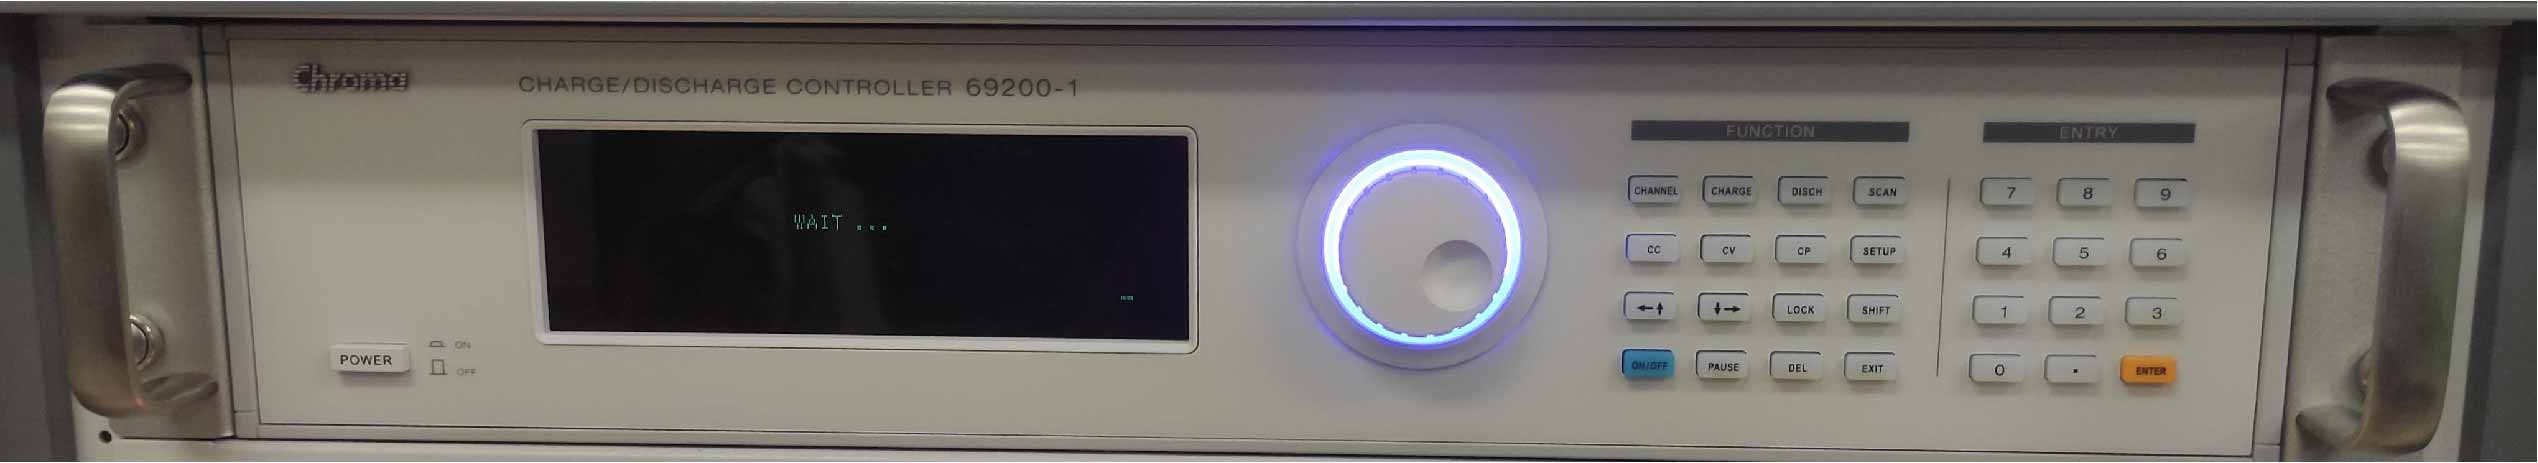
\includegraphics[width=1\linewidth]{Chapters/img/Charge_Discharge_Controller.jpg}
			\centering
			\captionsetup{justification=centering,margin=2cm}
			\caption{Charge/Discharge Controller}
	\end{figure}
	\begin{figure}[H]
		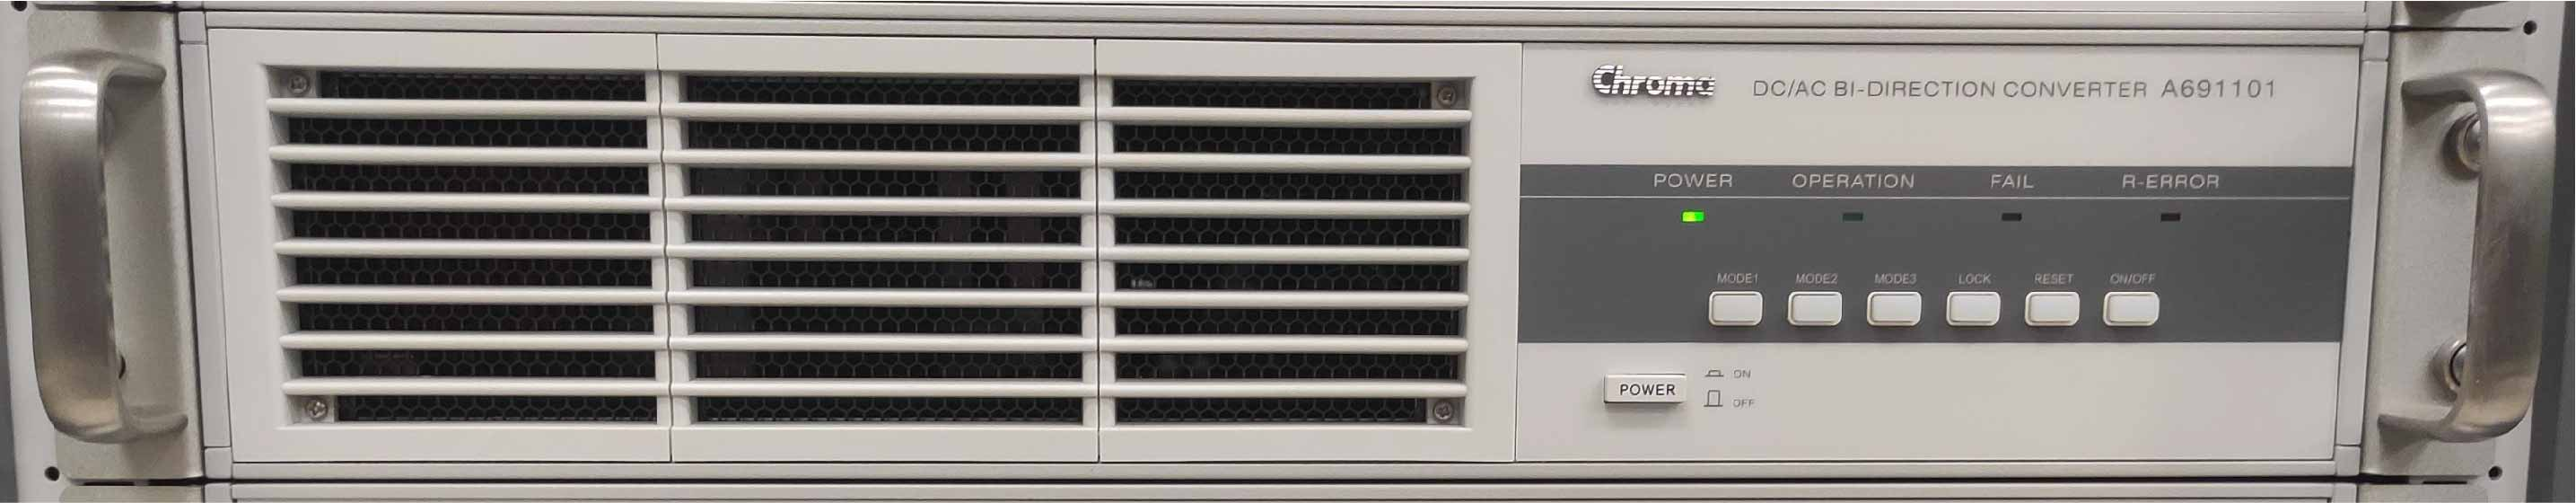
\includegraphics[width=1\linewidth]{Chapters/img/Bi_Direction_Converter.jpg}
			\centering
			\captionsetup{justification=centering,margin=2cm}
			\caption{DC/AC Bi-Direction Converter}
	\end{figure}
	\begin{figure}[H]
		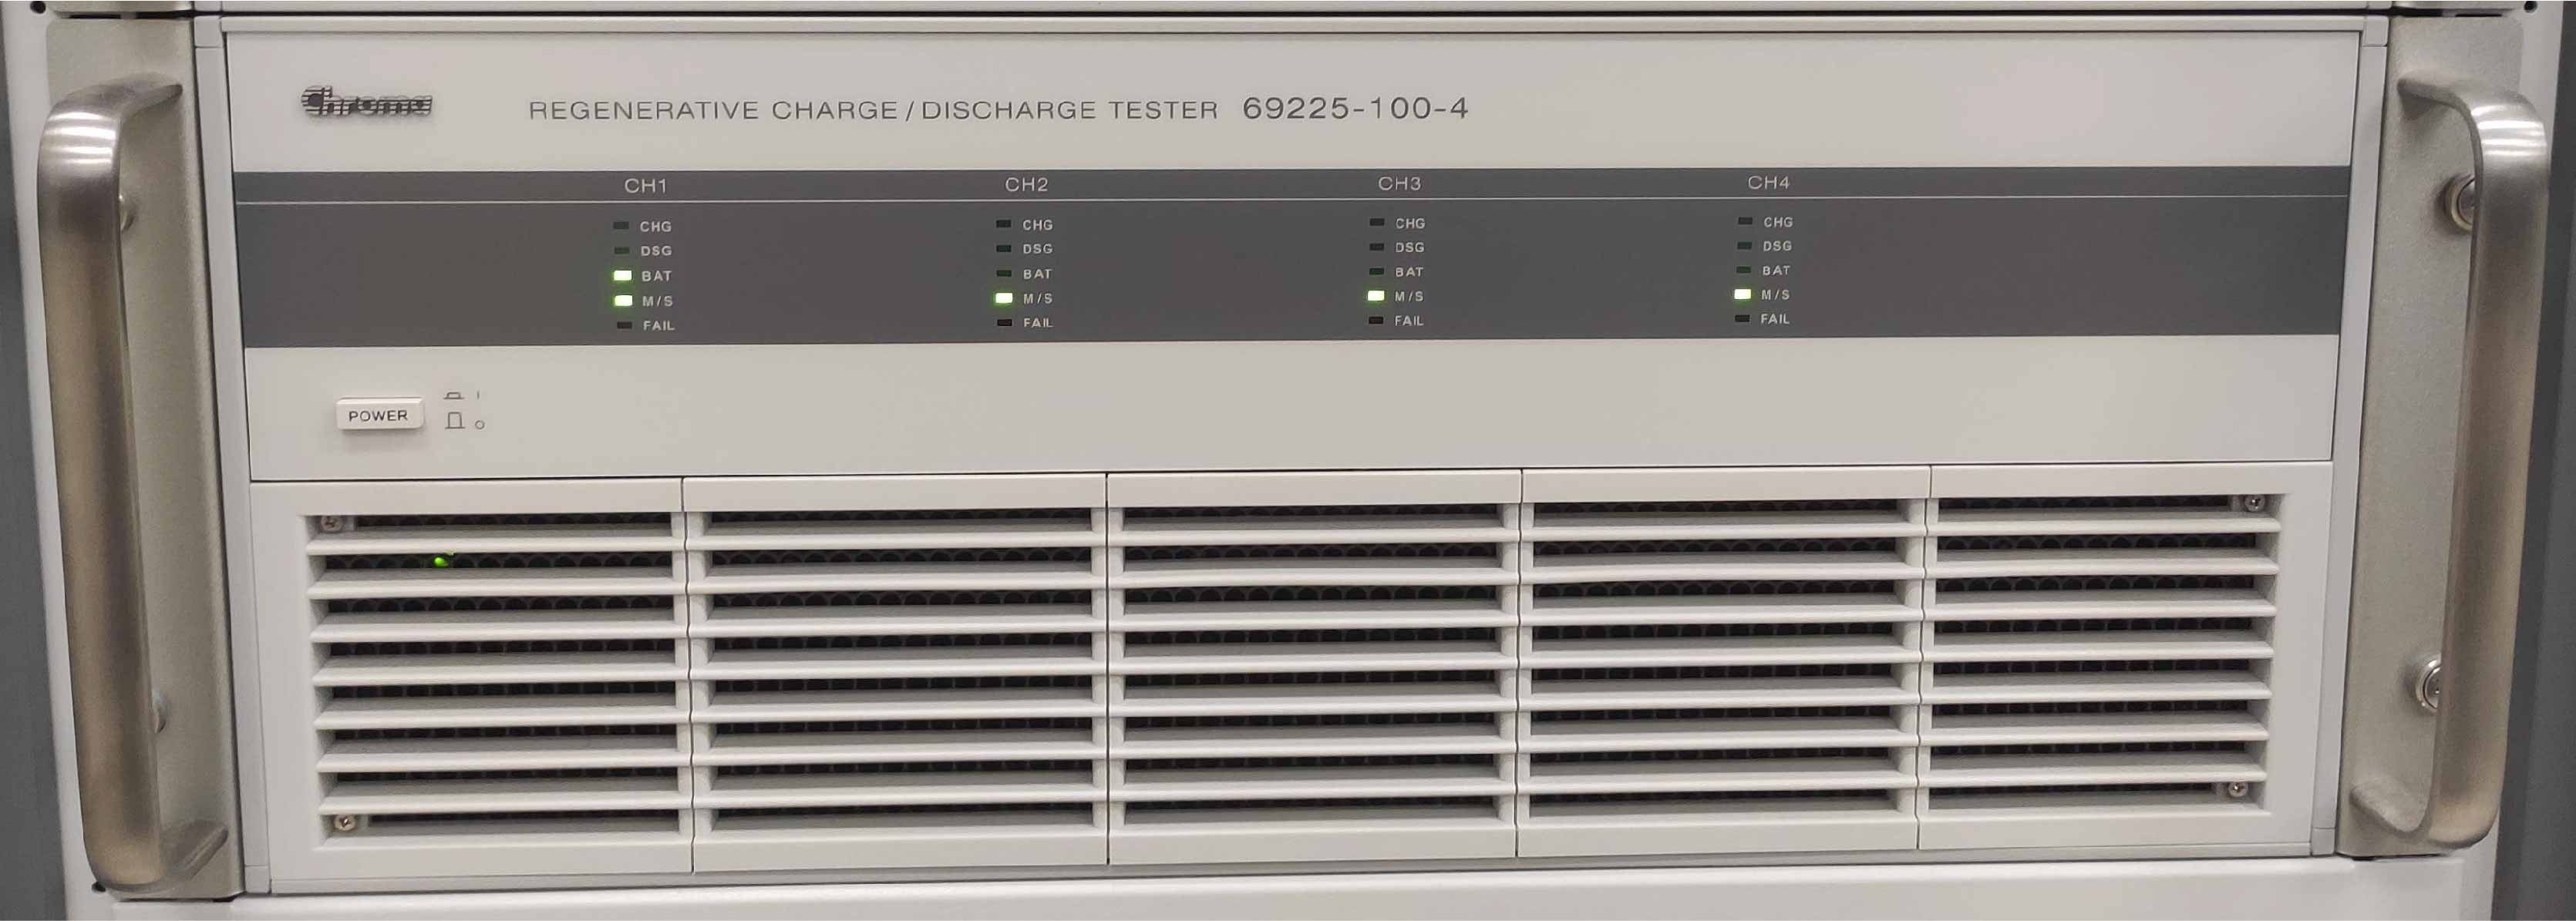
\includegraphics[width=1\linewidth]{Chapters/img/Regenerative_Charge_Discharge.jpg}
			\centering
			\captionsetup{justification=centering,margin=2cm}
			\caption{Regenerative Charge/Discharge Tester}
	\end{figure}
	\begin{figure}[H]
		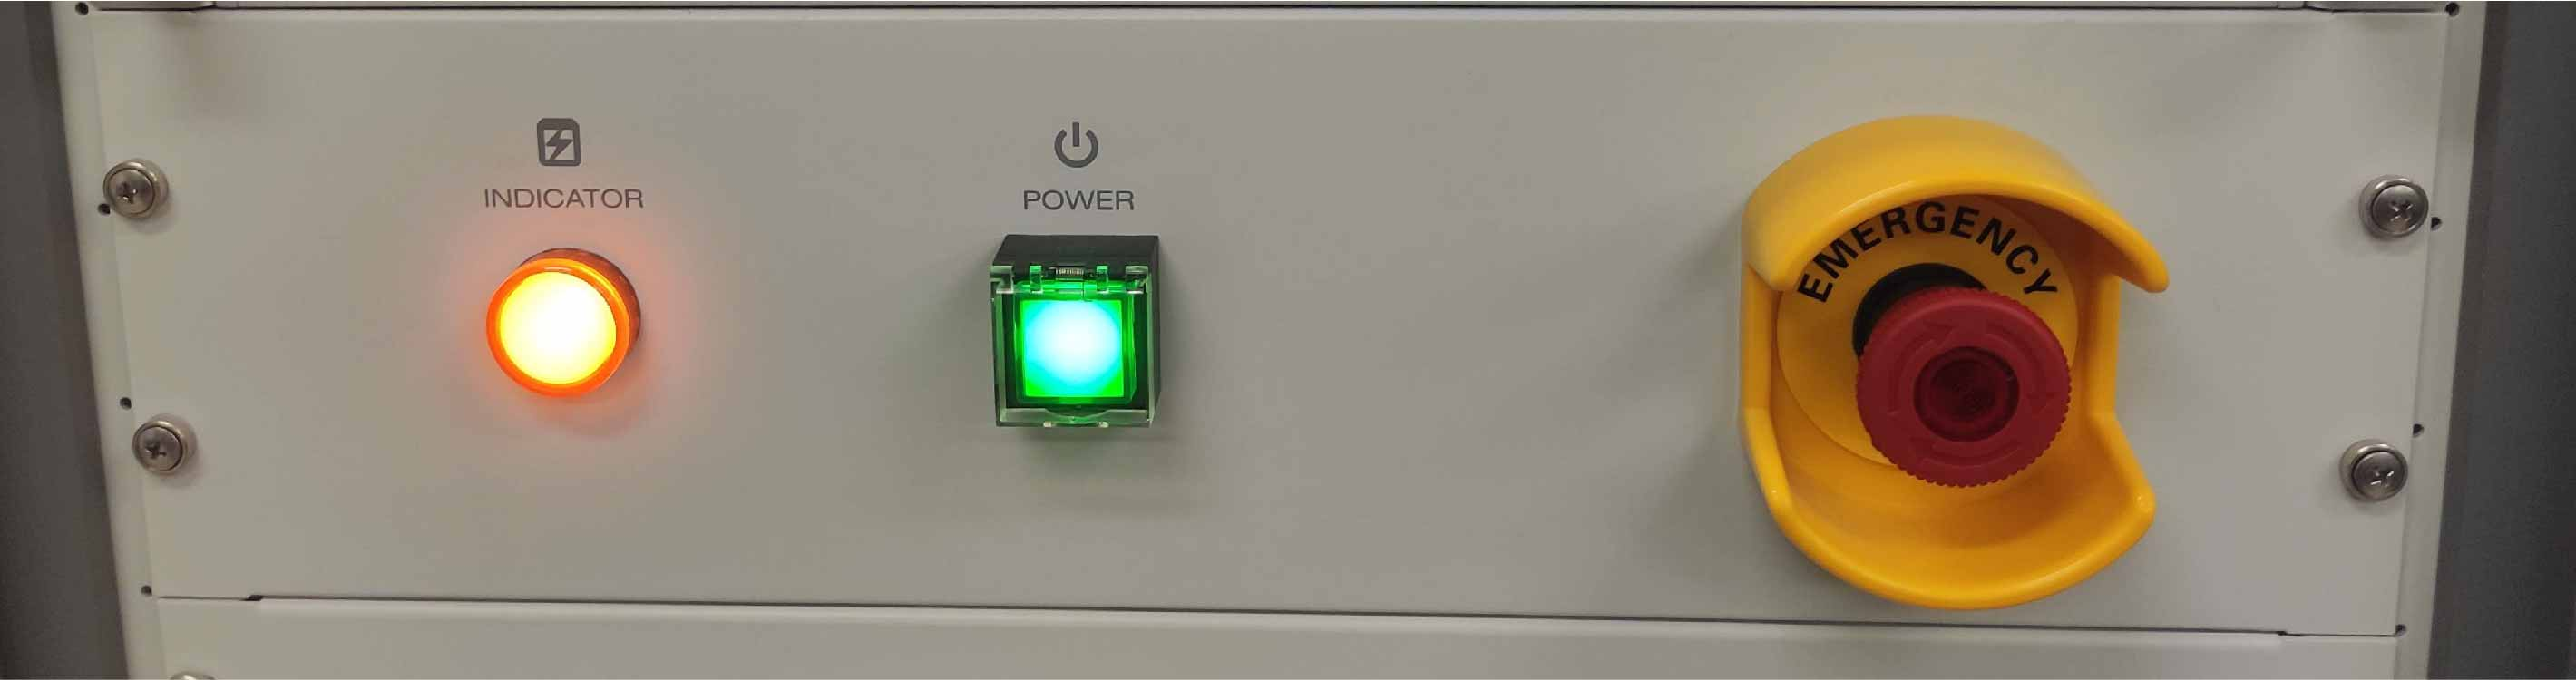
\includegraphics[width=1\linewidth]{Chapters/img/ON_OFF_Controller.jpg}
			\centering
			\captionsetup{justification=centering,margin=2cm}
			\caption{ON/OFF Controller}
	\end{figure}
%	\begin{figure}[!h]
%		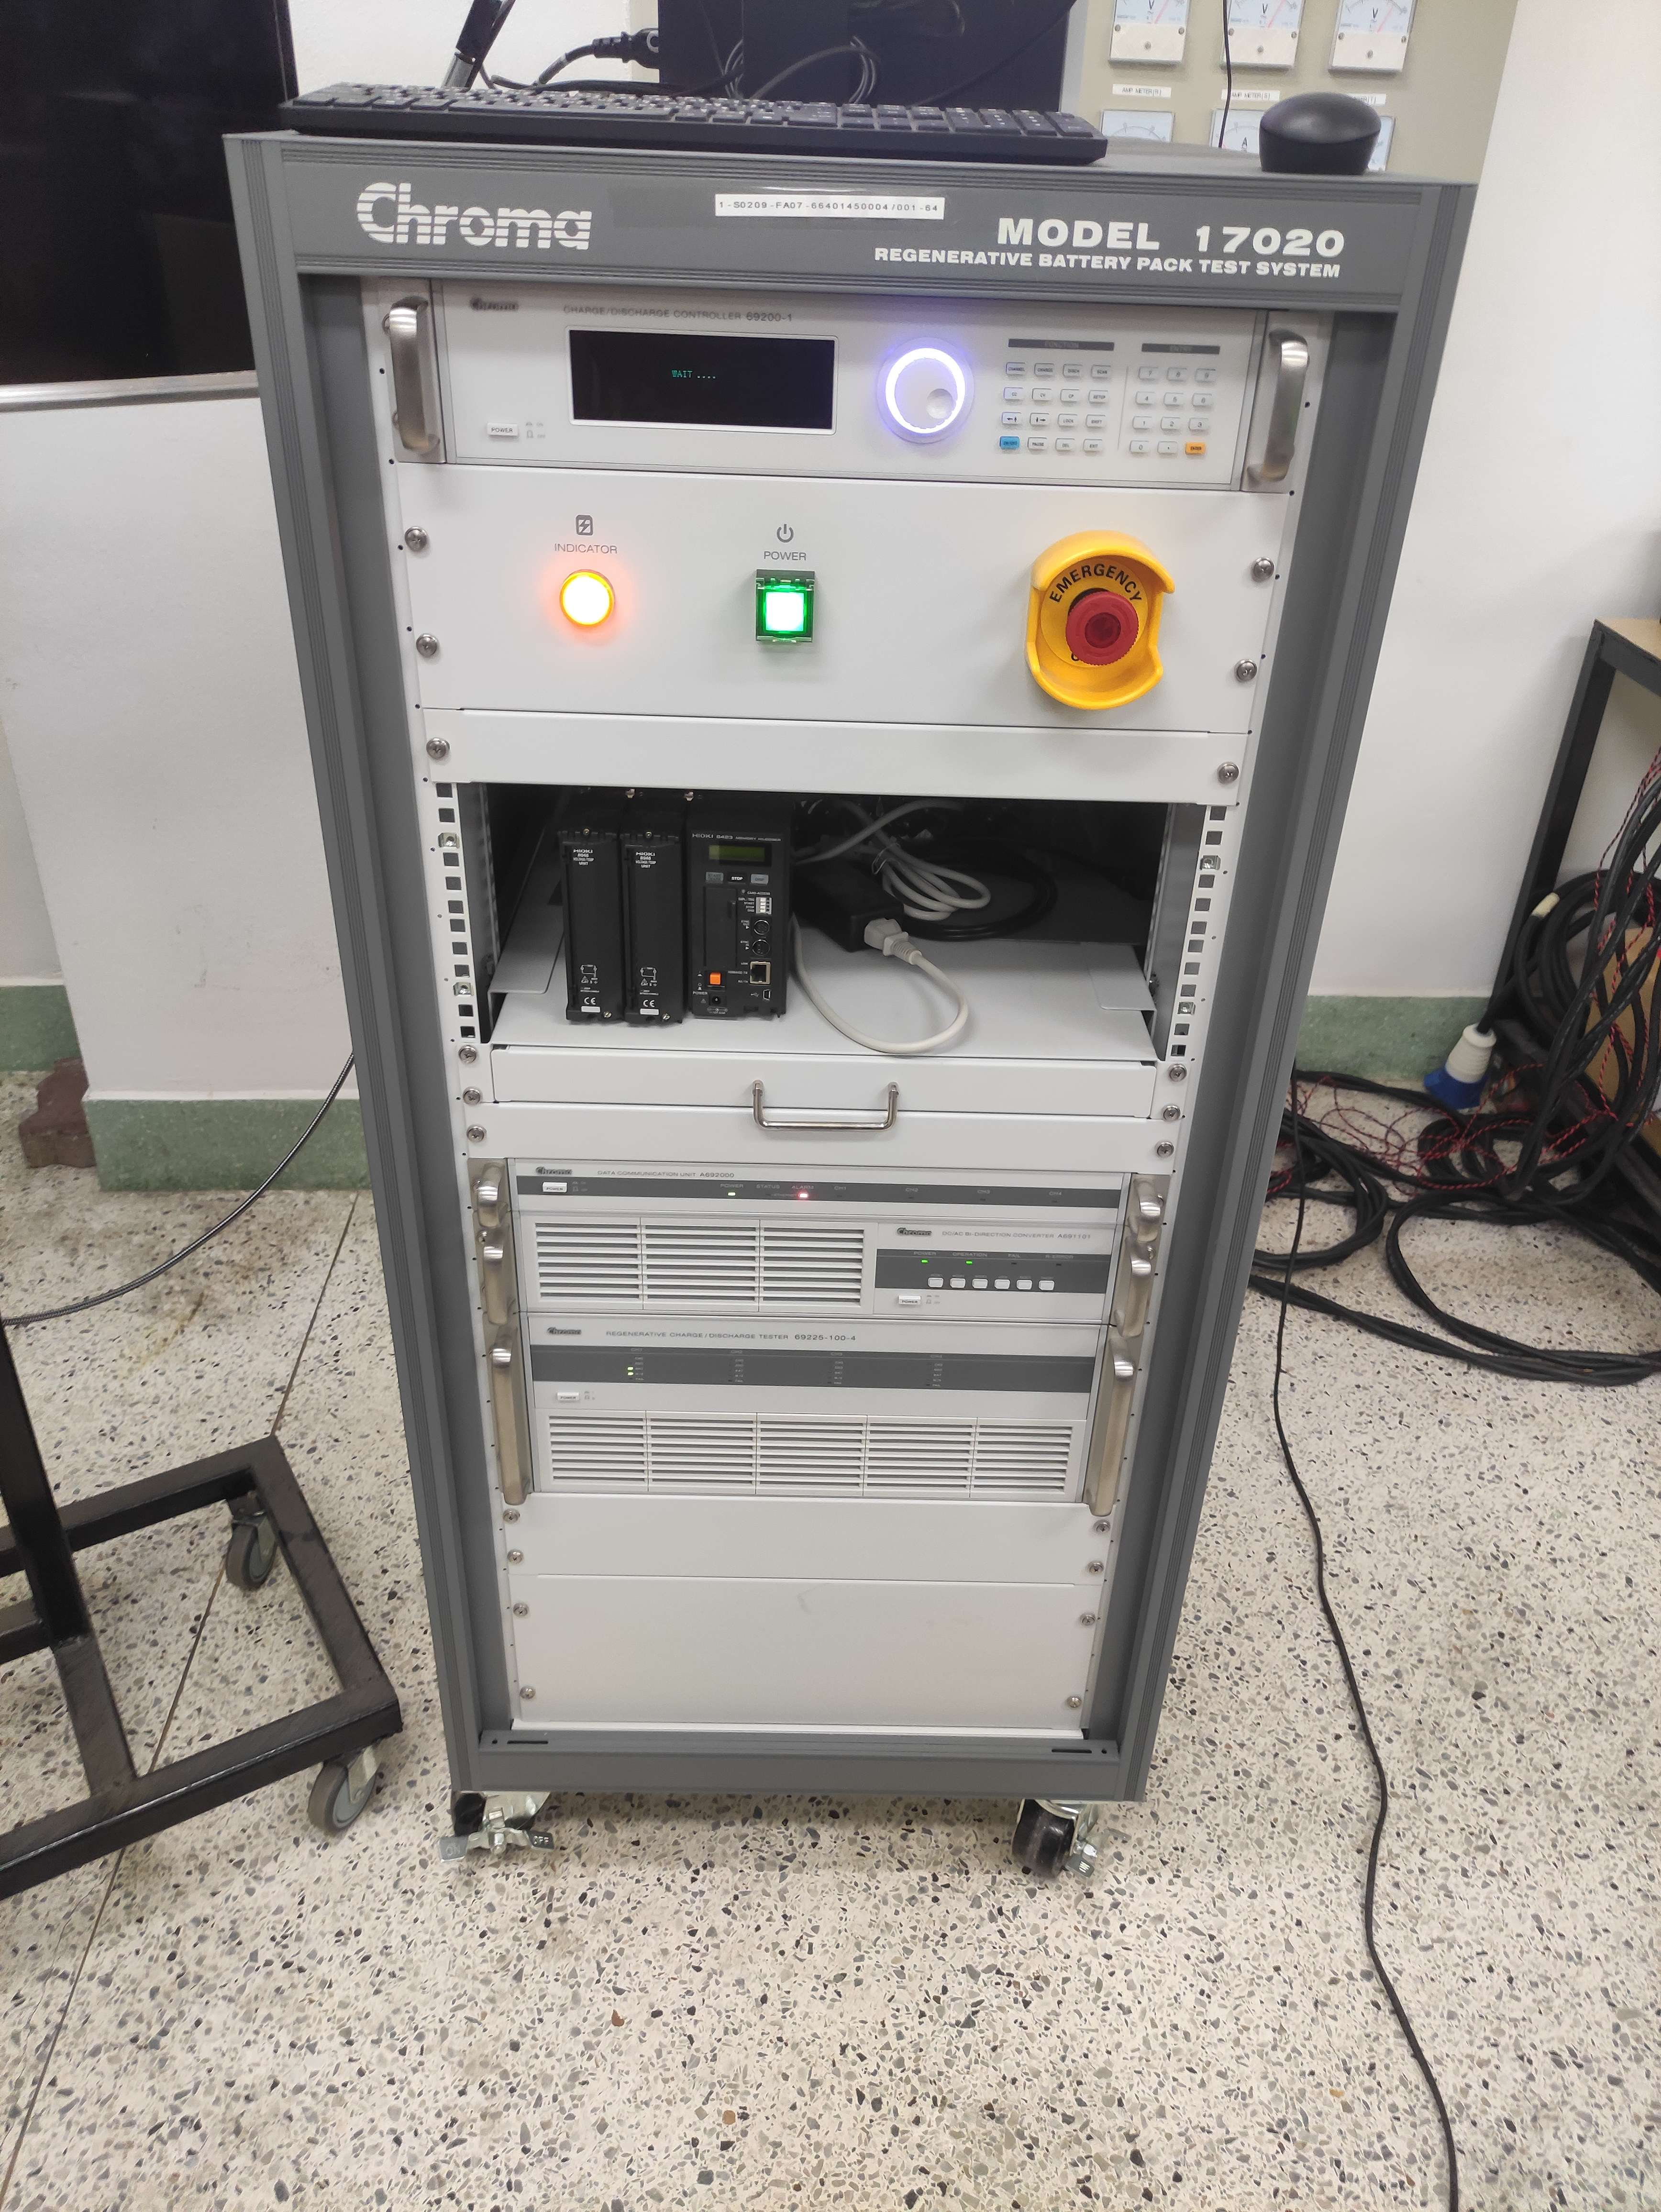
\includegraphics[width=0.5\linewidth]{Chapters/img/Chroma_17020_3.jpg}
%			\centering
%			\captionsetup{justification=centering,margin=2cm}
%			\caption{เครื่องทดสอบแบตเตอรี่ Chroma Model 17020}
%	\end{figure}
\begin{figure}[!h]
	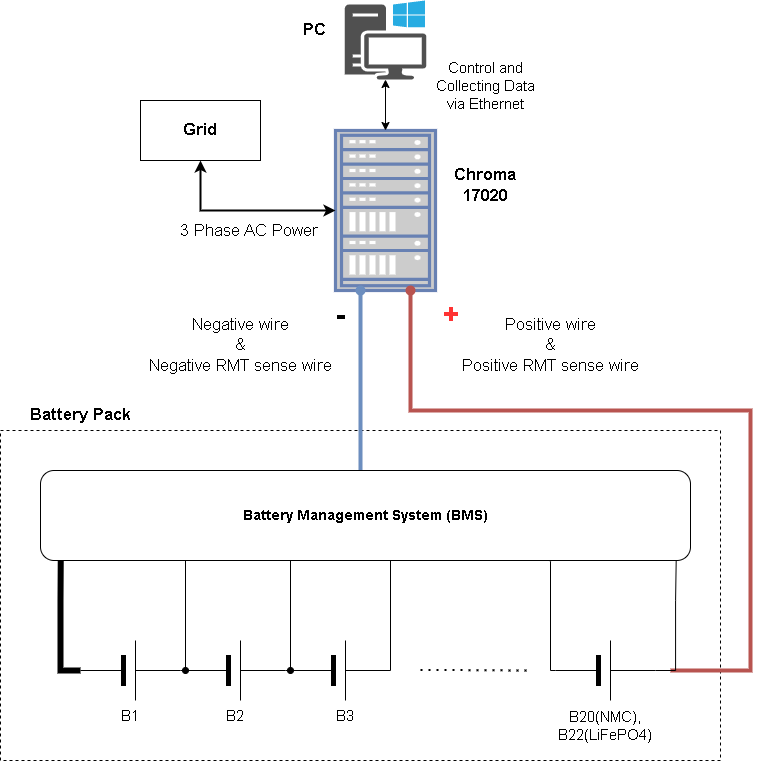
\includegraphics[width=1\linewidth]{Chapters/img/Testing_System.png}
		\centering
		\captionsetup{justification=centering,margin=2cm}
		\caption{แผนภาพระบบการทดสอบแบตเตอรี่}
	\end{figure}
\end{center}
%========================================================================
\vfill
\subsection{แบตเตอรี่สำหรับทำการทดสอบ}
แบตเตอรี่ที่ทำการทดสอบเป็นแบตเตอรี่ชนิดลิเธียมแมงกานีสโคบอลท์ออกไซด์(NMC)พิกัด 72V/30Ah ซึ่งคุณสมบัติแสดงดังตาราง
\begin{center}
	\begin{figure}[H]
		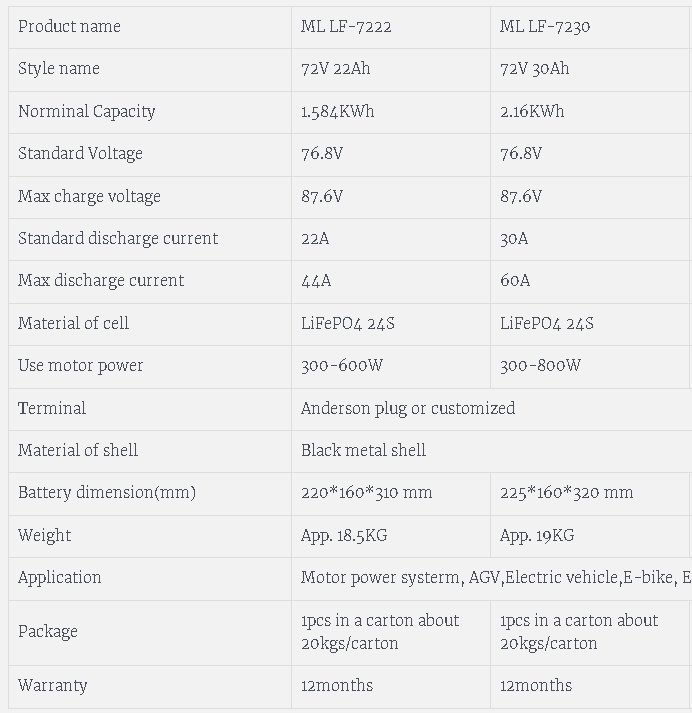
\includegraphics[width=0.5\linewidth]{Chapters/img/Battery_name_plate.PNG}
		\centering
		\captionsetup{justification=centering,margin=2cm}
		\caption{ตารางคุณสมบัติของแบตเตอรี่}
	\end{figure}
	\begin{figure}[H]
		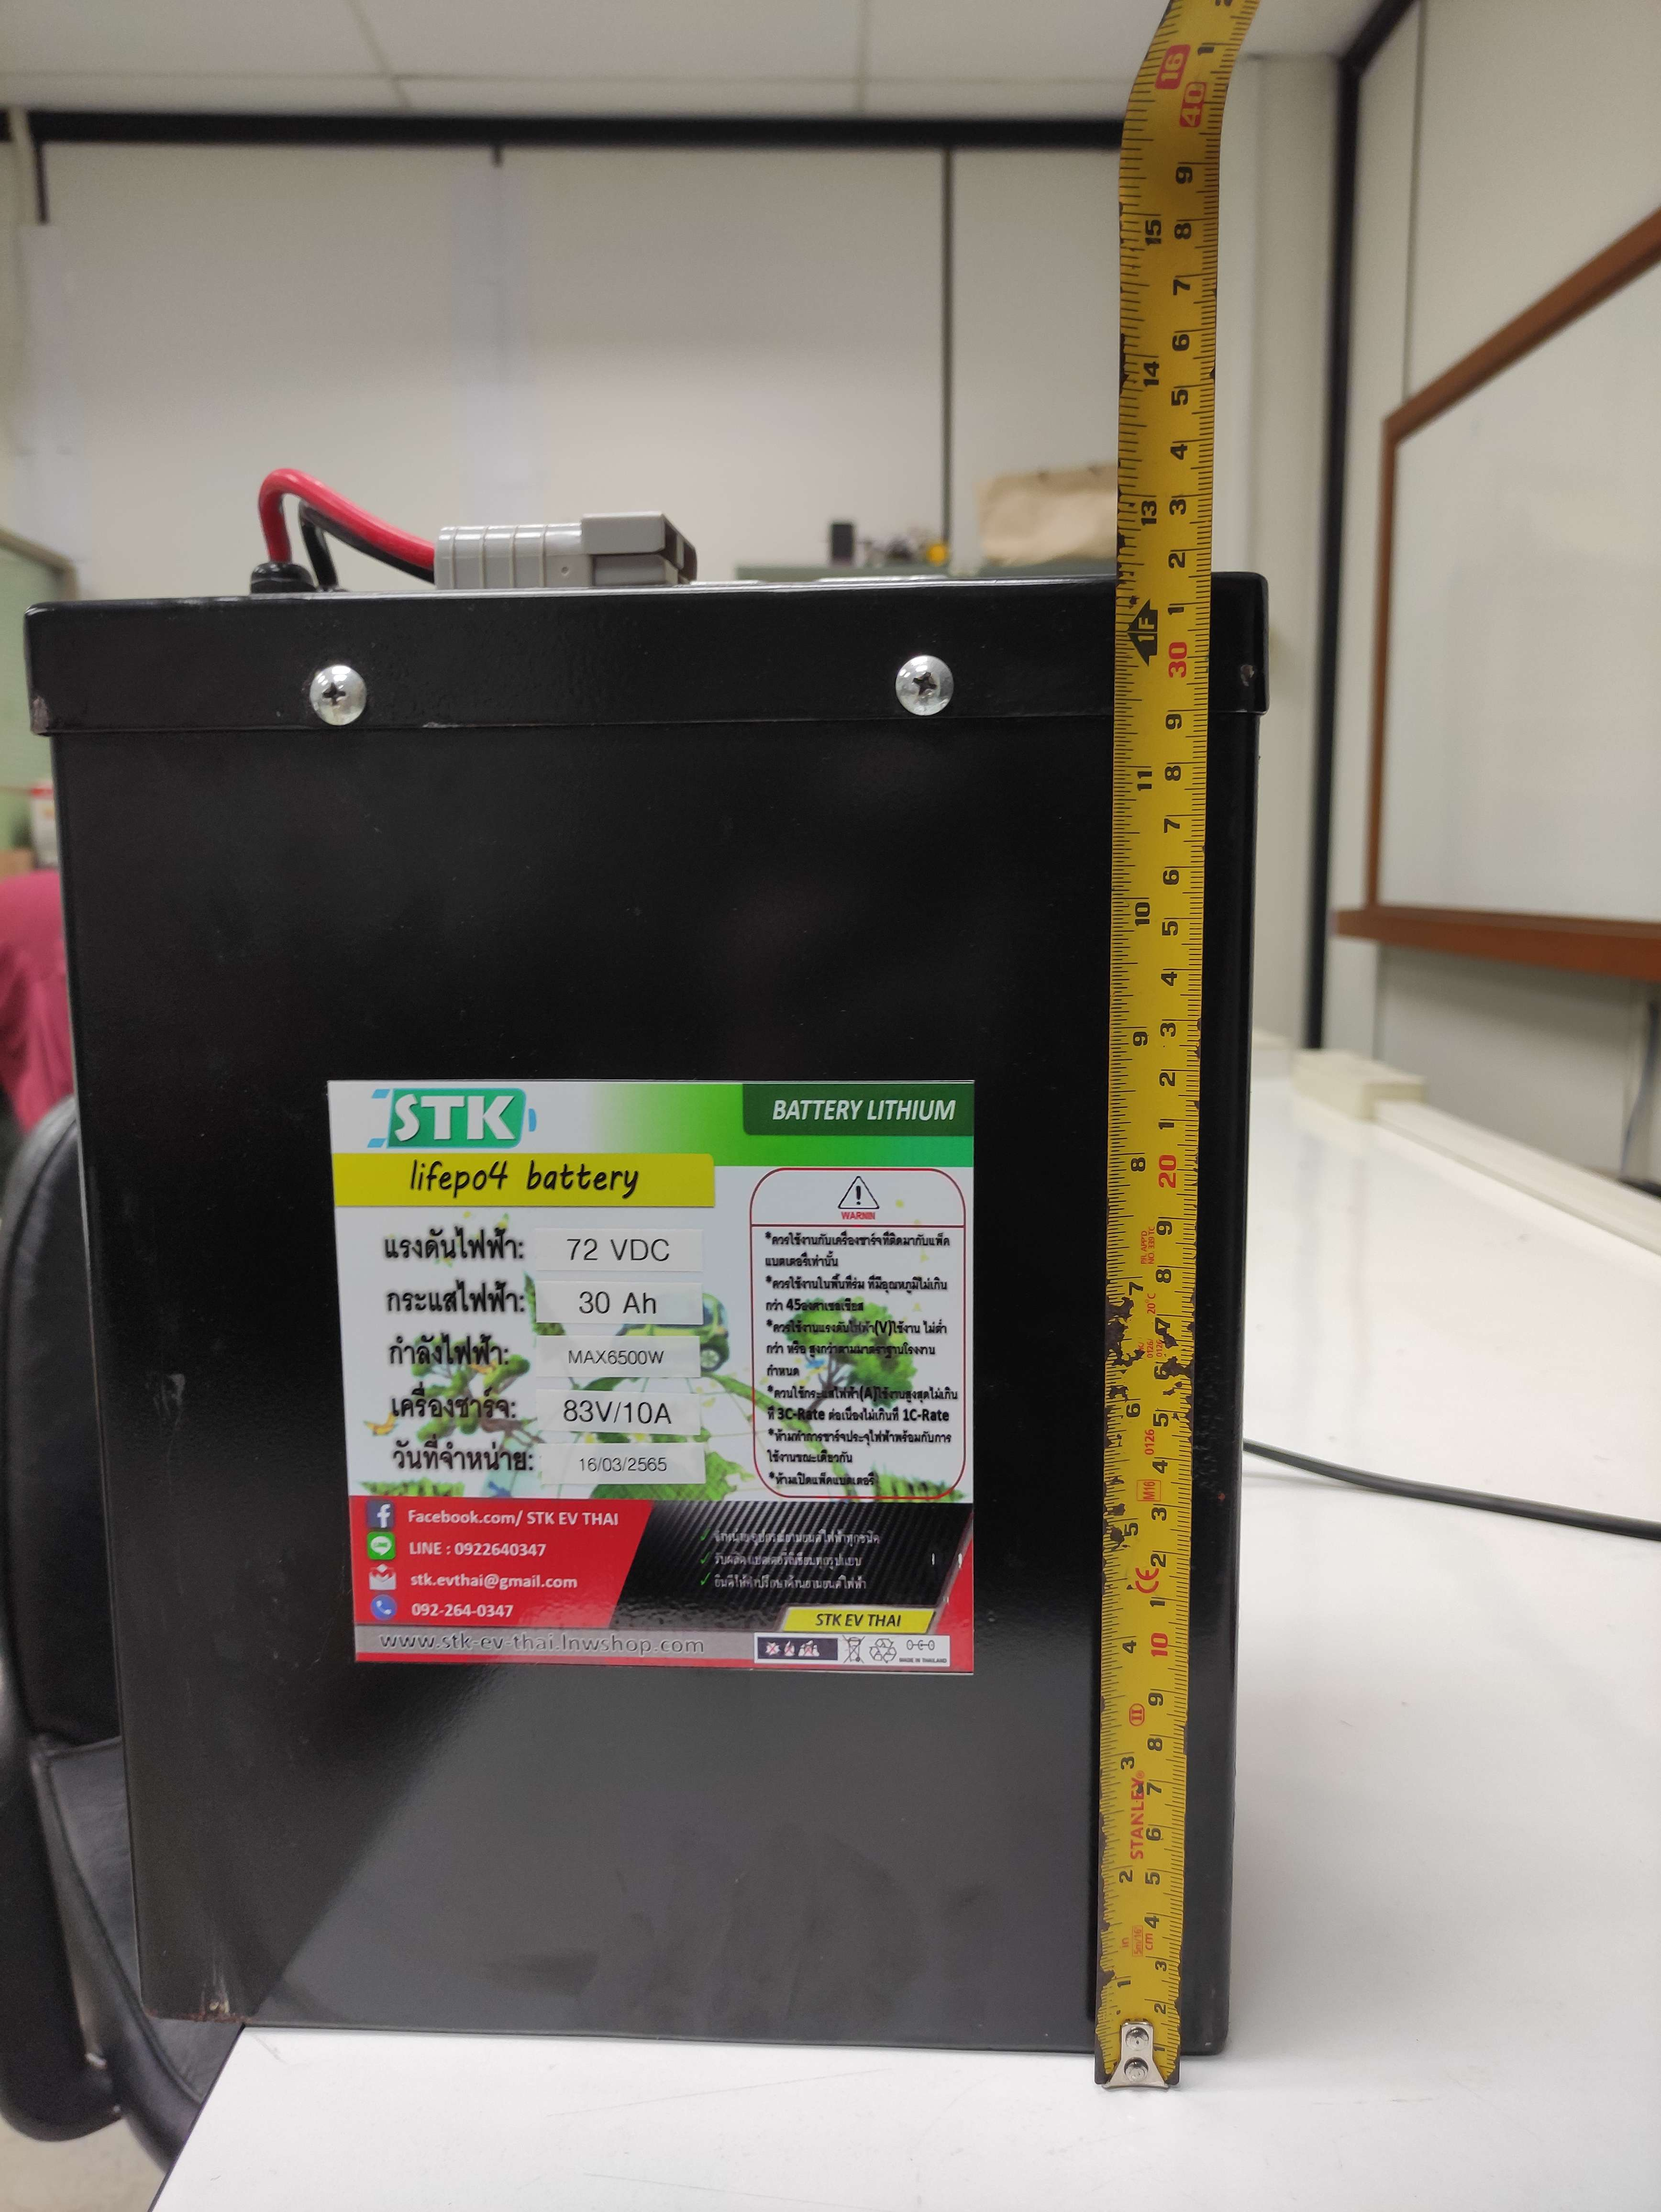
\includegraphics[width=0.5\linewidth]{Chapters/img/Battery_72V_30AH}
		\centering
		\captionsetup{justification=centering,margin=2cm}
		\caption{แบตเตอรี่สำหรับทำการทดสอบ}
	\end{figure}
\end{center}
%========================================================================================================
โดยใช้งานเครื่องทดสอบแบตเตอรี่ในการทดสอบแบตเตอรี่ในแต่ละหัวข้อมีดังนี้
%========================================================================================================
%\subsection{การใช้เครื่องทดสอบแบตเตอรี่ Chroma Model 17020 \\ ในการทดสอบการป้องกันการลัดวงจรภายนอกของแบตเตอรี่}
%สำหรับหัวข้อการทดสอบการป้องกันการลัดวงจรภายนอกของแบตเตอรี่
%========================================================================================================
\subsection{การใช้เครื่องทดสอบแบตเตอรี่ Chroma Model 17020 \\ ในการทดสอบการป้องกันการชาร์จเกินของแบตเตอรี่}
สำหรับหัวข้อการทดสอบการป้องกันการชาร์จเกินของแบตเตอรี่โดยใช้เครื่องทดสอบแบตเตอรี่ Chroma Model 17020 ในการทดสอบพารามิเตอร์ต่างๆจะถูกตั้งค่าให้เหมาะสมสำหรับการทดสอบตามมาตรฐาน UN ECE Regulation 136 โดยให้เครื่องทดสอบแบตเตอรี่ทำการชาร์จแบตเตอรี่ด้วยโหมดแรงดันและกระแสคงที่(CC-CV)ที่แรงดัน 84V และอัตรากระแส 1/3C หรือสำหรับแบตเตอรี่ที่ใช้สำหรับการทดสอบนี้คือ 10A
และจะชาร์จจนกว่าระบบป้องกันการชาร์จเกินของแบตเตอรี่ในที่นี้คือระการจัดการแบตเตอรี่(BMS)จะทำการขัดจังหวะการชาร์จเพื่อป้องกันการดิสชาร์จเกินของแบตเตอรี่โดยขณะที่ระบบป้องกันของเครื่องทดสอบแบตเตอรี่จะป้องกันในเรื่องของ
ป้องกันกระแสชาร์จเกิน12A ป้องกันแรงดันสูงเกิน2เท่าของแรงดันพิกัดแบตเตอรี่ที่ใช้ทำการทดสอบในที่นี้คือ 170V และป้องกันแรงดันต่ำเกิน 50\% SOC หรือในที่นี้คือ 36V โดยการตั้งค่าต่างๆจะเป็นไปดังรูป
\begin{center}
	\begin{figure}[H]
		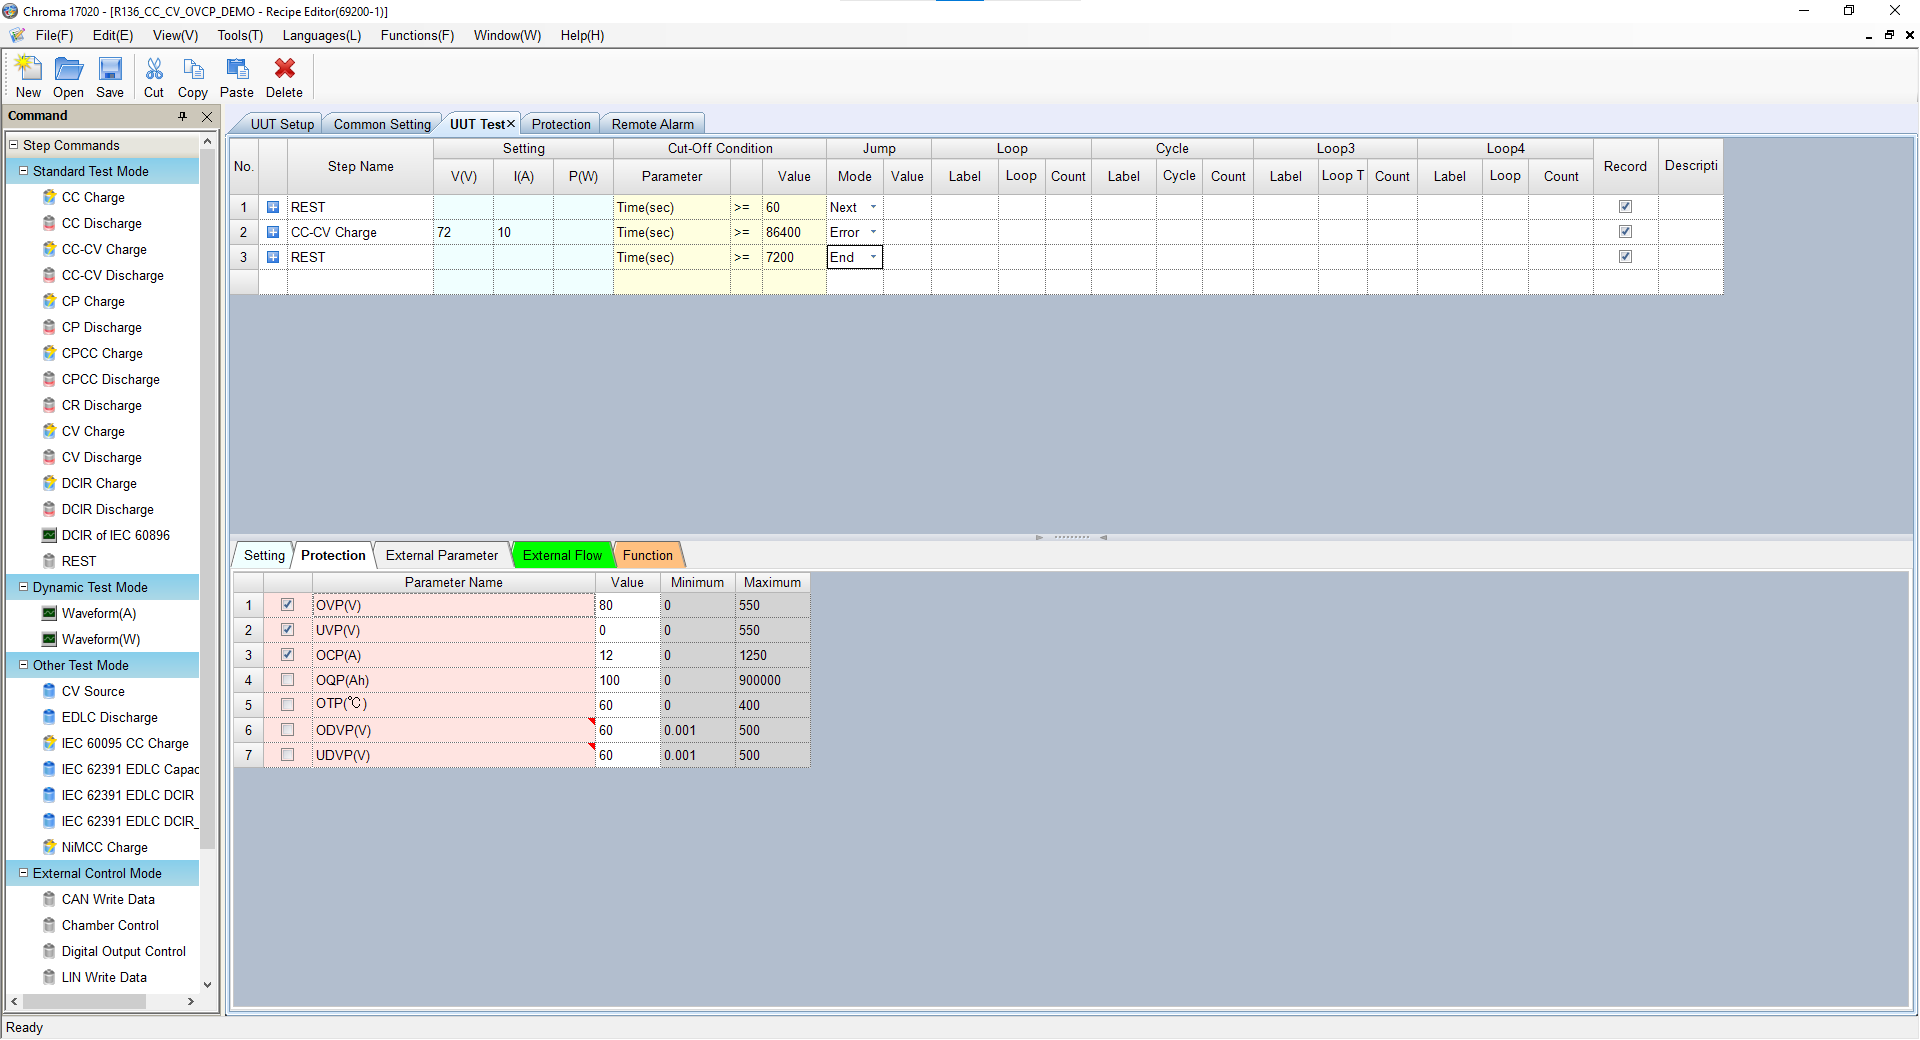
\includegraphics[width=1\linewidth]{Chapters/img/R136_DEMO/UUT_TEST_OVCP.png}
		\centering
		\captionsetup{justification=centering,margin=2cm}
		\caption{การตั้งค่าสำหรับการทดสอบการป้องกันการชาร์จเกินของแบตเตอรี่}
	\end{figure}
\end{center}
%========================================================================================================
\subsection{การใช้เครื่องทดสอบแบตเตอรี่ Chroma Model 17020 \\ ในการทดสอบการป้องกันการดิสชาร์จเกินของแบตเตอรี่}
ในการทดสอบการป้องกันการดิสชาร์จเกินของแบตเตอรี่โดยใช้เครื่องทดสอบแบตเตอรี่ Chroma Model 17020 ในการทดสอบพารามิเตอร์ต่างๆจะถูกตั้งค่าให้เหมาะสมสำหรับการทดสอบตามมาตรฐาน UN ECE Regulation 136 โดยให้เครื่องทดสอบแบตเตอรี่ทำการดิสชาร์จแบตเตอรี่ด้วยโหมดกระแสคงที่(CC)ด้วยอัตรา 1/3C หรือสำหรับแบตเตอรี่ที่จะทำการทดสอบก็คือกระแสขนาด 10A โดยจะดิสชาร์จต่อเนื่องจนกว่า
ระบบป้องกันการดิสชาร์จเกินของแบตเตอรี่ในที่นี้คือระการจัดการแบตเตอรี่(BMS)จะทำการขัดจังหวะการดิสชาร์จเพื่อป้องกันการดิสชาร์จเกินของแบตเตอรี่โดยขณะที่ระบบป้องกันของเครื่องทดสอบแบตเตอรี่จะป้องกันในเรื่องของ
ป้องกันกระแสดิสชาร์จเกิน12A ป้องกันแรงดันต่ำเกิน 24\% SOC หรือในที่นี้คือ 17.28V และป้องกันแรงดันเกิน 85V โดยการตั้งค่าต่างๆจะเป็นไปดังรูป
\begin{center}
	\begin{figure}[H]
		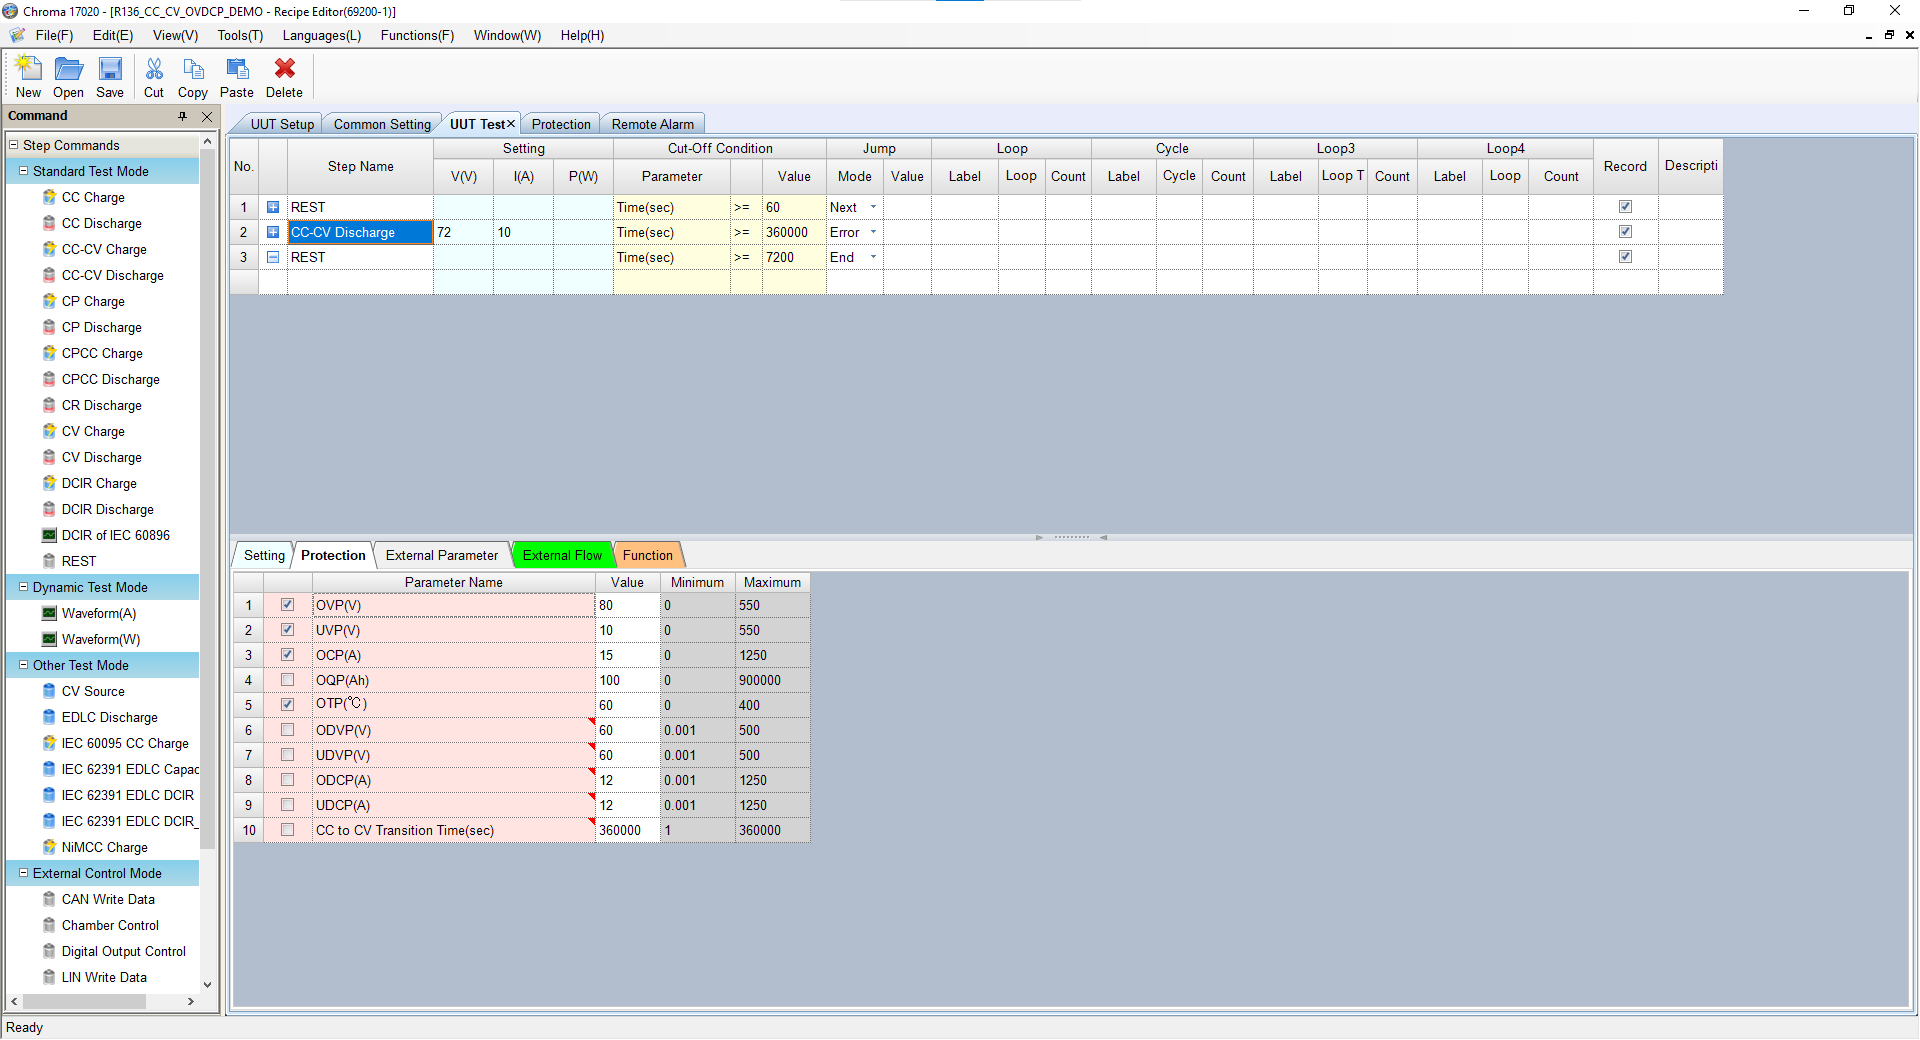
\includegraphics[width=1\linewidth]{Chapters/img/R136_DEMO/UUT_TEST_OVDCP.png}
		\centering
		\captionsetup{justification=centering,margin=2cm}
		\caption{การตั้งค่าสำหรับการทดสอบการป้องกันการดิสชาร์จเกินของแบตเตอรี่}
	\end{figure}
\end{center}

















%\part{short title} % optional
\chapter{Results and discussion}
\nopagebreak
\chapter{บทสรุปและข้อเสนอแนะ}
\section{สรุปผลการทดสอบแบตเตอรี่}
จากการทดสอบแบตเตอรี่ในหัวข้อการทดสอบการป้องกันการชาร์จเกินจากมาตรฐาน UN ECE R136 จะเห็นได้ว่าสำหรับแบตเตอรี่สำหรับรถจักยานยนต์ไฟฟ้า 72V30Ah โมดูลนี้ผ่านการทดสอบไปได้
โดยที่ไม่เกิดความเสียหายกับแบตเตอรี่โมดูลนี้เนื่องจากแบตเตอรี่โมดูลนี้มีระบบการจัดการแบตเตอรี่(BMS)ที่ทำหน้าที่ป้องกันแบตเตอรี่ไม่ให้มีการชาร์จเกินแรงดันสูงสุดของแบตเตอรี่และขัดจังหวะการชาร์จระหว่างการทดสอบ
จึงทำให้ผ่านการทดสอบด้วยดีสำหรับแบตเตอรี่สำหรับรถสามล้อไฟฟ้า 72V60Ah จากการทดสอบการป้องกันการชาร์จเกินนี้เนื่องจากไม่ได้ทำการทดสอบที่ถูกต้องซึ่งเกิดจากการที่ทำการชาร์จโดยไม่ได้ชาร์จ
ตามที่ผู้ผลิตกำหนดโดยใช้ช่องทางการชาร์จเดียวกับช่องทางการดิสชาร์จซึ่งทางผู้ผลิตได้กำหนดให้ทำการชาร์จตรงช่องทางการชาร์จเช่นเดียวกันกับการดิสชาร์จผู้ผลิตกำหนดให้ดิสชาร์จตรงช่องทางการดิสชาร์จโดยผลการทดลองพบว่าข้อมูล
ไม่เพียงพอต่อการสรุปว่าผ่านการทดสอบหรือไม่เนื่องจากเหตุผลข้างต้นสำหรับแบตเตอรี่ 72V72Ah หลังจากการทดสอบการป้องกันการชาร์จเกินพบว่าผ่านการทดสอบเช่นเดียวกับแบตเตอรี่สำหรับรถจักรยานยนต์ไฟฟ้า
โดยที่มีระบบการจัดการแบตเตอรี่(BMS)ขัดจังหวะการทดสอบเพื่อป้องกันแรงดันของแบตเตอรี่เกินกว่าที่กำหนดและการทำงานของระบบการจัดการแบตเตอรี่ของโมดูลแบตเตอรี่ 72V30Ah พบว่าทำการขัดจังหวะการชาร์จที่แรงดัน
ตามที่ได้ตั้งค่าไว้โดยที่ขัดจังหวะที่แรงดัน 83.9V ซึ่งจากการที่ได้ตั้งค่าไว้ควรจะขัดจังหวะที่ 84V และสำหรับระบบการจัดการแบตเตอรี่สำหรับโมดูลแบตเตอรี่ 72V72Ah พบว่าทำการขัดจังหวะการชาร์จที่แรงดัน
77.6V ซึ่งจากตารางคุณสมบัติของระบบการจัดการแบตเตอรี่นี้ควรจะขัดจังหวะการชาร์จที่ $78.1\pm 1.1V$ 
\newline
\hspace*{2cm}
และจากการทดสอบแบตเตอรี่ในหัวข้อการทดสอบการป้องกันการดิสชาร์จเกินจากมาตรฐาน UN ECE R136 จะเห็นได้ว่าสำหรับแบตเตอรี่สำหรับรถจักยานยนต์ไฟฟ้า 72V30Ah โมดูลนี้ผ่านการทดสอบไปได้
โดยที่ไม่เกิดความเสียหายกับแบตเตอรี่โมดูลนี้เนื่องจากแบตเตอรี่โมดูลนี้มีระบบการจัดการแบตเตอรี่(BMS)ป้องกันไม่ให้แบตเตอรี่แรงดันต่ำเกินกว่าที่กำหนดซึ่งการทดสอบถูกขัดจังหวะโดยระบบการจัดการแบตเตอรี่สำหรับ
แบตเตอรี่สำหรับรถสามล้อไฟฟ้า 72V60Ah เช่นเดียวกันกับแบตเตอรี่สำหรับรถจักรยานยนต์ไฟฟ้าแบตเตอรี่โมดูลนี้ผ่านการทดสอบโดยมีระบบการจัดการแบตเตอรี่ขัดจังหวะการทดสอบและสุดท้ายสำหรับแบตเตอรี่ 72V72Ah
เช่นเดียวกันกับการทดสอบแบตเตอรี่โมดูลที่ผ่านแบตเตอรี่โมดูลนี้ผ่านการทดสอบโดยมีระบบการจัดการแบตเตอรี่ขัดจังหวะการทดสอบทำให้ผ่านการทดสอบโดยไม่เกิดความเสียหายกับแบตเตอรี่เช่นกัน 
โดยการขัดจังหวะการดิสชาร์จของระบบการจัดการแบตเตอรี่ของโมดูลแบตเตอรี่ 72V30Ah พบว่าขัดจังหวะการดิสชาร์จที่ 61.582V ซึ่งจากการตั้งค่าควรจะขัดจังหวะที่ 58V จากการขัดจังหวะของระบบการจัดการแบตเตอรี่ของโมดูลแบตเตอรี่ 72V60Ah ขัดจังหวะการดิสชาร์จที่แรงดัน 57.3678V โดยจากการที่ไม่ทราบคุณสมบัติของโมดูลแบตเตอรี่และระบบการจัดการแบตเตอรี่นี้อย่างละเอียดและชัดเจนจึงไม่สามารถทำการสรุปได้และจากการขัดจังหวะของระบบการจัดกรแบตเตอรี่ของโมดูลแบตเตอรี่ 72V72Ah พบว่าขัดจังหวะการดิสชาร์จที่ 62.3V ซึ่งจากตารางคุณสมัติแล้วควรจะขัดจังหวะการดิสชาร์จที่ $50.6\pm 1.1V$ โดยจะเห็นได้ว่าทั้งระบบการจัดการแบตเตอรี่ของโมดูลแบตเตอรี่ 72V30Ah และ 72V72Ah ทำการขัดจังหวะการดิสชาร์จก่อนถึงแรงดันที่ควรจะขัดจังหวะไว้ซึ่งอาจจะส่งผลให้ช่วงแรงดันหรือช่วงความจุที่ใช้โมดูลแบตเตอรี่นั้นลดลงไปกว่าที่ควร
%และจะเห็นได้ว่า
%แบตเตอรี่ที่ผ่านการทดสอบทั้งการป้องกันการชาร์จเกินและการป้องกันการดิสชาร์จเกินผ่านการทดสอบเนื่องจากมีระบบป้องกันไม่ให้โมดูลแบตเตอรี่มีแรงดันต่ำเกินและสูงเกินในกรณีที่ไม่มีระบบป้องกันนี้จึงไม่สามารถทราบได้ว่าผลการทดสอบ
%จะเป็นอย่างไร
\newline
\hspace*{2cm}
จากการทดสอบการวัดความต้านทานภายในในการทดสอบสามารถทดสอบจะทดสอบเฉพาะโมดูลแบตเตอรี่ 72V72Ah เนื่องจากทราบคุณสมบัติชัดเจนทำให้มีความปลอดภัยต่อการทดสอบซึ่งจากการทดสอบพบว่าขณะที่แบตเตอรี่
แรงดันขณะดิสชาร์จที่อัตรากระแส 0.2C โมดูลแบตเตอรี่นี้มีแรงดัน 72V และขณะที่ดิสชาร์จที่อัตรากระแส 1C แรงดันลดลงอย่างเรวดเร็วซึ่งอยู่ที่ 70.4V จากข้อมูลนี้จึงทำให้ได้ค่าความต้านทานภายในอยู่ที่
$26.8 m\Omega $ ทั้งนี้ความต้านทานภายในเปลี่ยนแปลงไปตามแรงดัน ณ ขณะที่ทดสอบซึ่งการทดสอบนี้ทดสอบที่แรงดันค่าหนึ่งเท่านั้นนั่นก็คือ 72V
\newline
\hspace*{2cm}
จากการทดสอบเพื่อหาระยะเวลาพักแบตเตอรี่ที่แบตเตอรี่นั้นจะไม่เกิดการเปลี่ยนแปลงซึ่งจะเห็นได้ว่าแรงดันเริ่มที่จะหยุดเปลี่ยนแปลงเมื่อทำการพักมาแล้วเป็นระยะเวลาประมาณ 30 นาทีซึ่งสรุปได้ว่าระยะเวลานี้เป็นระยะเวลาพักที่เหมาะสมก่อนที่จะทำการทดสอบอย่างอื่นต่อไปเพื่อความแม่นยำในการทดสอบต่างๆและสุดท้ายจากการทดสอบอัตรากระแสมีผลต่ออัตรากระแสนี้
จะเห็นได้ว่าเมื่ออัตรากระแสเปลี่ยนแปลงไปทำให้แรงดันต่อช่วงความจุนั้นเปลี่ยนแปลงซึ่งถ้าหากใช้อัตรากระแสที่มากจะทำให้แรงดันมีการเปลี่ยนแปลงที่รวดเร็วกว่าการใช้อัตรากระแสที่น้อยกว่า
%================================================================================
\section{แนวทางการแก้ปัญหา}
เนื่องจากโมดูลแบตเตอรี่สำหรับรถสามล้อไฟฟ้านั้นไม่ทราบคุณสมบัติโดยละเอียดซึ่งทราบเพียงพิกัดและชนิดของแบตเตอรี่เพียงเท่านั้นและจากการที่ช่องทางการชาร์จของโมดูลแบตเตอรี่นี้มีระบบการจัดการหรือระบบป้องกันที่
ทางผู้ผลิตได้ออกแบบไว้ซึ่งสามารถใช้ได้เฉพาะเครื่องชาร์จที่ผู้ผลิตได้กำหนดเอาไว้ซึ่งทางคณะผู้จัดทำไม่ทราบถึงการทำงานของระบบป้องกันหรือระบบการจัดการดังกล่าวทำให้ไม่สามารถทดสอบการชาร์จได้อย่างถูกต้องได้
เช่นเดียวกับโมดูลแบตเตอรี่สำหรับจักรยานยนต์ไฟฟ้า 72V30Ah ซึ่งไม่ทราบคุณลักษณะโดยละเอียดทำให้มีข้อจำกัดในการทดสอบโดยแนวทางการแก้ปัญหาทั้งสองนี้มีแนวทางการแก้ปัญหาคือ
\begin{itemize}
{\item ติดต่อสอบถามบริษัทผู้ผลิตหรือจำหน่ายสินค้าเพื่อขอรายละเอียดและคุณลักษณะโมดูลแบตเตอรี่เพิ่มเติม}
{\item ศึกษาเครื่องชาร์จโมดูลแบตเตอรี่สำหรับรถสามล้อไฟฟ้าและระบบป้องกันหรือระบบการจัดการของแบตเตอรี่โมดูลนี้เพิ่มเติม}
\end{itemize}
%================================================================================
\section{ข้อเสนอแนะ}
เนื่องจากอุปกรณ์ในการทดสอบนั้นไม่มีความพร้อมต่อการทดสอบมากเท่าที่ควรดังนั้นก่อนเริ่มการทดสอบควรศึกษาขั้นตอนการทดสอบอย่างละเอียดและตรวจสอบความพร้อมของอุปกรณ์และเครื่องมืออื่นๆที่ใช้สำหรับการทดสอบ
ก่อนเริ่มทำการทดสอบและควรกำหนดแผนการทดสอบก่อนการทดสอบอย่างชัดเจนทั้งนี้เพื่อความประหยัดเวลาและอาจจะลดขั้นตอนการทำงานบางอย่างที่ไม่จำเป็นได้




















































%\cite{Godsil-McKay} \cite{Runde} \cite{Yero&Team}

%	% BIBAUTO
\makeatletter
\ifdefined\@bibauto
\ifx\@bibauto\bibvancouver
% biblatex vancouver
\printbibliography[title=\bibname]
\else
% biblatex apa, biblatex chicago-notes (Turabian)
\printbibheading[title=\bibname]
\nobibintoc
\printbibliography[heading=subbibliography, keyword=bookth, title={หนังสือและบทความในหนังสือ}] % thai references
% use heading=none to remove heading of the list of references whose keyword is book and combine them with the list of references above.
\printbibliography[heading=none, keyword=book, title={หนังสือและบทความในหนังสือ}] % english references
\printbibliography[heading=subbibliography, keyword=proceeding, title={รายงานการประชุมทางวิชาการ}]
\printbibliography[heading=subbibliography, keyword=article, title={บทความวารสาร}]
\printbibliography[heading=subbibliography, keyword=thesis, title={วิทยานิพนธ์}]
\printbibliography[heading=subbibliography, keyword=report, title={รายงาน}]
\printbibliography[heading=subbibliography, keyword=manual, title={คู่มือ}]
\printbibliography[heading=subbibliography, keyword=booklet, title={จุลสาร}]
\printbibliography[heading=subbibliography, keyword=electronicmedia, title={สื่ออิเล็กทรอนิกส์}]
\printbibliography[heading=subbibliography, keyword=unpublished, title={เอกสารที่ไม่ตีพิมพ์}]
\printbibliography[heading=subbibliography, keyword=miscellaneous, title={เบ็ดเตล็ด}]
\fi\fi\makeatother





% BIBMANUAL
\makeatletter\ifdefined\@bibmanual
\begin{thebibliography}{}
	
	\item\textbf{หนังสือและบทความในหนังสือ} % remove when the vancouver style is active.
	\item % remove when the vancouver style is active.
	
	
	% set up references for turabian and apa styles
	\bibitem[First Author et al.(year)First Author, Second Author, and Third Author]{ID1}
	First Author, Second Author, and Third Author...
	
	
	\bibitem[First Author and Second Author(year)]{ID2}
	First Author, Second Author, and Third Author...
	
	
	\item % remove when the vancouver style is active.
	\item\textbf{บทความวารสาร} % remove when the vancouver style is active.
	\item % remove when the vancouver style is active.
	
	
	% example
	\bibitem[Jones et al.(1990)Jones, Baker, and Williams]{jon90}
	Jones, Baker, and Williams...
	
	\bibitem[James and Tony(1991)]{jam91}
	James and Tony...
	
	\bibitem[Jones et al.(1991)Jones, Robin, and Smith]{jon91}
	Jones, Robin, and Smith...
	
	
	\item % remove when the vancouver style is active.
	\item\textbf{วิทยานิพนธ์} % remove when the vancouver style is active.
	\item % remove when the vancouver style is active.
	
	
	\bibitem[Jones et al.(1990a)Jones, Baker, and Williams]{jon90a}
	Jones, Baker, and Williams...
	
	\bibitem[Jones et al.(1990b)Jones, Robin, and Smith]{jon90b}
	Jones, Robin, and Smith...
	
	\bibitem[Jones et al.(1990a)Jones, Baker, and Williams]{jon90aa}
	Jones, Baker, and Williams...
	
	\bibitem[Jones et al.(1990b)Jones, Robin, and Smith]{jon90ba}
	Jones, Robin, and Smith...
	
	\bibitem[Jones et al.(1990a)Jones, Baker, and Williams]{jon90ab}
	Jones, Baker, and Williams...
	
	\bibitem[Jones et al.(1990b)Jones, Robin, and Smith]{jon90bb}
	Jones, Robin, and Smith...
	
	
	
\end{thebibliography}
\fi\makeatother












	\bibliographystyle{IEEEtran}
	\bibliography{6_References}
	\appendix[nosub] % use \appendix if there are subappendices

%appendix text
%-------------------------------------------------------------------------------------------
\chapter{รูปอุปกรณ์เครื่องมือวัดและทดสอบ}
\begin{center}
 \begin{figure}[H]
		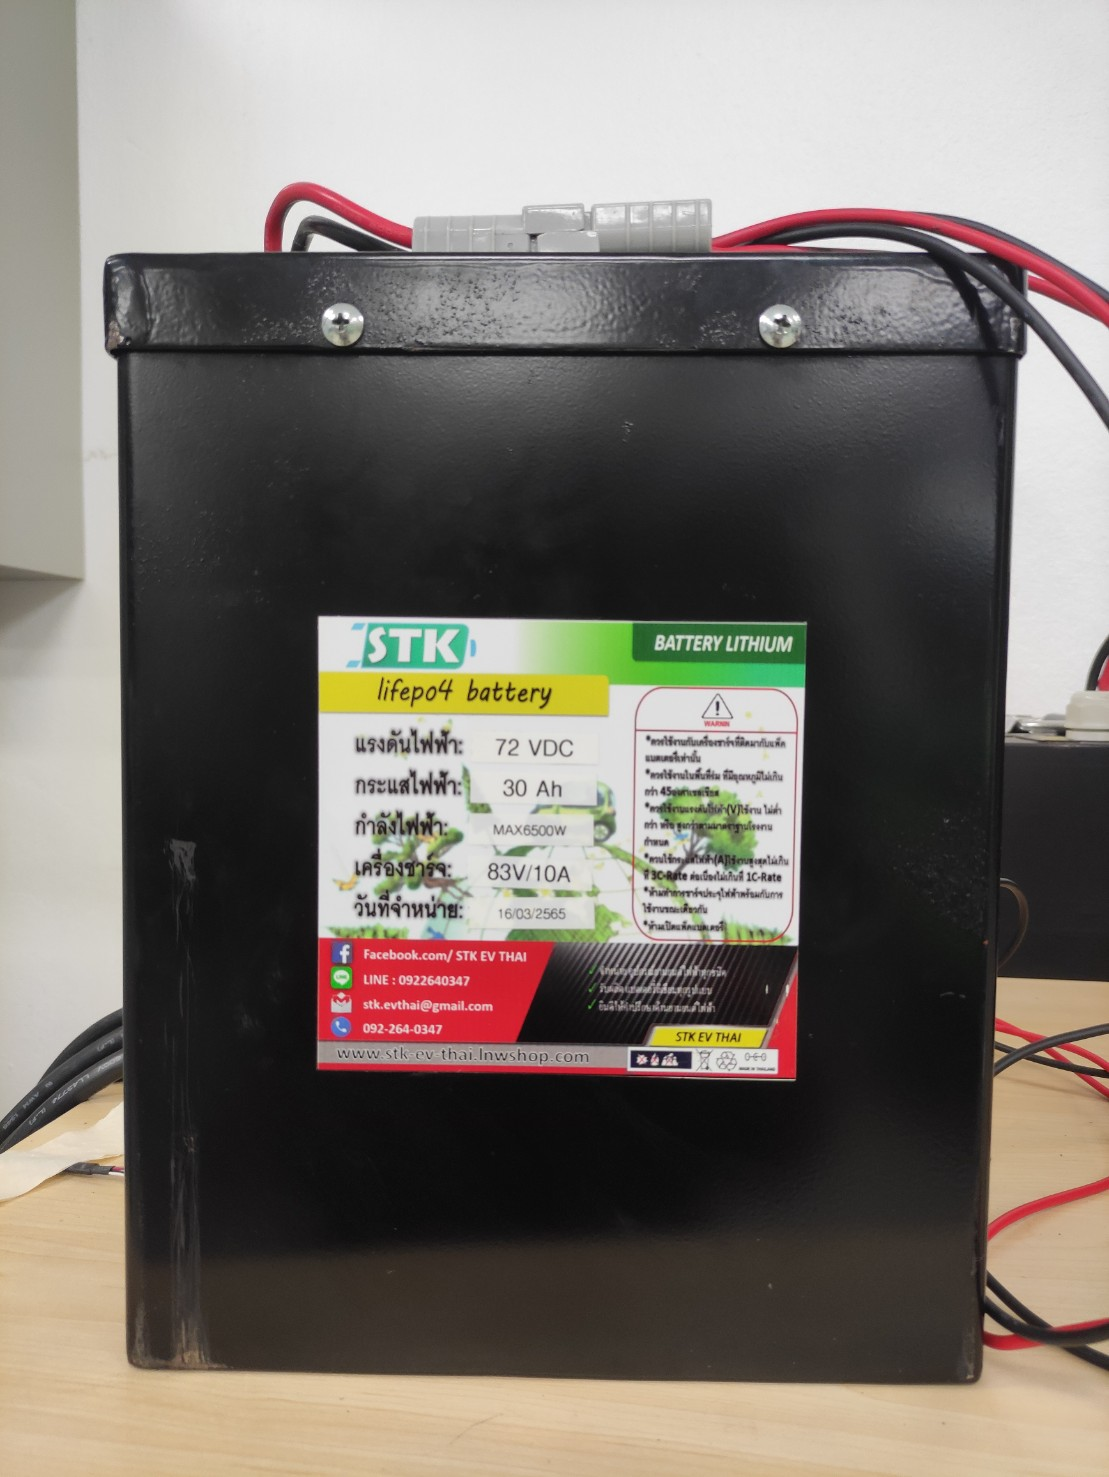
\includegraphics[width=0.5\linewidth]{Chapters/img/Battery_72V30Ah.jpg}
		\centering
		\captionsetup{justification=centering,margin=2cm}
		\caption{แบตเตอรี่สำหรับจักยานยนต์ไฟฟ้า 72V30Ah}
	\end{figure}
	\begin{figure}[H]
		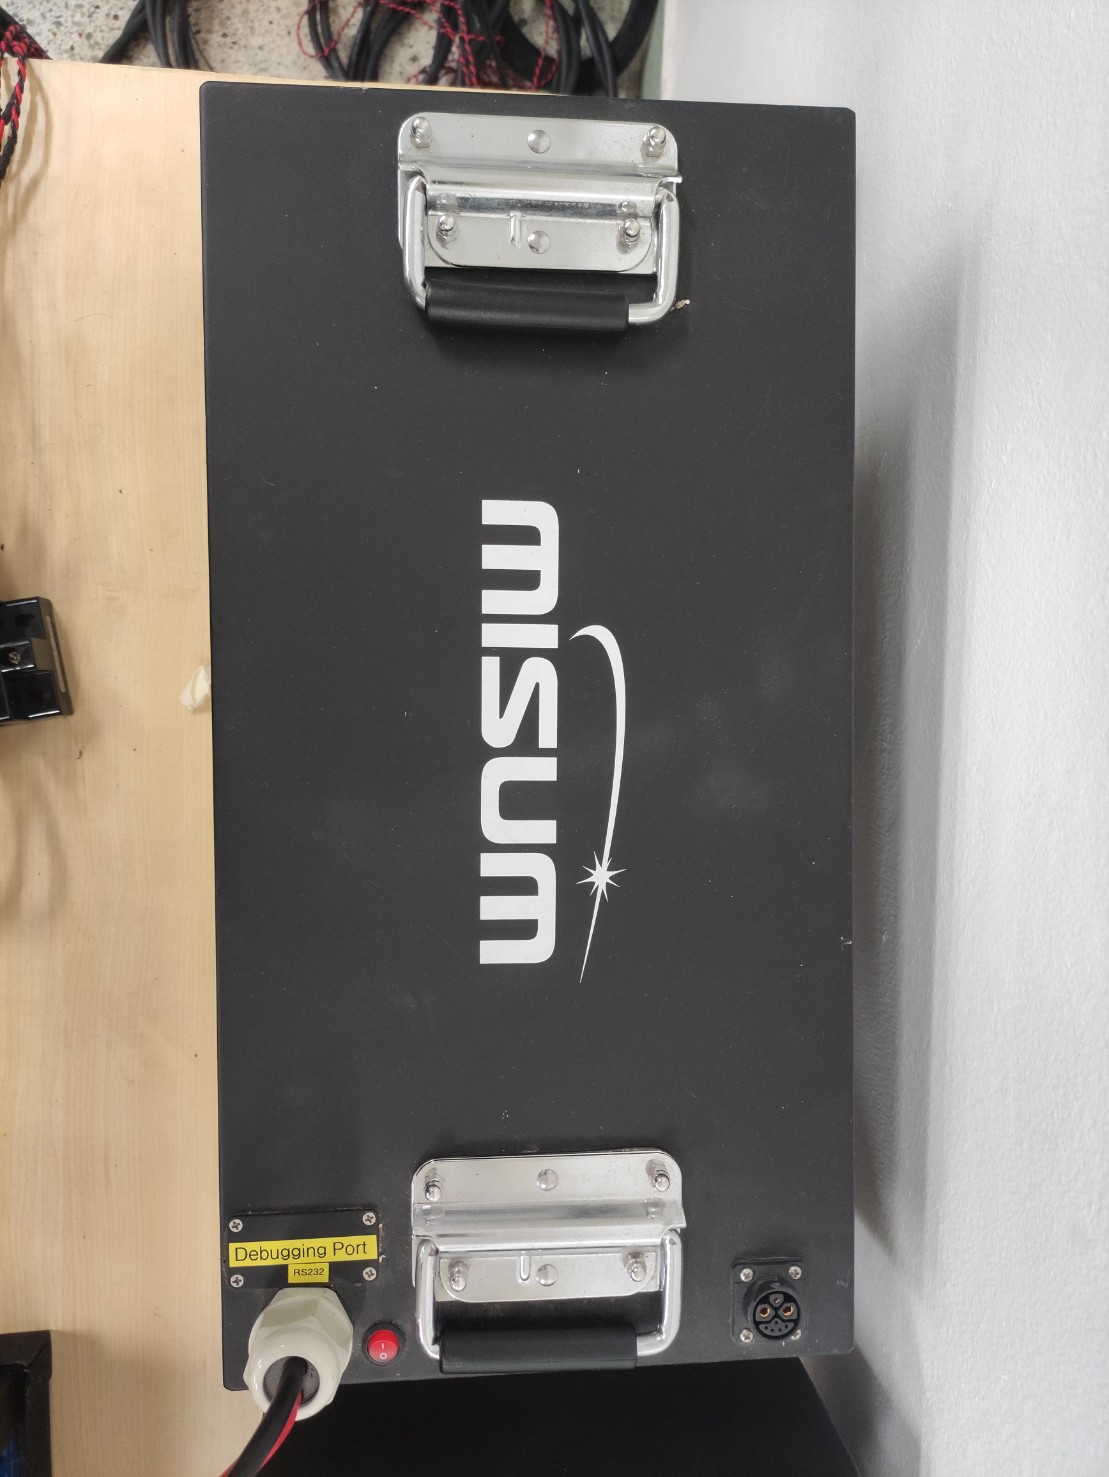
\includegraphics[width=0.5\linewidth]{Chapters/img/Battery_72V60Ah.jpg}
		\centering
		\captionsetup{justification=centering,margin=2cm}
		\caption{แบตเตอรี่สำหรับสามล้อไฟฟ้า 72V60Ah}
	\end{figure}
	\begin{figure}[H]
		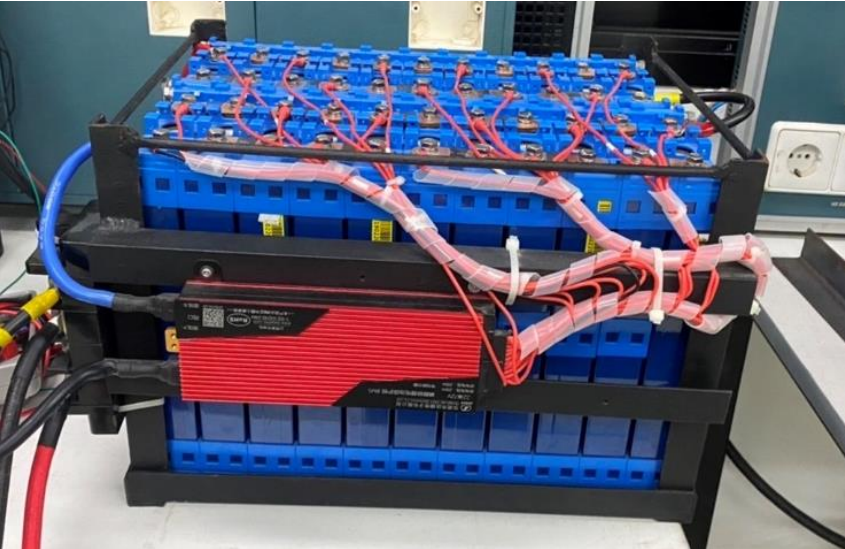
\includegraphics[width=0.5\linewidth]{Chapters/img/Battery_72V72Ah.jpg}
		\centering
		\captionsetup{justification=centering,margin=2cm}
		\caption{แบตเตอรี่ 72V72Ah}
	\end{figure}
	\begin{figure}[H]
		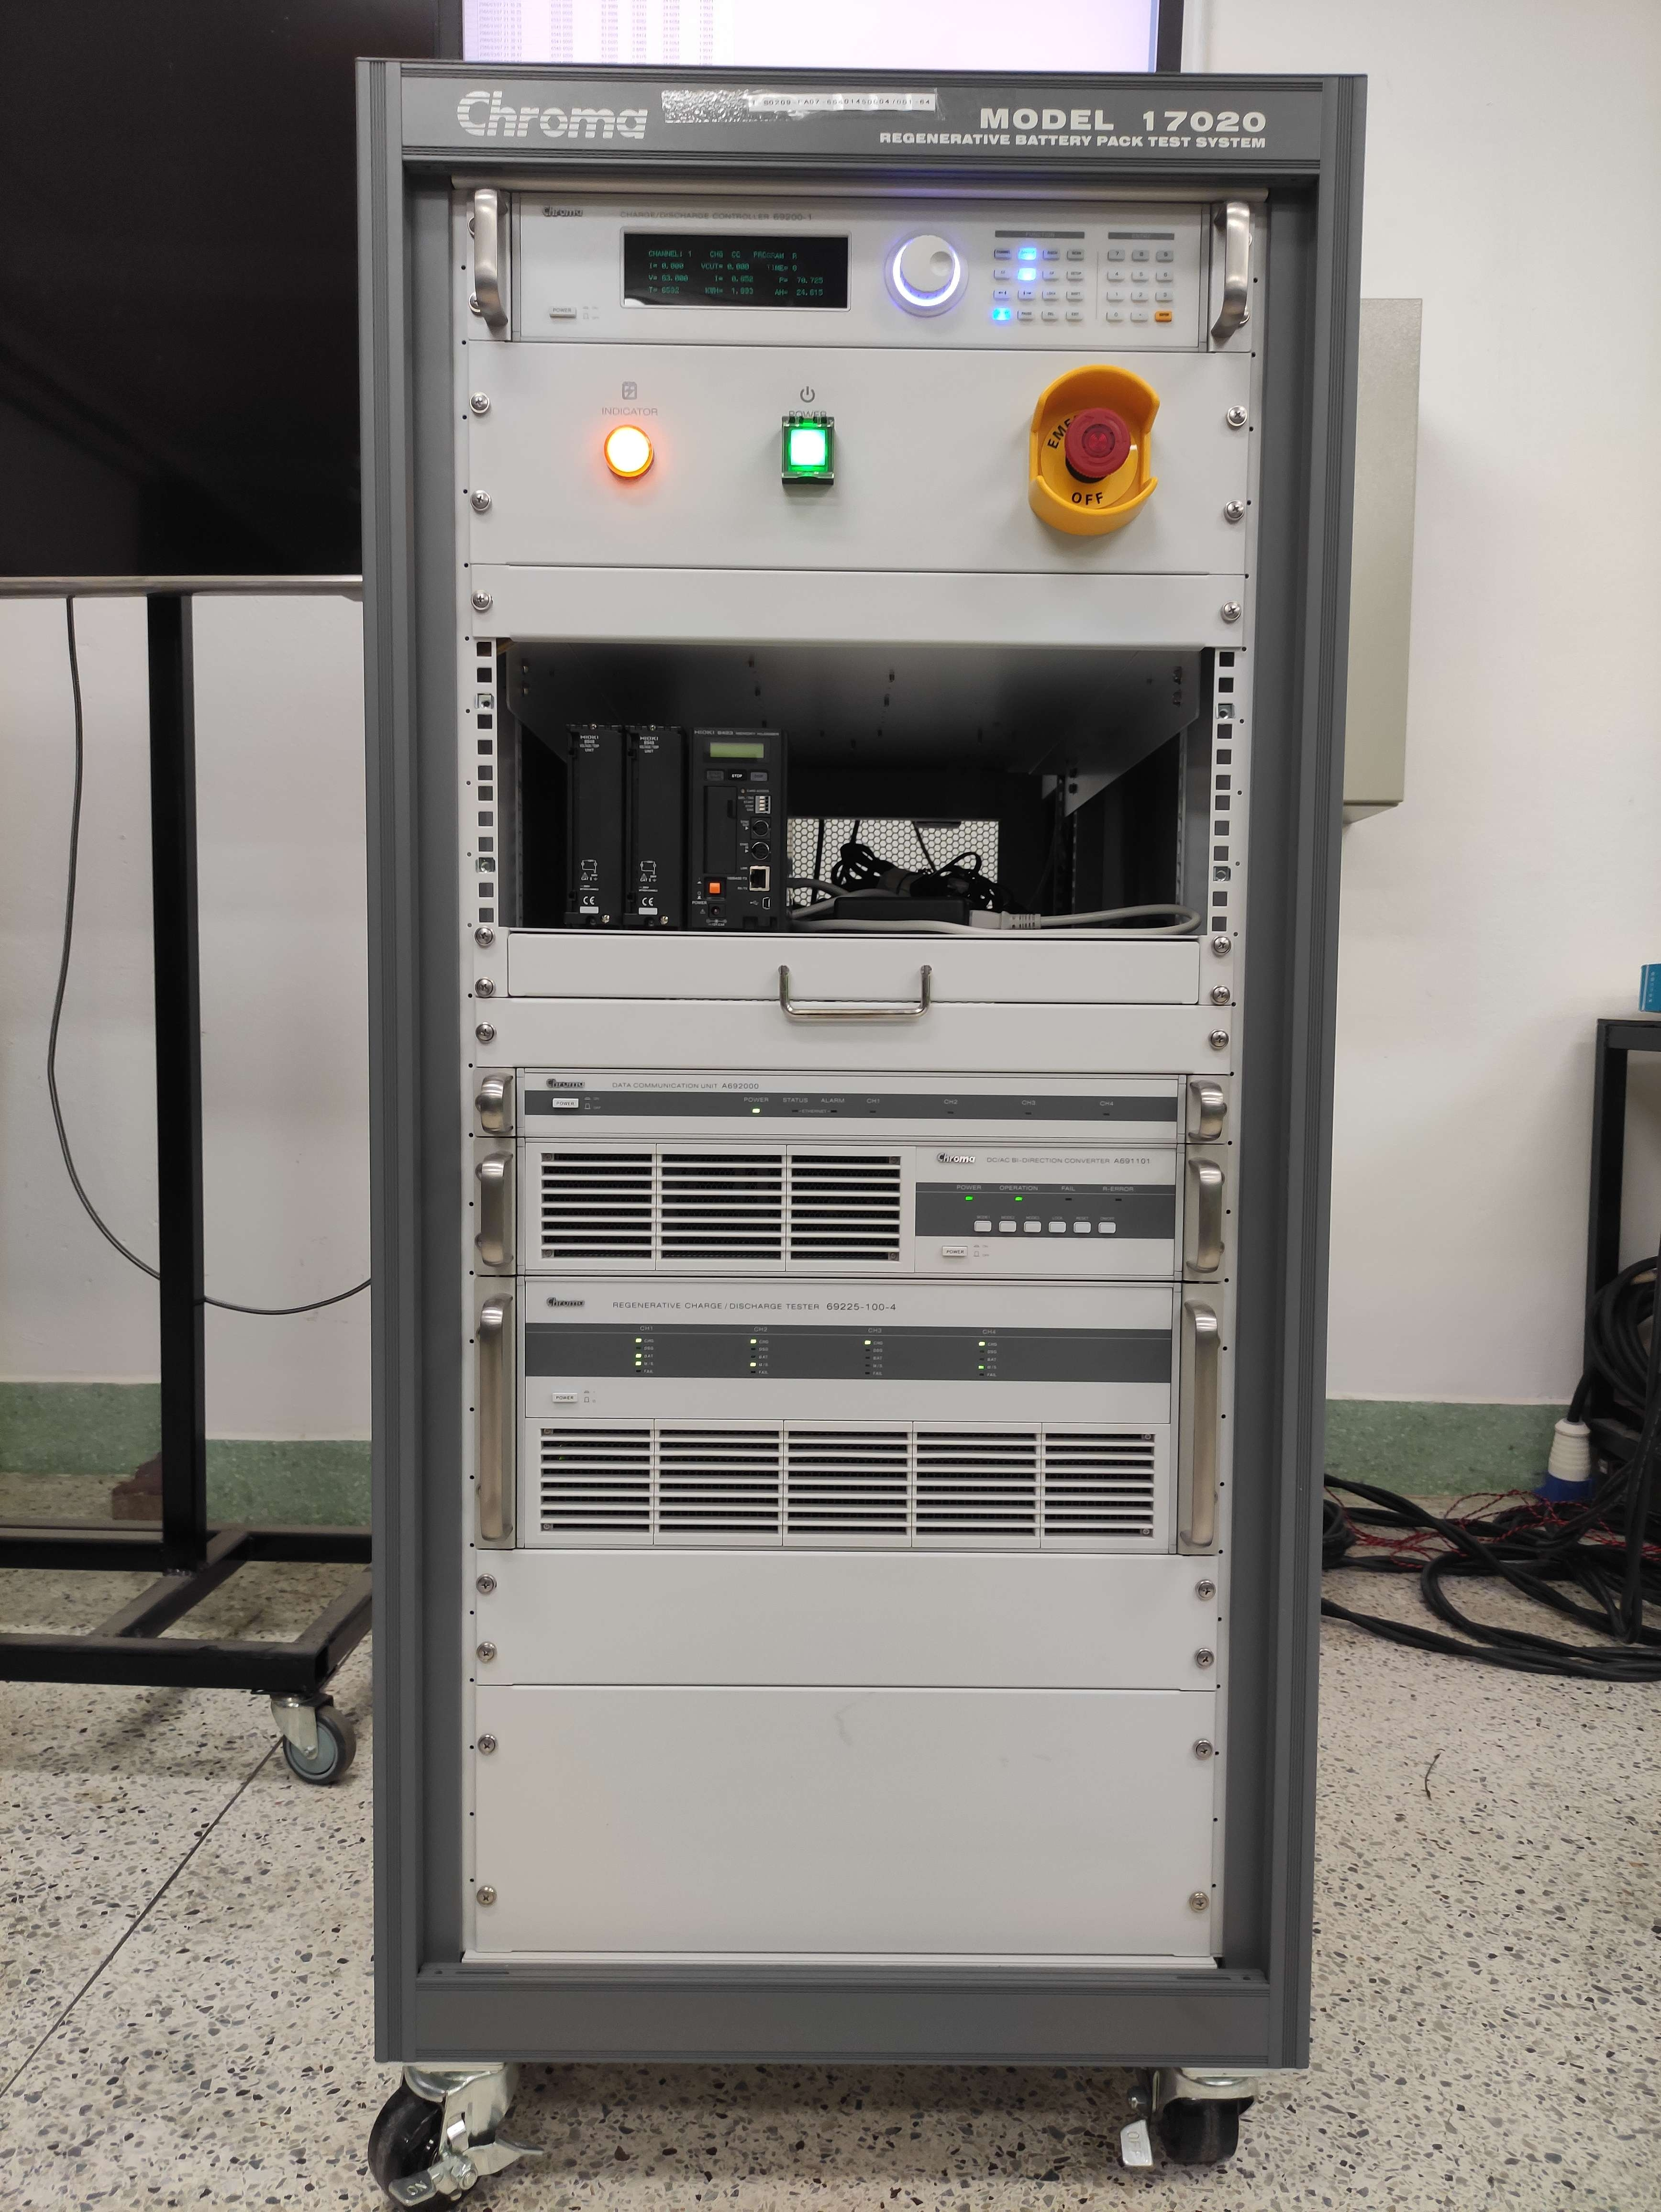
\includegraphics[width=0.5\linewidth]{Chapters/img/Chroma_17020.jpg}
		\centering
		\captionsetup{justification=centering,margin=2cm}
		\caption{เครื่องทดสอบแบตเตอรี่ Chroma model 17020}
		\label{fig:Chroma model 17020}
	\end{figure}
	\begin{figure}[H]
		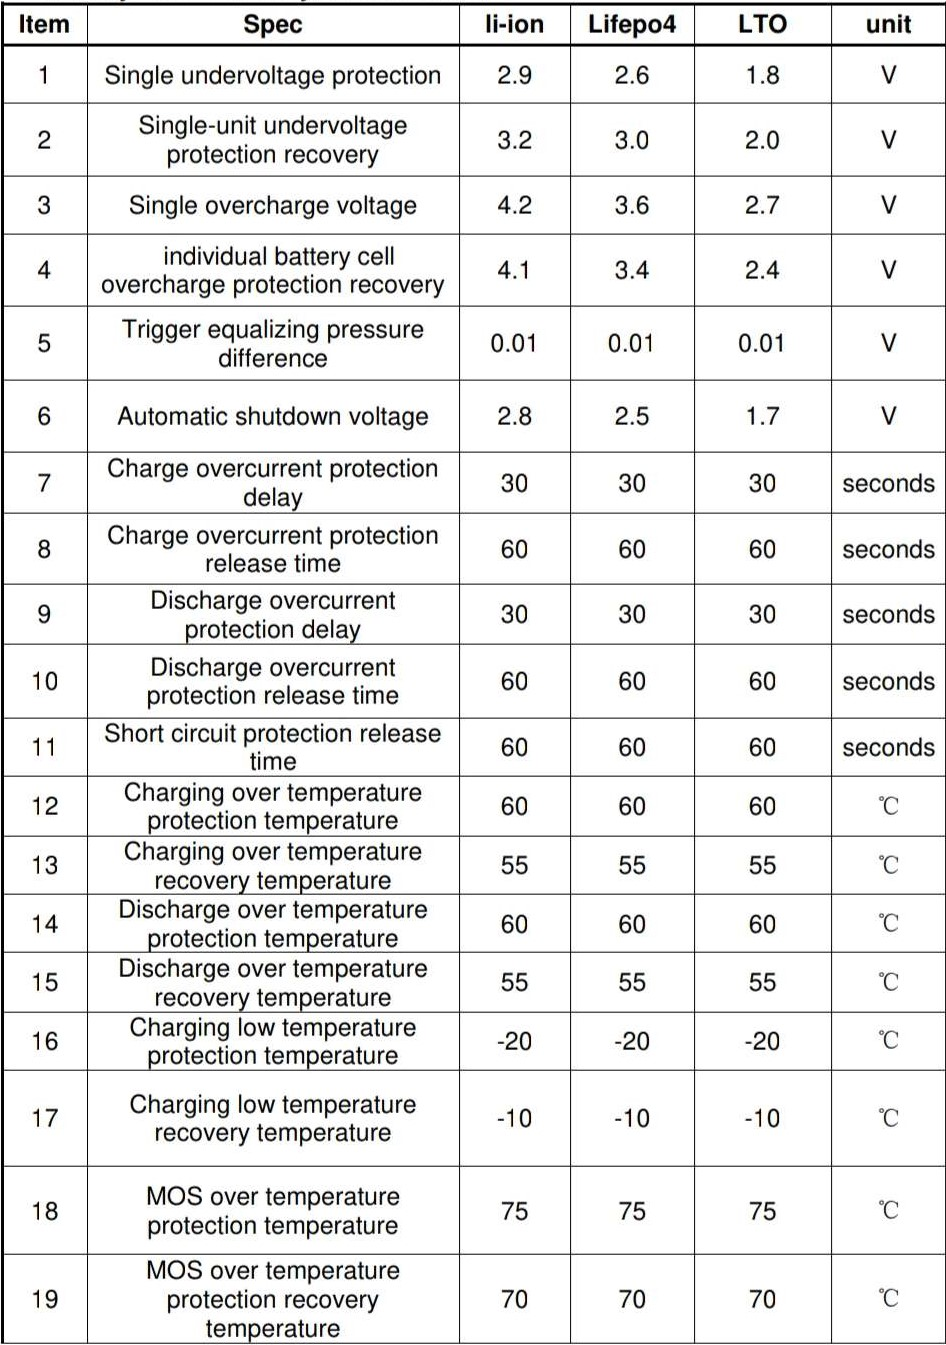
\includegraphics[width=0.5\linewidth]{Chapters/img/BMS_Setting.jpg}
		\centering
		\captionsetup{justification=centering,margin=2cm}
		\caption{ตารางการตั้งค่าตัวแปรของระบบการจัดการแบตเตอรี่ของโมดูลแบตเตอรี่ 72V30Ah}
		\label{fig:BMS_Setting}
	\end{figure}
	\begin{figure}[H]
		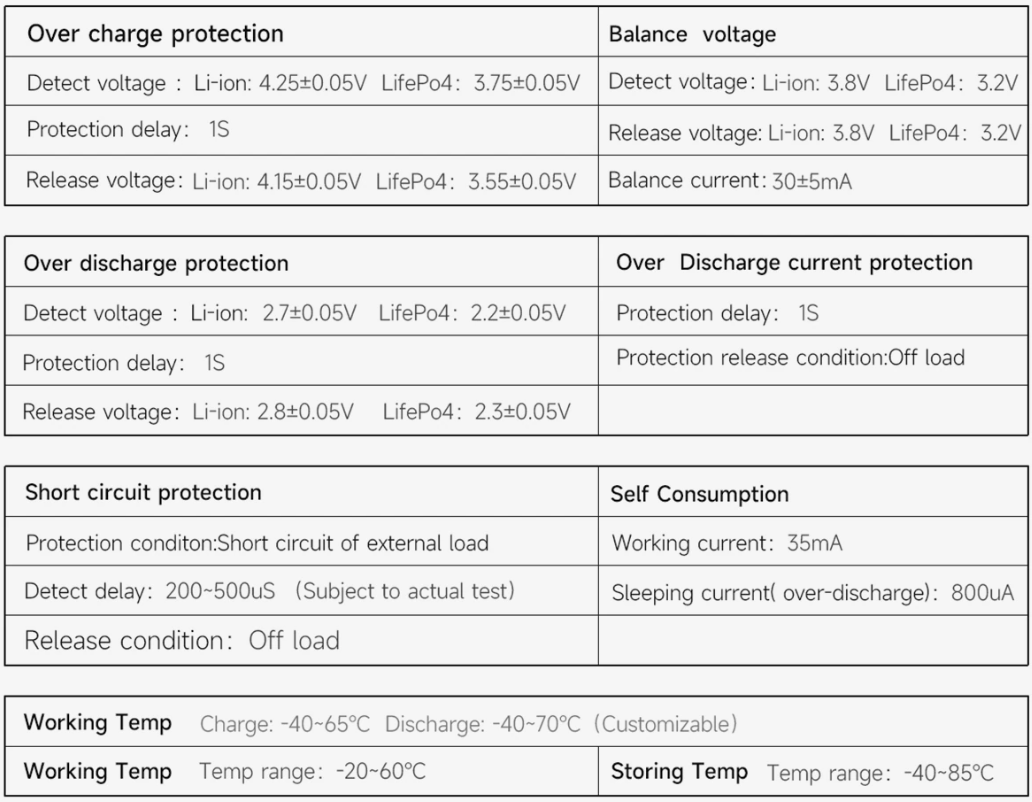
\includegraphics[width=1\linewidth]{Chapters/img/BMS_Setting2.PNG}
		\centering
		\captionsetup{justification=centering,margin=2cm}
		\caption{ตารางการตั้งค่าตัวแปรของระบบการจัดการแบตเตอรี่ของโมดูลแบตเตอรี่ 72V72Ah}
		\label{fig:BMS_Setting2}
	\end{figure}
\end{center}
%------------------------------------------------------------------------------------------
\chapter{คู่มือการใช้งานโปรแกรม Chroma 17020}
 เมื่อเปิดโปรแกรม Chroma 17020 จะพบกับหน้าเข้าสู่ระบบดังรูปที่\ref{fig:Loggin}
 \begin{center}
	\begin{figure}[H]
		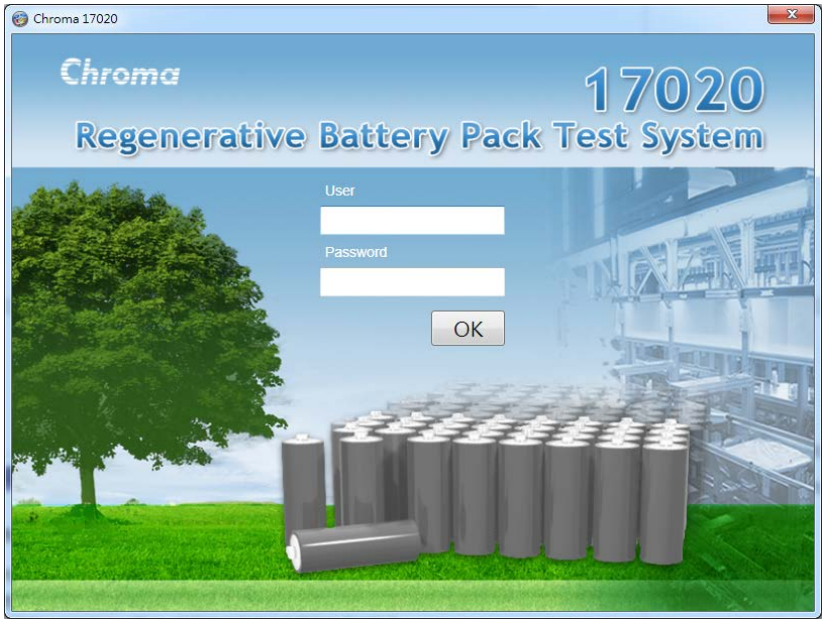
\includegraphics[width=1\linewidth]{Chapters/img/17020_Program/Loggin.png}
		\centering
		\captionsetup{justification=centering,margin=2cm}
		\caption{หน้าเข้าสู่ระบบ}
		\label{fig:Loggin}
	\end{figure}
\end{center}
โดยรหัสผ่านค่าเริ่มต้นจากโรงงานคือ User:root, Password:root เมื่อเข้าสู่ระบบได้แล้วจะพบกับหน้าต่างดังรูปที่\ref{Main_window}
\begin{center}
	\begin{figure}[H]
		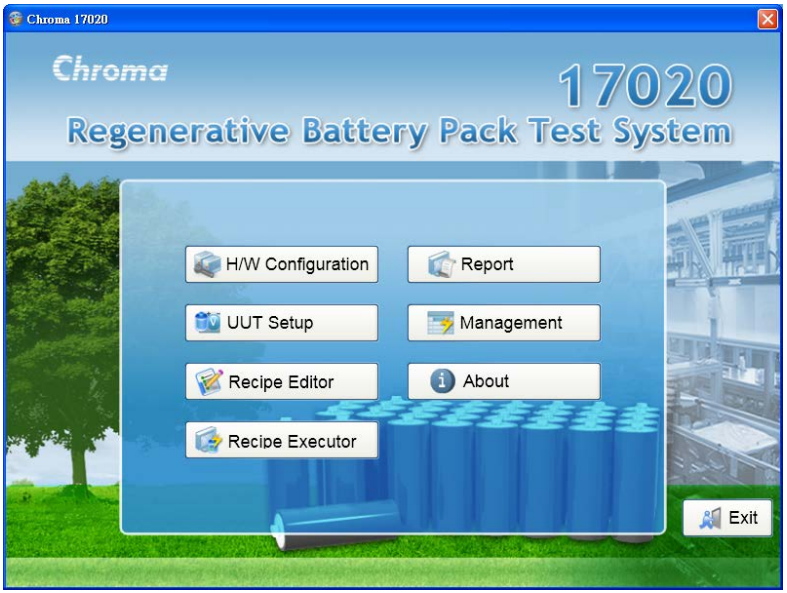
\includegraphics[width=1\linewidth]{Chapters/img/17020_Program/Home.png}
		\centering
		\captionsetup{justification=centering,margin=2cm}
		\caption{หน้าหลัก}
		\label{Main_window}
	\end{figure}
\end{center}
ซึ่งหน้านี้จะหน้าที่ใช้เพื่อเข้าสู่การตั้งค่าและการทำงานต่างๆของเครื่องทดสอบแบตเตอรี่ Chroma 17020 โดยจะประกอบไปด้วย 7 ส่วนดังนี้
\begin{itemize}
{\item H/W Configulation ในส่วนนี้คือส่วนสำหรับการเพิ่มอุปกรณ์วัดและทดสอบและ\\ตั้งค่าอุปกรณ์นั้นๆ}
{\item UUT Setup เป็นส่วนที่ใช้กำหนดขอบเขตของตัวแปรต่างๆ}
{\item Recipe Editor เป็นส่วนที่ตั้งค่าการทดสอบหรือใช้เพื่อกำหนดวิธีการทดสอบ}
{\item Recipe Executor เป็นส่วนที่ทำตามขั้นตอนการทดสอบที่ได้จาก Recipe Editor}
{\item Report เป็นส่วนที่ใช้รายงานผลการทดสอบ}
{\item Management เป็นส่วนที่ใช้สำหรับตั้งค่าอื่นๆในระบบเพิ่มเติม}
{\item About เป็นส่วนที่แสดงข้อมูลเบื้องต้นของระบบเช่น รุ่นของระบบ(Version) ผู้ใช้งาน(User)}
\end{itemize}
%**********************************************************************
\section{การตั้งค่าอุปกรณ์ในระบบ(Hardware Configuration)}
เมื่อเข้าสู่หน้าต่างในส่วนของ H/W Configulation จะพบกับหน้าต่างดังรูป
\begin{center}
	\begin{figure}[H]
		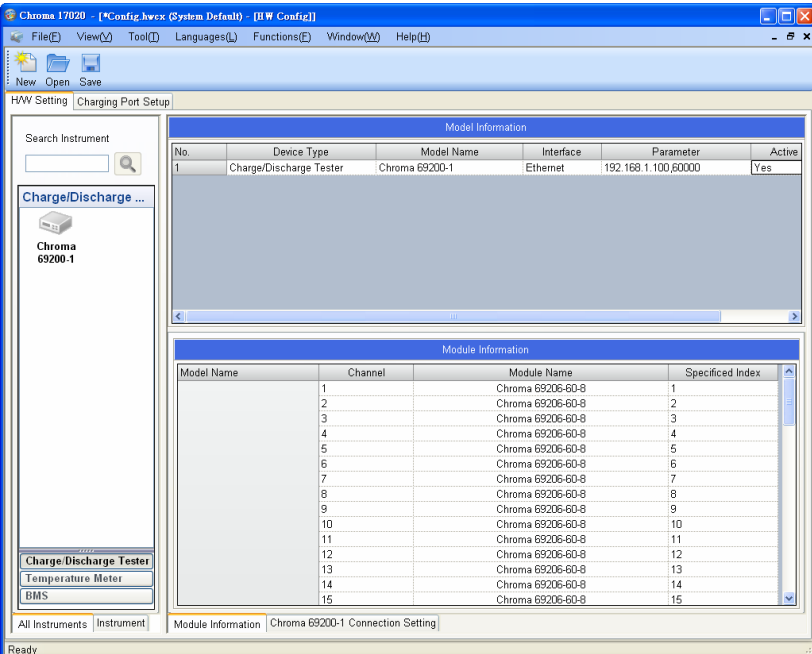
\includegraphics[width=1\linewidth]{Chapters/img/17020_Program/HW_Configulation/Main.png}
		\centering
		\captionsetup{justification=centering,margin=2cm}
		\caption{หน้าต่าง H/W Configulation}
	\end{figure}
\end{center}
โดยหน้าต่างนี้จะประกอบไปด้วย 3 ส่วนคือ
\begin{itemize}
{\item รายการเครื่องมือวัดที่สามารถใช้กับระบบนี้ได้}
{\item รายการเครื่องมือวัดที่เชื่อมต่อและการเชื่อมต่อ}
{\item การเลือกใช้งานเครื่องมือวัดต่อจำนวนอุปกรณ์ที่จะทำการวัด}
\end{itemize}
สำหรับการใช้งานเบื้องต้นถ้าหากต้องการสร้างการตั้งค่าขึ้นใหม่ให้กด file/new ตรงแถบเมนูด้านบนขวาของหน้าต่างนี้จากนั้นให้กด file/Auto Detect เพื่อให้ระบบค้นหาเครื่องมือวัดที่เชื่อมต่ออยู่ในระบบและตั้งค่าเครื่องมือวัดเบื้องต้นให้เองอัตโนมัติซึ่งถ้าหากตั้งค่าแล้วต้องทำการบันทึกข้อมูลทุกครั้งและถ้าหากต้องการใช้การตั้งค่านี้ให้กด file/Set As System Default
ในกรณีที่มีการบันทึกการตั้งค่าแล้วต้องการเรียกดูค่าการตั้งค่านั้นให้กด file/open แล้วเลือกดูการตั้งค่าตามที่ได้ตั้งชื่อไว้
%**********************************************************************
\subsection{ตั้งค่าข้อมูลเครื่องมือวัด(Setting Device Information)}
จากรูปที่ข.4 จะเป็นหน้าต่าง H/W Setting window ในหน้าจะสามารถตั้งค่าข้อมูลเครื่องมือวัดที่เชื่อมต่อเข้าสู่ระบบได้เช่น การเชื่อมต่อ(communication interface)และหมายเลขที่อยู่ไอพีของเครื่องมือวัด(IP Adress)
\newline
%++++++++++++++++++++++++++++++++++++++++++++++++
\newline
\textbf{การเพิ่มเครื่องมือวัดเข้าสู่ระบบ}
\newline \hspace*{2cm} 
การเพิ่มเครื่องมือวัดเข้าสู่ระบบให้จากรูปที่ข.4 คลิ๊กสองครั้งที่รูปเครื่องมือวัดหรือลากลงไปในหน้า All instuments หรือให้เข้าไปที่หน้า Instument คลิ๊กขวาที่จุดรวมเครื่องมือและเลือก Add Device 
ดังรูปที่ข.5 จากนั้นให้คลิ๊กขวาที่รูปเครื่องมือวัดแล้วเลือกเครื่องมือวัดที่ต้องการดังรูปที่ข.6 ซึ่งในตัวอย่างนี้จะเป็นการเลือกเครื่อง Chroma 69200-1 เข้าสู่ระบบจากนั้นเมื่อเลือกเสร็จหน้าต่างดังรูปที่ข.7 จะปรากฎให้กดตกลง
\begin{center}
	\begin{figure}[H]
		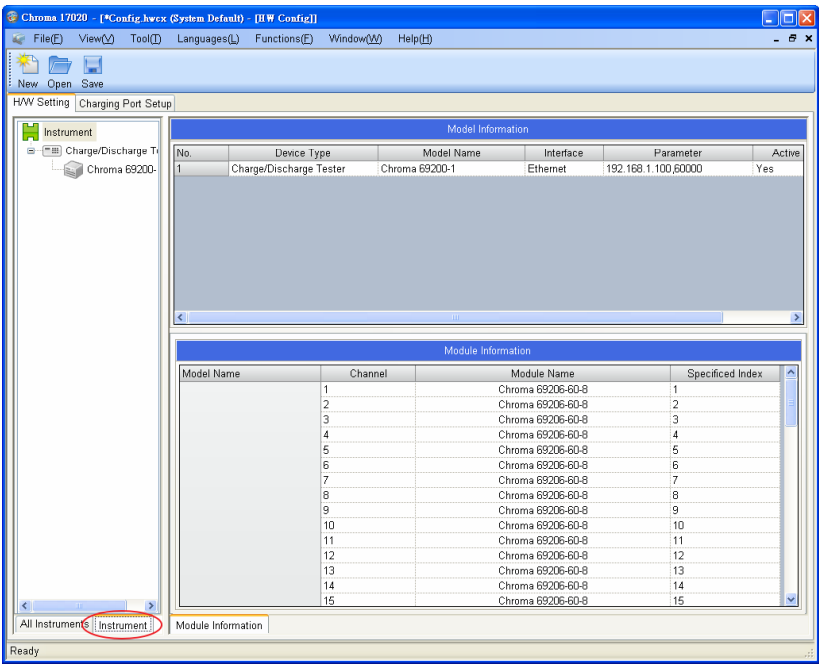
\includegraphics[width=1\linewidth]{Chapters/img/17020_Program/HW_Configulation/Device_Tree.png}
			\centering
			\captionsetup{justification=centering,margin=2cm}
			\caption{หน้า Instument}
	\end{figure}
	\begin{figure}[H]
		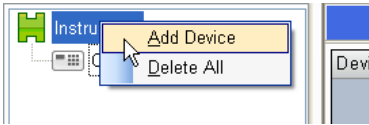
\includegraphics[width=1\linewidth]{Chapters/img/17020_Program/HW_Configulation/Adding_a_device.png}
			\centering
			\captionsetup{justification=centering,margin=2cm}
			\caption{การเพิ่มเครื่องมือวัด}
	\end{figure}
	\begin{figure}[H]
		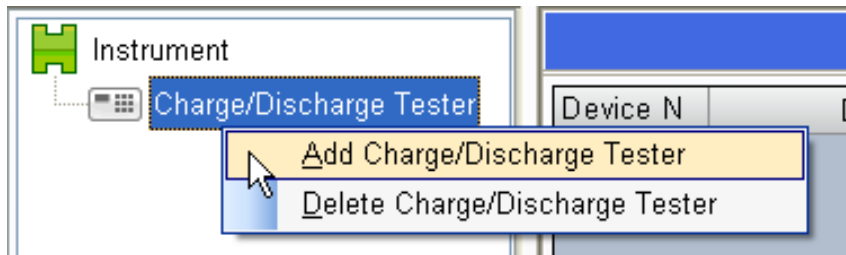
\includegraphics[width=1\linewidth]{Chapters/img/17020_Program/HW_Configulation/Adding_Charge.png}
			\centering
			\captionsetup{justification=centering,margin=2cm}
			\caption{การเพิ่ม Charge/Discharge Tester}
	\end{figure}
	\begin{figure}[H]
		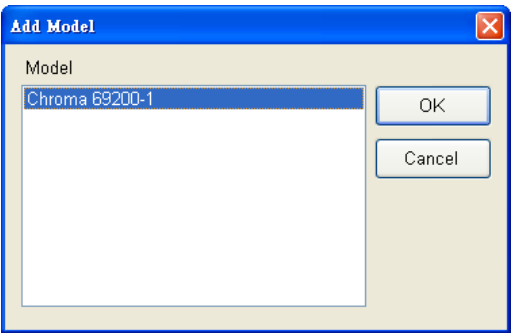
\includegraphics[width=1\linewidth]{Chapters/img/17020_Program/HW_Configulation/Add_Model.png}
			\centering
			\captionsetup{justification=centering,margin=2cm}
			\caption{เลือกรุ่นของเครื่องมือวัด}
	\end{figure}
\end{center}
%++++++++++++++++++++++++++++++++++++++++++++++++
\textbf{การตั้งค่าหมายเลขที่อยู่ไอพี(IP Adress)}
\newline \hspace*{2cm}
ในรูปที่ข.8 จะเป็นตารางข้อมูลการเชื่อมต่อของเครื่องมือวัดต่างๆที่เชื่อมต่ออยู่ในระบบซึ่งถ้าหากต้องการเปลี่ยนแปลงหมายเลยที่อยู่ไอพี(IP Adress)ให้คลิ๊กสองครั้งที่หมายเลขที่อยู่ไอพีที่ต้องการจะตั้งค่า
เมื่อคลิ๊กแล้วจะปรากฎหน้าต่างดังรูปที่ข.9 จากนั้นให้ตั้งค่าตามที่ต้องเมื่อตั้งค่าเสร็จให้กดตกลง
\begin{center}
	\begin{figure}[H]
		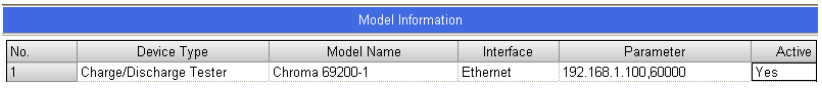
\includegraphics[width=1\linewidth]{Chapters/img/17020_Program/HW_Configulation/Model_info.png}
		\centering
		\captionsetup{justification=centering,margin=2cm}
		\caption{ข้อมูลการเชื่อมต่อของเครื่องมือวัด}
	\end{figure}
	\begin{figure}[H]
		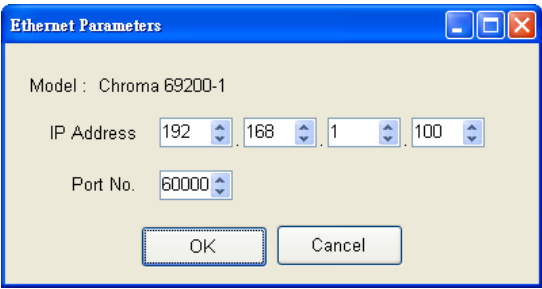
\includegraphics[width=1\linewidth]{Chapters/img/17020_Program/HW_Configulation/IP_Address.png}
		\centering
		\captionsetup{justification=centering,margin=2cm}
		\caption{หน้าต่างการตั้งค่าหมายเลขที่อยู่ไอพี}
	\end{figure}
\end{center}
%++++++++++++++++++++++++++++++++++++++++++++++++
\textbf{ทดสอบการเชื่อมต่อของเครื่องมือวัด(Connection Test)}
\newline \hspace*{2cm}
เมื่อทำการตั้งค่าอุปกรณ์แล้วทำการบันทึกข้อมูลเรียบร้อยแล้วให้ทำการทดสอบการเชื่อมต่อของเครื่องมือวัดโดยให้เข้าไปที่ file/Connection Test แล้วหน้าต่างการทดสอบการเชื่อมต่อจะปรากฎดังรูปที่ข.10
ซึ่งในรูปจะเห็นว่าการทดสอบการเชื่อมต่อของเครื่องมือวัดนั้นเสร็จสิ้นโดยไม่มีข้อผิดพลาด
\begin{center}
	\begin{figure}[H]
		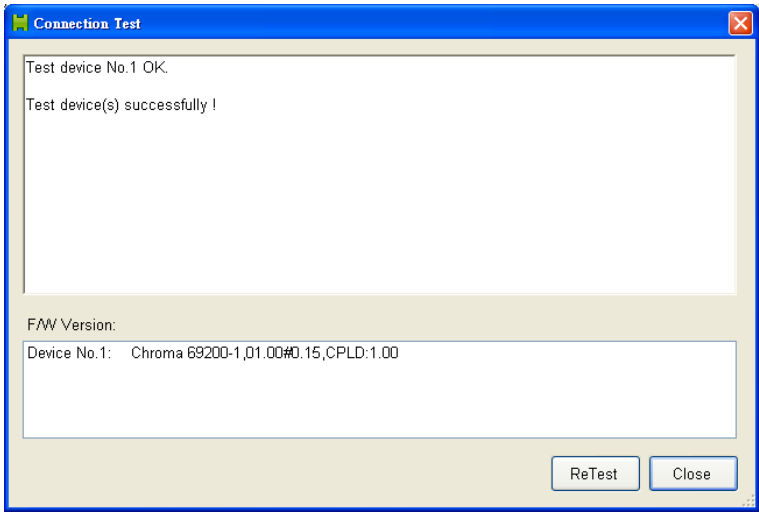
\includegraphics[width=1\linewidth]{Chapters/img/17020_Program/HW_Configulation/Connection_test.png}
		\centering
		\captionsetup{justification=centering,margin=2cm}
		\caption{ข้อมูลการเชื่อมต่อของเครื่องมือวัด}
	\end{figure}
\end{center}
%**********************************************************************
\section{การตั้งค่าขอบเขตตัวแปรต่างๆ(UUT Setup)}
จากหน้าต่างแรกให้คลิ๊กที่ UUT Setup จากนั้นหน้าต่าง UUT Setup จะปรากฎดังรูปที่ข.11 ในหน้านี้เราสามารถตั้งค่าขอบเขตของตัวแปรต่างๆให้เหมาะสมกับการทดสอบแบตเตอรี่ได้เพื่อป้องกันไม่ให้เครื่องอัดและคายประจุ
นั้นอัดประจุหรือคายประจุเกินกว่าที่ได้กำหนดหรือสำหรับอุปกรณ์อื่นก็จะไม่สามารถทำงานเกินกว่าขอบเขตตามที่ได้ตั้งค่าไว้ในหน้าต่างนี้และเมื่อทำการตั้งค่าเสร็จแล้วให้ทำการบันทึกข้อมูล
\begin{center}
	\begin{figure}[H]
		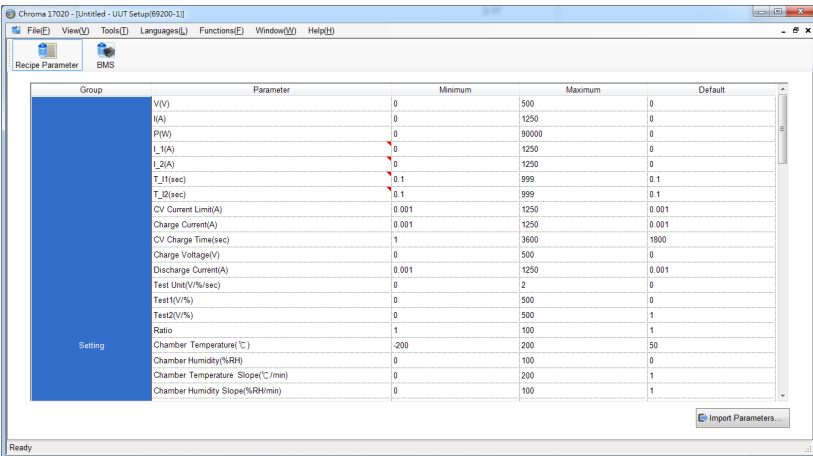
\includegraphics[width=1\linewidth]{Chapters/img/17020_Program/UUT/UUT_setup_win.png}
		\centering
		\captionsetup{justification=centering,margin=2cm}
		\caption{หน้าต่าง UUT Setup}
	\end{figure}
\end{center}
%**********************************************************************
\section{การตั้งค่าการทดสอบหรือวิธีขั้นตอนการทดสอบ(Recipe Editor)}
จากหน้าต่างแรกให้คลิ๊กที่ Recipe Editor จากนั้นหน้าต่าง Recipe Editor จะปรากฎดังรูปที่ข.12 ซึ่งในหน้าต่างนี้จะเป็นหน้าสำคัญที่เอาไว้ใช้กำหนดขั้นตอนการทดสอบและตัวแปรต่างๆสำหรับการทดสอบ
โดยเมื่อได้เข้ามาสู่หน้าต่างนี้ถ้าหากมีข้อมูลที่ได้ทำการบันทึกไว้ก่อนหน้านี้แล้วต้องการจะเรียกข้อมูลให้เลือก Open จากนั้นให้เลือกข้อมูลที่ได้ทำหารบันทึกไว้ก่อนหน้าและกดตกลงดังรูปที่ข.13
ถ้าหาต้องการจะสร้างใหม่ให้เลือก New และกดตกลง
\begin{center}
	\begin{figure}[H]
		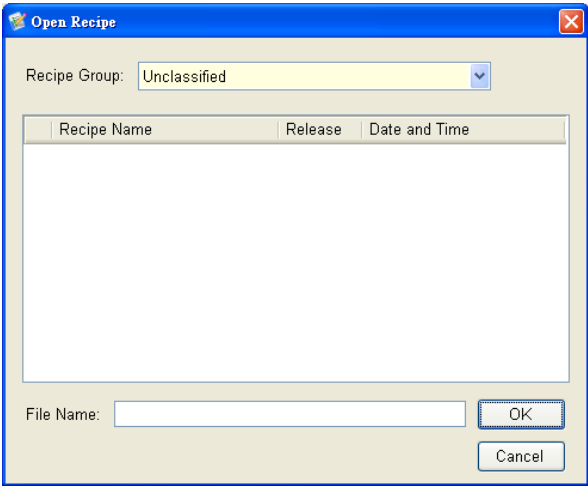
\includegraphics[width=1\linewidth]{Chapters/img/17020_Program/Recipe_Editor/Recipe_dialog.png}
		\centering
		\captionsetup{justification=centering,margin=2cm}
		\caption{หน้าต่างแรกเมื่อเข้าสู่ Recipe Editor}
	\end{figure}
	\begin{figure}[H]
		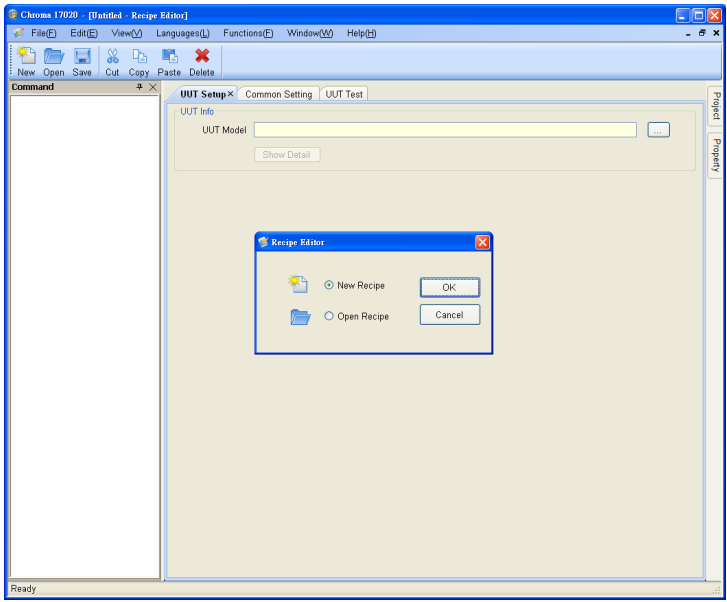
\includegraphics[width=1\linewidth]{Chapters/img/17020_Program/Recipe_Editor/Recipe_editor_win.png}
		\centering
		\captionsetup{justification=centering,margin=2cm}
		\caption{หน้าต่างเลือกข้อมูลการตั้งค่าอื่นๆ}
	\end{figure}
\end{center}
ซึ่งไม่ว่าจะเลือกข้อมูลที่ได้มีการตั้งค่าอยู่แล้วหรือจะสร้างการตั้งค่าใหม่ก็จะเข้าสู่หน้าถัดไปดังรูปข.14 ซึ่งสำหรับการสร้างการตั้งค่าใหม่ให้ทำการเลือกขอบเขตตัวแปรที่ได้จากการตั้งค่าใน UUT Setup ดังกรอบสีแดงดังรูปเมื่อเลือกเสร็จ
ให้กดตกลง และจะเห็นได้ว่าหน้าต่างนี้จะมีแถบหน้าต่างอยู่ทั้งสิ้น 5 ส่วนดังนี้คือ UUT Setup, Common Setting, UUT Test, Protection และ Remote Alarm
\begin{center}
	\begin{figure}[H]
		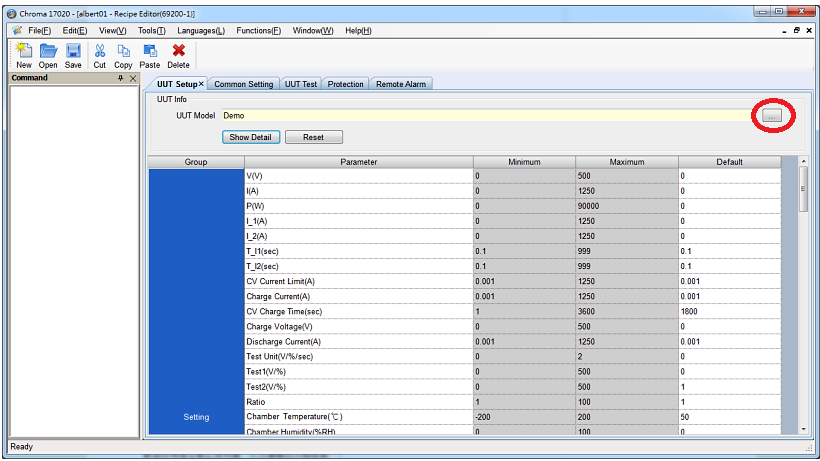
\includegraphics[width=1\linewidth]{Chapters/img/17020_Program/Recipe_Editor/Setting_param_UUT_recipe_editor.png}
		\centering
		\captionsetup{justification=centering,margin=2cm}
		\caption{หน้าต่างแรกเมื่อเข้าสู่ Recipe Editor}
	\end{figure}
\end{center}
%++++++++++++++++++++++++++++++++++++++++++++++++
\textbf{การตั้งค่าการแจ้งเตือน(Remote Alarm)}
\newline \hspace*{2cm}
ในหน้าต่างนี้จะสามารถตั้งค่าการแจ้งเตือนต่างๆได้เมื่อเครื่องมือวัดสมารถตรวจสอบความผิดพลาดหรือค่าตัวแปรต่างๆนั้นเกินขอบเขตที่ได้กำหนดไว้ดังหัวข้อต่างๆถ้าหากต้องการให้มีการแจ้งเตือน
ให้คลิ๊กที่กล่องสี่เหลี่ยมหน้าหัวข้อที่ต้องการให้มีการเเจ้งเตือนดังรูปที่ข.15
\begin{center}
	\begin{figure}[H]
		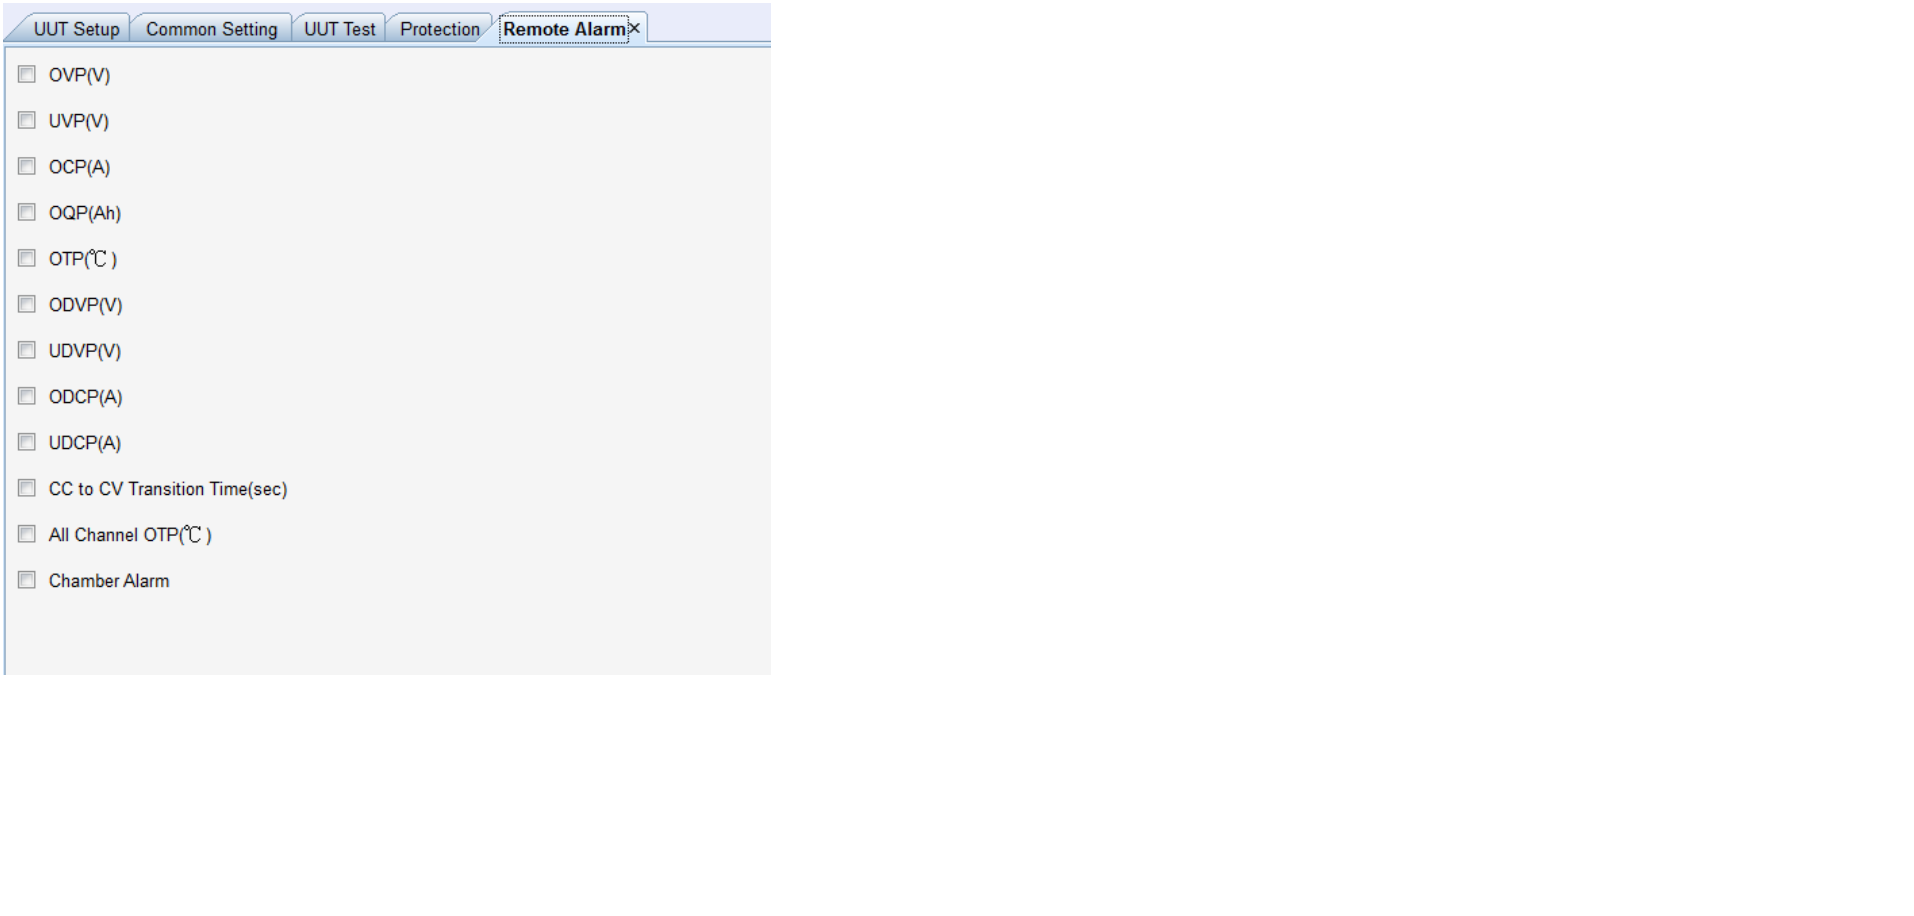
\includegraphics[width=1\linewidth]{Chapters/img/17020_Program/Recipe_Editor/setting_remote_alarm.png}
		\centering
		\captionsetup{justification=centering,margin=2cm}
		\caption{หน้าต่าง Remote Alarm}
	\end{figure}
\end{center}
%++++++++++++++++++++++++++++++++++++++++++++++++
\textbf{การตั้งค่าการป้องกัน(Protection)}
\newline \hspace*{2cm}
ในหน้าต่างนี้จะสามารถตั้งค่าเงื่อนไขการป้องกันในตัวแปรต่างๆได้คล้ายกับการตั้งค่าขอบเขตในหน้าต่าง UUT Setup ซึ่งความแตกต่างระหว่างการตั้งค่าทั้ง 2 นี้คือสำหรับการตั้งค่าขอบเขตนั้นจะเป็นการกำหนดขอบเขตเพื่อไม่ให้
ทำการตั้งค่าอื่นๆในหน้าต่างอื่นๆนั้นจะไม่สามารถตั้งค่าได้เกินขอบเขตที่ได้กำหนดไว้ได้แต่สำหรับการตั้งค่าการป้องกันนั้นจะเป็นการกำหนดเงื่อนไขที่จะทำให้ระบบเครื่องมือวัดของเครื่อง Chroma 17020 นั้นจะทำการหยุดการทดสอบเพื่อ
ป้องกันความเสียหายที่จะเกิดขึ้นกับแบตเตอรี่หรือความเสียหายที่จะเกิดขึ้นกับเครื่องมือวัดได้โดยการตั้งค่าเงื่อนไขในตัวแปรต่างๆจะสามารถตั้งค่าได้ดังรูปที่ข.16
\begin{center}
	\begin{figure}[H]
		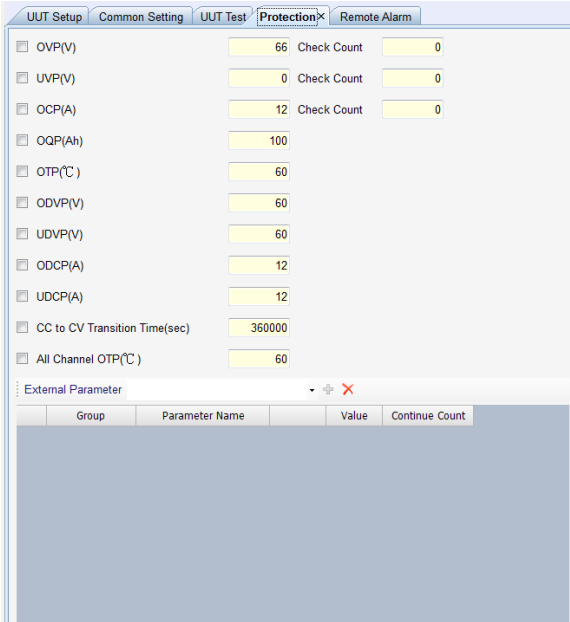
\includegraphics[width=1\linewidth]{Chapters/img/17020_Program/Recipe_Editor/setting_protection.png}
		\centering
		\captionsetup{justification=centering,margin=2cm}
		\caption{หน้าต่าง Protection}
	\end{figure}
\end{center}
%++++++++++++++++++++++++++++++++++++++++++++++++
\textbf{การตั้งค่าขั้นตอนการทดสอบ(UUT Test)}
\newline \hspace*{2cm}
สำหรับหน้าต่างนี้จะเป็นหน้าต่างที่มีความสำคัญลำดับต้นๆเนื่องจากหน้าต่างนี้จะใช้สำหรับในการตั้งค่าการกำหนดขั้นตอนการทดสอบแบตเตอรี่ของระบบเช่น การอัดประจุ การคายประจุ เป็นต้นโดยหน้าต่างนี้จะมีลักษณะดังรูปที่ข.17
ซึ่งจะประกอบไปด้วย 3 ส่วนหลักคือ 
\begin{itemize}
{\item คำสั่งต่างๆที่ใช้สำหรับการทดสอบ}
{\item ลำดับขั้นตอนของคำสั่งในการทดสอบ}
{\item การตั้งค่าเพิ่มเติม}
\end{itemize}
\begin{center}
	\begin{figure}[H]
		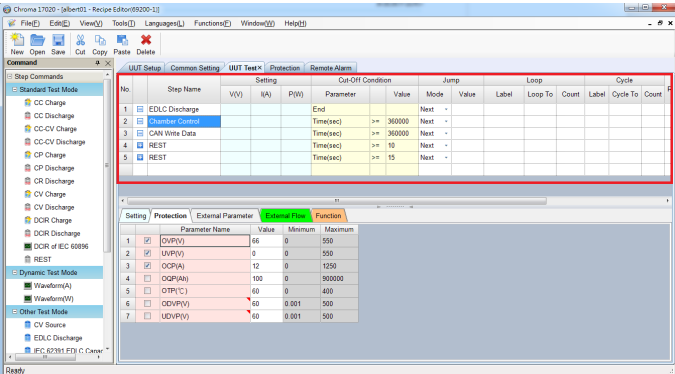
\includegraphics[width=1\linewidth]{Chapters/img/17020_Program/Recipe_Editor/UUT_tesing_page.png}
		\centering
		\captionsetup{justification=centering,margin=2cm}
		\caption{หน้าต่าง Protection}
	\end{figure}
\end{center}
โดยในส่วนลำดับขั้นตอนของคำสั่งซึ่งคำสั่งต่างๆจะถูกจัดลำดับการทำงานเป็นตารางซึ่งในการเพิ่มคำสั่งให้คลิ๊กที่ตารางแล้วจากนั้นให้คลิ๊ก 2 ครั้งที่คำสั่งที่ต้องการจะเพิ่มแล้วคำสั่งจะถูกเพิ่มเข้ามาอยู่ในตารางในกรณีที่ต้องการเพิ่มคำสั่งที่
เหมือนกับคำสั่งก่อนหน้าให้คลิ๊กที่คำสั่งที่ต้องการคัดลอกแล้วกดคัดลอก(Copy)ตรงแถบด้านบนดังรูปที่ข.17 จากนั้นให้กดวาง(Past)ที่ตารางลำดับคำสั่งแล้วคำสั่งที่ได้ทำการคัดลอกจะมาปรากฎอยู่ในตารางซึ่งตัวแปรต่างๆ
ที่ได้ทำการตั้งค่าไว้แล้วก่อนหน้าเมื่อกดวางแล้วคำสั่งใหม่ที่ถูกเพิ่มเข้ามานั้นจะมีการตั้งค่าที่เหมือนกันทุกประการหากต้องการที่จะลบคำสั่งให้คลิ๊กที่คำสั่งหนึ่งครั้งแล้วกดลบ(Delete) 
\newline \hspace*{2cm}
สำหรับส่วนประกอบต่างๆในตารางลำดับคำสั่งโดยเรียงลำดับจากซ้ายไปขวาจะมีดังนี้
\begin{itemize}
{\item (No.) ลำดับคำสั่ง}
{\item (Step Name) ชื่อคำสั่ง}
{\item (Setting) ค่าตัวแปรสำหรับคำสั่งคือ แรงดันไฟฟ้าV(V) กระแสไฟฟ้าI(A) กำลังไฟฟ้าP(W) โดยในส่วนนี้สามารถกำหนดค่าได้}
{\item (Cut-Off Condition) เงื่อนไขการสิ้นสุดคำสั่งนั้นๆ}
{\item (Jump) ขั้นตอนการทำงานถัดไปเมื่อสิ้นสุดคำสั่งนั้นๆโดยสามารถเลือกได้ดังนี้คือ ทำคำสั่งถัดไปในตาราง(Next),\newline สิ้นสุดการทำงาน(End), 
ข้ามไปทำคำสั่งที่ได้ตั้งค่าไว้(Jump to Step),พักชั่วคราวตามที่ได้ตั้งค่าไว้ในหน่วยวินาที(Rest),ทำตามเงื่อนไข(If)และ}
{\item (Loop) กำหนดการทำคำสั่งซ้ำ (Label)เป็นคอลัมน์ที่ใช้เพื่อกำหนดคำสั่งที่ต้องการทำซ้ำ (Loop to)เป็นคอลัมน์ที่ใช้เพื่อกำหนดคำสั่งที่ต้องการทำซ้ำไปถึงคำสั่งที่มีการกำหนด\newline
	    (Count) กำหนดจำนวนครั้งที่ต้องการทำซ้ำ}
\end{itemize}
%************************************************************************************************************
\section{การสั่งการทำงานตามขั้นตอนการทดสอบ(Recipe Executor)}
คลิ๊กที่เมนู Recipe Executor จากหน้าต่างหลักเพื่อเข้าสู่หน้าต่างการทำงานนี้ดังในรูป\ref{fig:main_Recipe_Executor}ซึ่งในรูปจะแสดงช่องทางการทดสอบแบตเตอรี่ที่สามารถใช้ในการทดสอบได้
ทั้งหมด
\begin{center}
	\begin{figure}[H]
		\includegraphics[width=1\linewidth]{Chapters/img/17020_Program/Recipe_Executor/Recipe_executor_main_win.png}
		\centering
		\captionsetup{justification=centering,margin=2cm}
		\caption{หน้าต่างหลัก Recipe Executor}
		\label{fig:main_Recipe_Executor}
	\end{figure}
\end{center}
ในการเลือกช่องทางในการทดสอบแบตเตอรี่ที่ต้องการสามารถกดเลือกช่องสี่เหลี่ยมตรงช่องทางที่ต้องการดังรูปที่\ref{fig:select_box} จากนั้นให้ทำการเลือกขั้นตอนการทดสอบที่ได้ทำการตั้งค่าไว้แล้วดังรูปที่\ref{fig:data_display_recipe_executor} ในกรณีที่ไม่มีรูป(Icon)แสดงขึ้นมาดังในวงกลมสีแดงให้ทำการกดที่คำว่า Recipe Name แทนเมื่อคลิ๊กเข้าไปแล้วจะพบกับหน้าต่างดังรูปที่\ref{fig:recipe_setup_win}ให้ทำการเลือกชื่อลำดับขั้นตอนที่ได้ตั้งค่าไว้แล้วจากเมนู Recipe Editor โดยเลือกขั้นตอนที่ต้องการ
ให้ตรงกับช่องทางการทดสอบที่ต้องการจากนั้นให้กดตกลงจากนั้นให้กด Start จากเมนูด้านบนในรูปที่\ref{fig:main_Recipe_Executor}หลังจากที่ได้เริ่มทำการทดสอบแล้วโดยถ้าหากต้องการดูข้อมูลการทดสอบ
ให้กดที่รูปกล่องสีเขียวจากนั้นกราฟข้อมูลการทดสอบจะปรากฎขึ้นดังรูปที่\ref{fig:ch_graph}

\begin{center}
	\begin{figure}[H]
		\centering
		\includegraphics[width=1\linewidth]{Chapters/img/17020_Program/Recipe_Executor/battery_select_box.png}
		\centering
		\captionsetup{justification=centering,margin=2cm}
		\caption{เลือกช่องทางการทดสอบ}
		\label{fig:select_box}
	\end{figure}
	\begin{figure}[H]
		\includegraphics[width=1\linewidth]{Chapters/img/17020_Program/Recipe_Executor/battery_data_display.png}
		\centering
		\captionsetup{justification=centering,margin=2cm}
		\caption{เลือกขั้นตอนการทดสอบ (ก.)}
		\label{fig:data_display_recipe_executor}
	\end{figure}
	\begin{figure}[H]
		\includegraphics[width=1\linewidth]{Chapters/img/17020_Program/Recipe_Executor/recipe_setup_win.png}
		\centering
		\captionsetup{justification=centering,margin=2cm}
		\caption{เลือกขั้นตอนการทดสอบ (ข.)}
		\label{fig:recipe_setup_win}
	\end{figure}
	\begin{figure}[H]
		\includegraphics[width=1\linewidth]{Chapters/img/17020_Program/Recipe_Executor/ch_graph.png}
		\centering
		\captionsetup{justification=centering,margin=2cm}
		\caption{กราฟข้อมูลระหว่างการทดสอบ}
		\label{fig:ch_graph}
	\end{figure}
\end{center}
%************************************************************************************************************
\section{การแสดงผลข้อมูลที่ได้จากการทดสอบ(Report)}
กดเข้าเมนู Report จากในหน้าต่างหลักเพื่อเข้าสู่เมนูนี้แล้วหน้าต่างเมนู Report จะปรากฎดังรูปที่\ref{fig:report}จากนั้นให้เลือกข้อมูลที่ต้องการแสดงผลโดยกดเลือกที่ Generate เมื่อกดเข้าไปแล้ว
หน้าต่างเลือกข้อมูลจะปรากฏดังรูปที่\ref{fig:Selecting_data_data_analysis} จากนั้นให้ทำการเลือกข้อมูลเมื่อเลือกข้อมูลที่ต้องการแล้วให้กดตกลงจากนั้นให้กด Export to PDF
ตรงแถบเมนูด้านบนซึ่งข้อมูลที่ได้นี้จะเป็นข้อมูลอย่างคร่าวๆ
\begin{center}
	\begin{figure}[H]
		\includegraphics[width=1\linewidth]{Chapters/img/17020_Program/Report/Report_main_menu.png}
		\centering
		\captionsetup{justification=centering,margin=2cm}
		\caption{หน้าต่างหลักของเมนู Report}
		\label{fig:report}
	\end{figure}
	\begin{figure}[H]
		\includegraphics[width=1\linewidth]{Chapters/img/17020_Program/Report/Selecting_data.png}
		\centering
		\captionsetup{justification=centering,margin=2cm}
		\caption{หน้าต่างหลักของเมนู Report}
		\label{fig:Selecting_data_data_analysis}
	\end{figure}
\end{center}
โดยการนำข้อมูลการทดสอบอย่างละเอียดให้กดที่เมนู Data Analysis ที่แถบเมนูด้านบนแล้วหน้าต่างจะปรากฎขึ้นดังรูปที่\ref{fig:Data_analysis}โดยในหน้าต่างนี้จะเห็นได้ว่าด้านล่างของหน้าต่าง
จะมีให้กำหนดตัวแปรและแกนที่ต้องการจะวาดกราฟข้อมูลการทดสอบเมื่อกำหนดตัวแปรตามที่ต้องการแล้วให้กดเลือกข้อมูลที่ต้องการที่แถบเมนู Data Selection โดยต้องเลือกให้ตรงกับตัวแปรและแกนที่ได้กำหนดไว้แล้ว
จากนั้นเมื่อเลือกข้อมูลที่ต้องการได้แล้วให้ทำการกด Preview โปรแกรมจะทำการวาดกราฟข้อมูลการทดสอบตามข้อมูลที่ได้เลือกไว้จากนั้นให้กดเลือกเมนู Data เพื่อตรวจสอบความถูกต้องของข้อมูลการทดสอบโดยข้อมูลจะถูกแสดงผล
ออกมาในรูปแบบตารางดังรูปที่\ref{fig:Data_analysis_preview}เมื่อตรวจสอบความถูกต้องของข้อมูลการทดสอบที่ต้องการจะนำไปวิเคราะห์แล้วให้ทำการกดบันทึกข้อมูลโดยเลือกที่เมนู Data Analysis
Export จากนั้นหน้าต่างบันทึกข้อมูลจะปรากฎดังรูปที่\ref{fig:Export_data_analysis} จากนั้นให้ทำการตั้งชื่อและเลือกที่อยู่ของข้อมูลที่ต้องการบันทึกจากนั้นให้กดตกลง

\begin{center}
	\begin{figure}[H]
		\includegraphics[width=1\linewidth]{Chapters/img/17020_Program/Report/Data_analysis.png}
		\centering
		\captionsetup{justification=centering,margin=2cm}
		\caption{หน้าต่างเมนู Data Analysis}
		\label{fig:Data_analysis}
	\end{figure}
	\begin{figure}[H]
		\includegraphics[width=1\linewidth]{Chapters/img/17020_Program/Report/Data_analysis_preview.png}
		\centering
		\captionsetup{justification=centering,margin=2cm}
		\caption{กราฟข้อมูลการทดสอบโดยเมนู Data Analysis}
		\label{fig:Data_analysis_preview}
	\end{figure}
	\begin{figure}[H]
		\includegraphics[width=1\linewidth]{Chapters/img/17020_Program/Report/Export_data_analysis.png}
		\centering
		\captionsetup{justification=centering,margin=2cm}
		\caption{หน้าต่างบันทึกข้อมูลจากเมนู Data Analysis}
		\label{fig:Export_data_analysis}
	\end{figure}
\end{center}

































































































































































































































































































%	%\makeatletter
%\oldchapter*{ประวัติผู้เขียน}
%\addcontentsline{toc}{chapter}{ประวัติผู้เขียน}
%\begin{longtable}{@{}p{0.34\linewidth}@{}p{0.66\linewidth}@{}}
%	ชื่อ									& \@nametitle\@authorThai\\
%	วันเดือนปีเกิด							& \@dateofbirth\\
%	วุฒิการศึกษา			 & \parbox[t]{\linewidth}{\strut\@eduattainment\strut}\\
%	\ifdefined\@workposition ตำแหน่ง	& \@workposition\\\fi
%	\ifdefined\@scholarship ทุนการศึกษา		& \parbox[t]{\linewidth}{\strut\@scholarship\strut}\\\fi
%\end{longtable}
%\noindent ผลงานทางวิชาการ\vspace{\baselineskip}\newline
%\includecollection{publications}\vspace{0.5\baselineskip}
%\ifdefined\@workposition
%\begin{longtable}{@{}p{0.34\linewidth}@{}p{0.66\linewidth}@{}}
%	ประสบการณ์ทำงาน					& \parbox[t]{\linewidth}{\strut\@workexperiences\strut}\\
%\end{longtable}
%\fi
%\makeatother
\oldchapter*{ประวัติผู้เขียน}
\addcontentsline{toc}{chapter}{ประวัติผู้เขียน}
\begin{center}
\begin{longtable}{@{}p{0.34\linewidth}@{}p{0.66\linewidth}@{}}
\includegraphics[scale=0.2,valign=c]{Chapters/img/nisit img/6230304287.jpg} & \\
    &\\
	ชื่อ							& นายณัฐนนท์ กาญจนประภาส\\
	วันเดือนปีเกิด						& วันจันทร์ที่ 14 สิงหาคม พ.ศ.2543\\
	คณะ							& วิศวกรรมศาสตร์ศรีราชา\\
	ภาควิชา							& วิศวกรรมไฟฟ้าและอิเล็กทรอนิกส์\\
	สถาบันการศึกษา						& มหาวิทยาลัยเกษตรศาสตร์วิทยาเขตศรีราชา\\
	รหัสนิสิต						& 6230304287\\
	ที่อยู่ปัจจุบัน						& 272/131 ม.5 ต.นาเกลือ อ.บางละมุง จ.ชลบุรี 20150\\
	โทรศัพท์เคลื่อนที่					& 0874295466\\
	E-mail						& Nuntanon.k@ku.th\\
\end{longtable}

\begin{longtable}{@{}p{0.3\linewidth}@{}p{0.45\linewidth}@{}p{0.25\linewidth}}
	\textbf{ประวัติการศึกษา} & &\\
	คุณวุฒิการศึกษา		&	สถาบัน				&	ปีการศึกษาที่จบ \\\hline
	มัธยมศึกษาตอนต้น	&	โรงเรียนโพธิสัมพันธ์พิทยาคาร	&	2559 	\\
	มัธยมศึกษาตอนปลาย	&	โรงเรียนโพธิสัมพันธ์พิทยาคาร	&	2562 	\\
\end{longtable}
\end{center}
\pagebreak
\oldchapter*{ประวัติผู้เขียน}
\begin{center}
\begin{longtable}{@{}p{0.34\linewidth}@{}p{0.66\linewidth}@{}}
\includegraphics[scale=0.2,valign=c]{Chapters/img/nisit img/6230304287.jpg} & \\
    &\\
	ชื่อ							& นายณัฐนันท์ อุบลวัจ\\
	วันเดือนปีเกิด						& วันจันทร์ที่ 24 กรกฎาคม พ.ศ.2543\\
	คณะ							& วิศวกรรมศาสตร์ศรีราชา\\
	ภาควิชา							& วิศวกรรมไฟฟ้าและอิเล็กทรอนิกส์\\
	สถาบันการศึกษา						& มหาวิทยาลัยเกษตรศาสตร์วิทยาเขตศรีราชา\\
	รหัสนิสิต						& 6230304295\\
	ที่อยู่ปัจจุบัน						& 197 ม.12 ต.หัวไผ่ อ.เมือง จ.สิงห์บุรี 16000\\
	โทรศัพท์เคลื่อนที่					& 0931470597\\
	E-mail						& Natthanan.o@ku.th\\
\end{longtable}

\begin{longtable}{@{}p{0.4\linewidth}@{}p{0.35\linewidth}@{}p{0.25\linewidth}}
	\textbf{ประวัติการศึกษา} & &\\
	คุณวุฒิการศึกษา		&	สถาบัน				&	ปีการศึกษาที่จบ \\\hline
	มัธยมศึกษาตอนต้น	&	โรงเรียนสิงห์บุรี	&	2558 	\\
	มัธยมศึกษาตอนปลาย	&	โรงเรียนสิงห์บุรี	&	2561 	\\
\end{longtable}
\end{center}
\end{document}